\chapter{Representative numerical simulations -- II}
\label{numerical-simulations-2}

\todo{\begin{itemize}
  \item Work on this after, and in tandem with, Chapter 4
  \item Weave around the monolithic implementation details and refer
    COMSOL's documentation to see how it goes about doing things?
    (Cite back to the fact that monolithic is stable.)
  \item Figure out the feasibility of: elastica, visco-poro-elasticity
    friction-coeff. variation or drop the entire section.
  \item Generate pristine plots for the flow field calculations and
    write up elaborate descriptions of the problems, citing back to
    the boundary conditions/saturation constraint of the previous
    chapter. Justify 2D.
  \item Bring in a few experimental figures and point out what we're
    looking for in terms of biphasic response.
  \item Go through cool/realistic calculations and replot a few from
    useful cases. Look at the new proposal to see what is sellable.
  \item Cite work from cancer to motivate the example. Generate many
    plots of the different fields and describe in great detail the toy
    problem citing back to Onsager reciprocity.
\end{itemize}}

\section{The coupled solution scheme}
\label{coupled-solution-scheme-2}

The second set of numerical simulations reside here.

\section{Simple physical tests}
\label{simple-physics}

\subsection{The swelling balloon}
\label{balloon}

\begin{figure}[!hptb]
\centering
\includegraphics[width=0.8\textwidth]{images/examples/%
eulerian/swelling/balloon-swell-0p0}
\caption{The swelling balloon at time $t=0$ s.} 
\label{swelling-balloon-image-0p0}
\end{figure}

\begin{figure}[!hptb]
\centering
\includegraphics[width=0.8\textwidth]{images/examples/%
eulerian/swelling/balloon-swell-0p6}
\caption{The swelling balloon at time $t=0.6$ s.} 
\label{swelling-balloon-image-0p6}
\end{figure}

\begin{figure}[!hptb]
\centering
\includegraphics[width=0.8\textwidth]{images/examples/%
eulerian/swelling/balloon-swell-1p2}
\caption{The swelling balloon at time $t=1.2$ s.} 
\label{swelling-balloon-image-1p2}
\end{figure}

\begin{figure}[!hptb]
\centering
\includegraphics[width=0.8\textwidth]{images/examples/%
eulerian/swelling/balloon-swell-1p8}
\caption{The swelling balloon at time $t=1.8$ s.} 
\label{swelling-balloon-image-1p8}
\end{figure}

\begin{figure}[!hptb]
\centering
\includegraphics[width=0.8\textwidth]{images/examples/%
eulerian/swelling/balloon-swell-2p4}
\caption{The swelling balloon at time $t=2.4$ s.} 
\label{swelling-balloon-image-2p4}
\end{figure}

\begin{figure}[!hptb]
\centering
\includegraphics[width=0.8\textwidth]{images/examples/%
eulerian/swelling/balloon-swell-3p0}
\caption{The swelling balloon at time $t=3.0$ s.} 
\label{swelling-balloon-image-3p0}
\end{figure}

\subsection{The tissue under constriction}
\label{constriction-2}

\begin{figure}[!hptb]
\centering
\includegraphics[width=0.8\textwidth]{images/examples/%
eulerian/constriction/constrict-0p0}
\caption{The constricted tissue at time $t=0$ s.} 
\label{constrict-image-0p0}
\end{figure}

\begin{figure}[!hptb]
\centering
\includegraphics[width=0.8\textwidth]{images/examples/%
eulerian/constriction/constrict-0p32}
\caption{The constricted tissue at time $t=0.32$ s.} 
\label{constrict-image-0p32}
\end{figure}

\begin{figure}[!hptb]
\centering
\includegraphics[width=0.8\textwidth]{images/examples/%
eulerian/constriction/constrict-0p66}
\caption{The constricted tissue at time $t=0.66$ s.} 
\label{constrict-image-0p66}
\end{figure}

\begin{figure}[!hptb]
\centering
\includegraphics[width=0.8\textwidth]{images/examples/%
eulerian/constriction/constrict-1p0}
\caption{The constricted tissue at time $t=1.0$ s.} 
\label{constrict-image-1p0}
\end{figure}

\begin{figure}[!hptb]
\centering
\includegraphics[width=0.8\textwidth]{images/examples/%
eulerian/constriction/constrict-2p0}
\caption{The constricted tissue at time $t=2.0$ s.} 
\label{constrict-image-2p0}
\end{figure}

\begin{figure}[!hptb]
\centering
\includegraphics[width=0.8\textwidth]{images/examples/%
eulerian/constriction/constrict-3p0}
\caption{The constricted tissue at time $t=3.0$ s.} 
\label{constrict-image-3p0}
\end{figure}

\begin{figure}[!hptb]
\centering
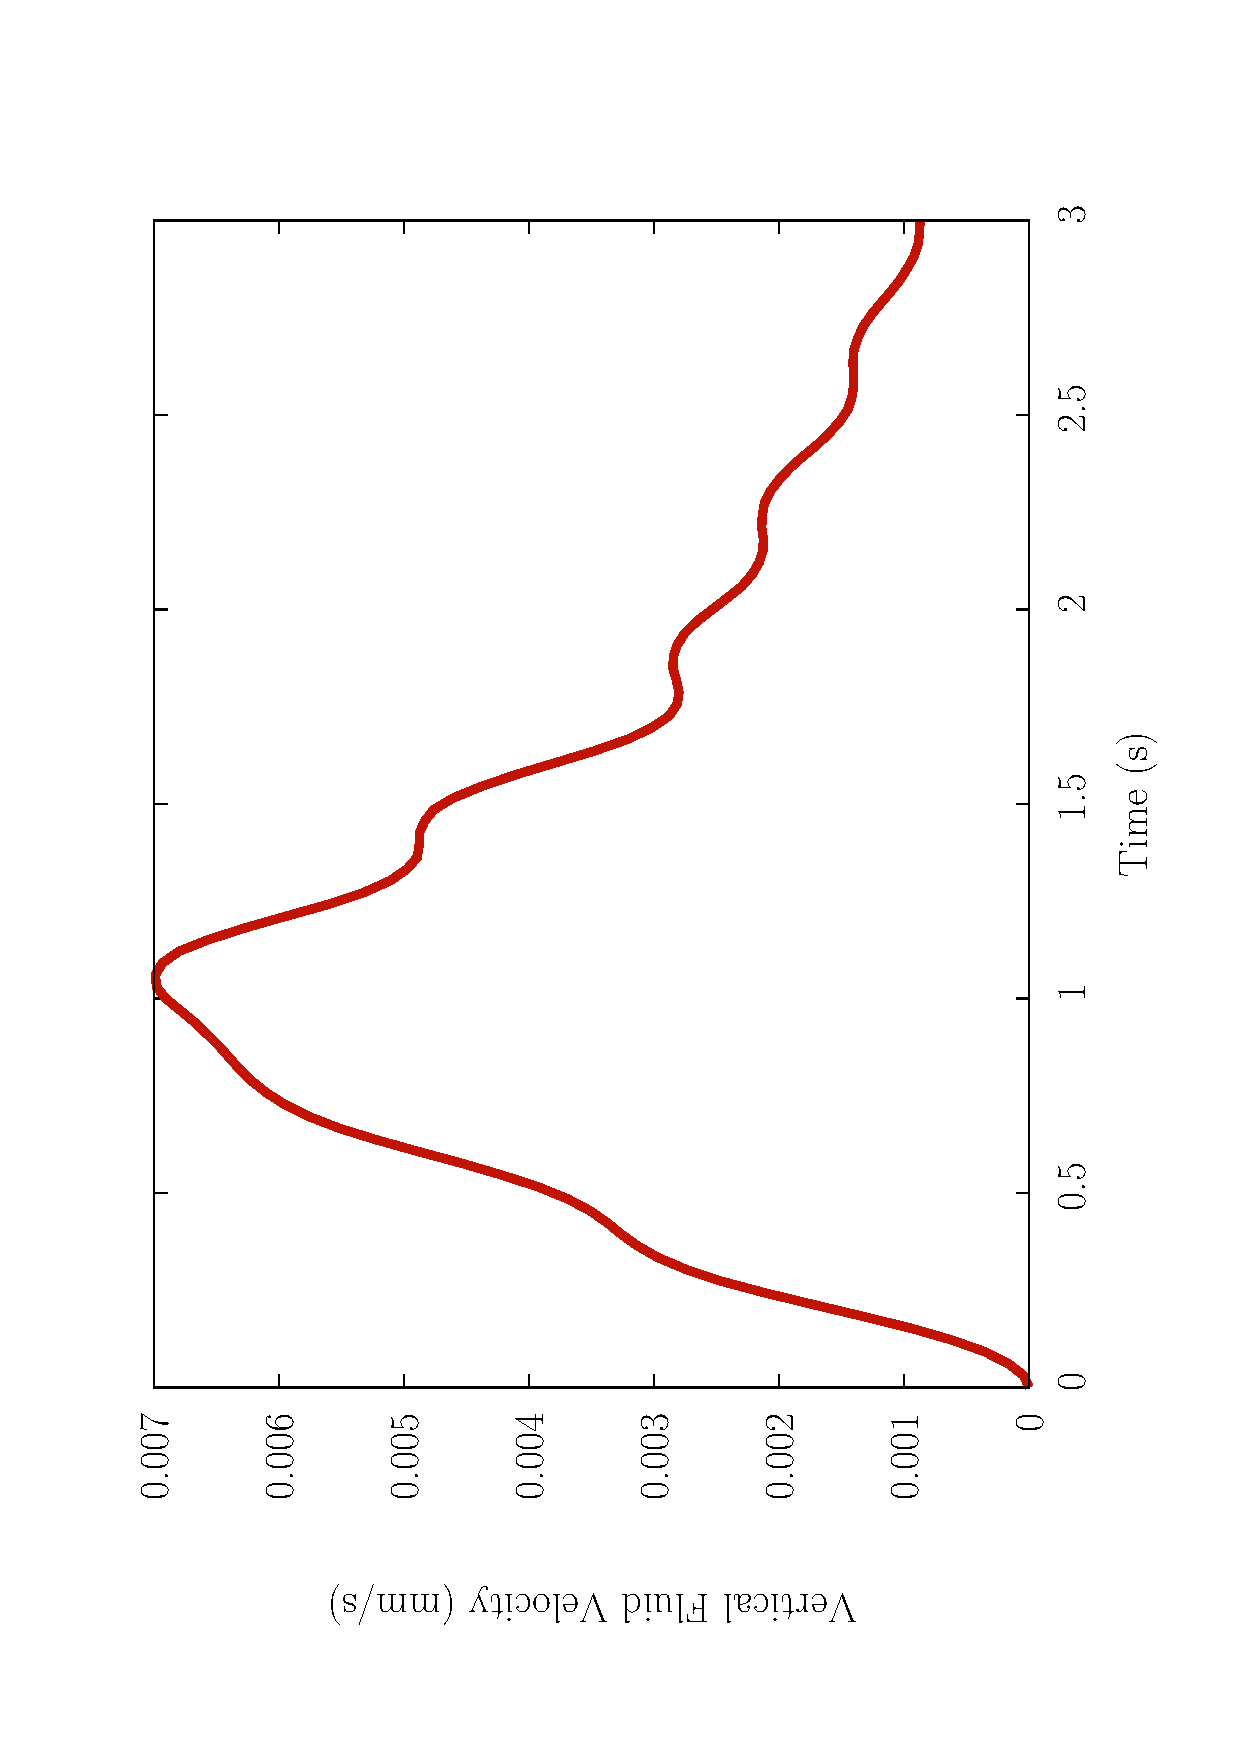
\includegraphics[width=0.6\textwidth,angle=270]{images/examples/%
eulerian/constriction/constrict-vel-drop-dynamic}
\caption{Vertical fluid velocity evolution with dynamics.} 
\label{velocity-evolution-dynamic}
\end{figure}

\begin{figure}[!hptb]
\centering
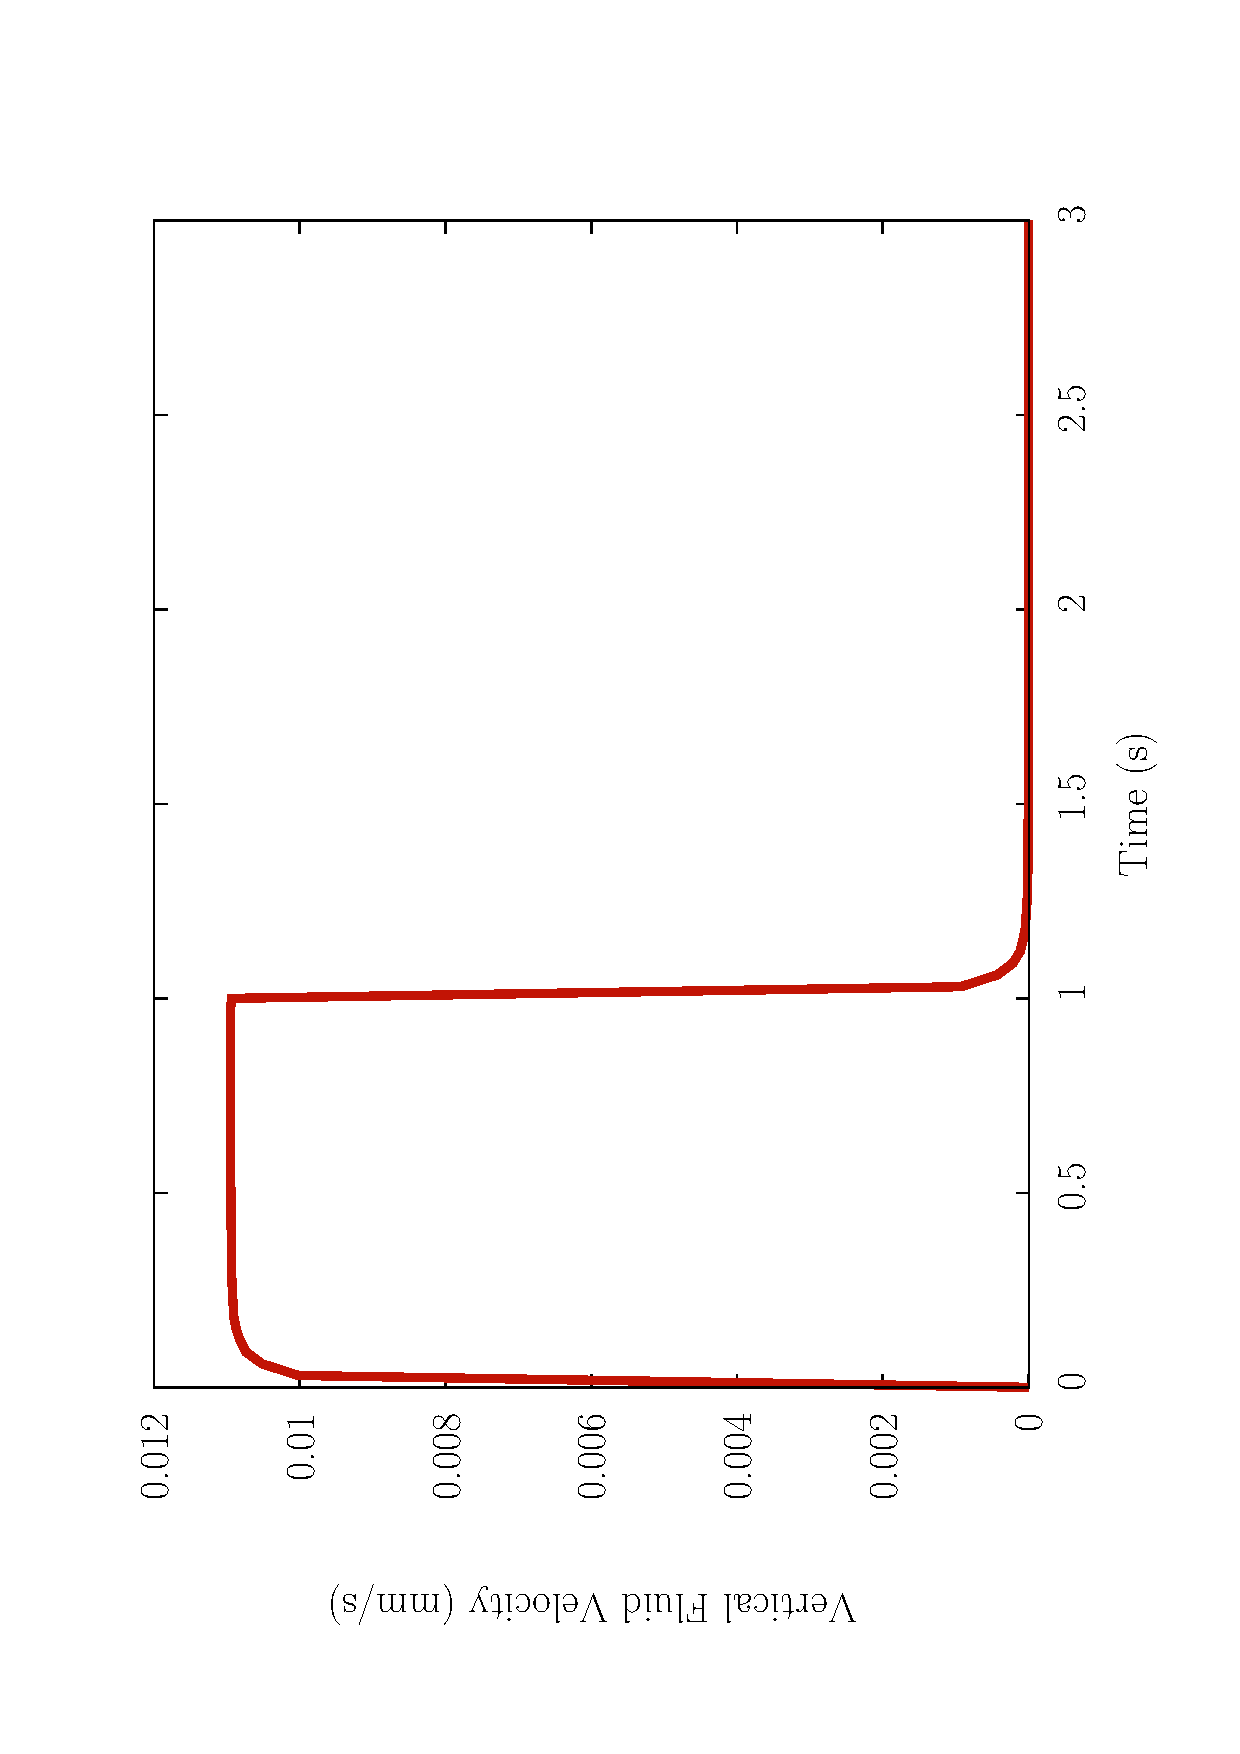
\includegraphics[width=0.6\textwidth,angle=270]{images/examples/%
eulerian/constriction/constrict-vel-drop-quasistatic}
\caption{Vertical fluid velocity evolution with quasistatics.} 
\label{velocity-evolution-quasistatic}
\end{figure}

\subsection{Flow fields under tension}
\label{tension-flow}

\section{Examples exploring the biphasic nature of porous soft tissue}
\label{biphasic-examples-2}

\subsection{Stress relaxation}
\label{stress-relaxation}

\subsubsection{Under different rates of loading}
\label{modifying-load-rates}

\begin{figure}[!hptb]
\centering
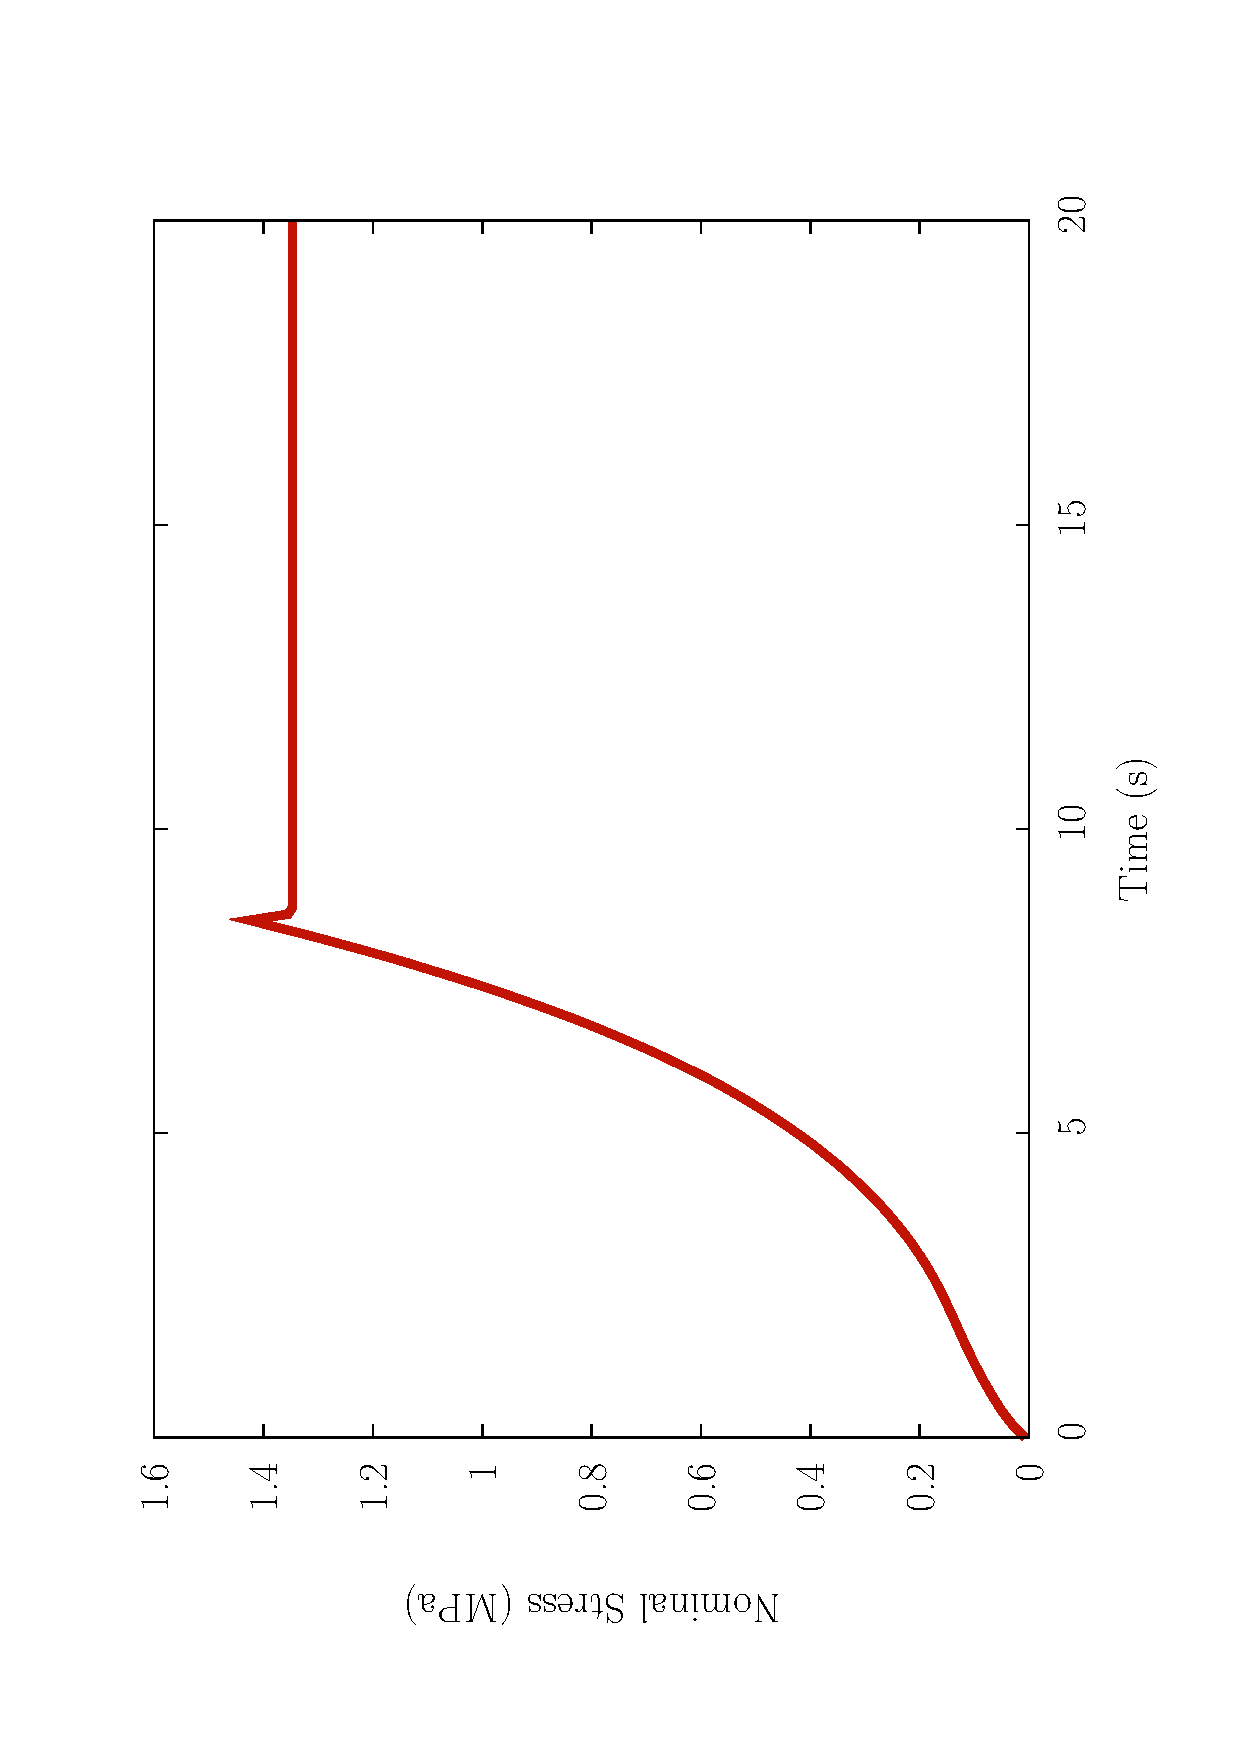
\includegraphics[width=0.6\textwidth,angle=270]{images/examples/%
eulerian/pulling/plots/poro-elastic/poro-stress-relax-0p01}
\caption{Dynamic poroelastic model, $\dot{\epsilon}=0.01$ Hz, $D=1.037$
  MPa.s.mm$^{-1}$.}
\label{poro-stress-relax-0p01}
\end{figure}

\begin{figure}[!hptb]
\centering
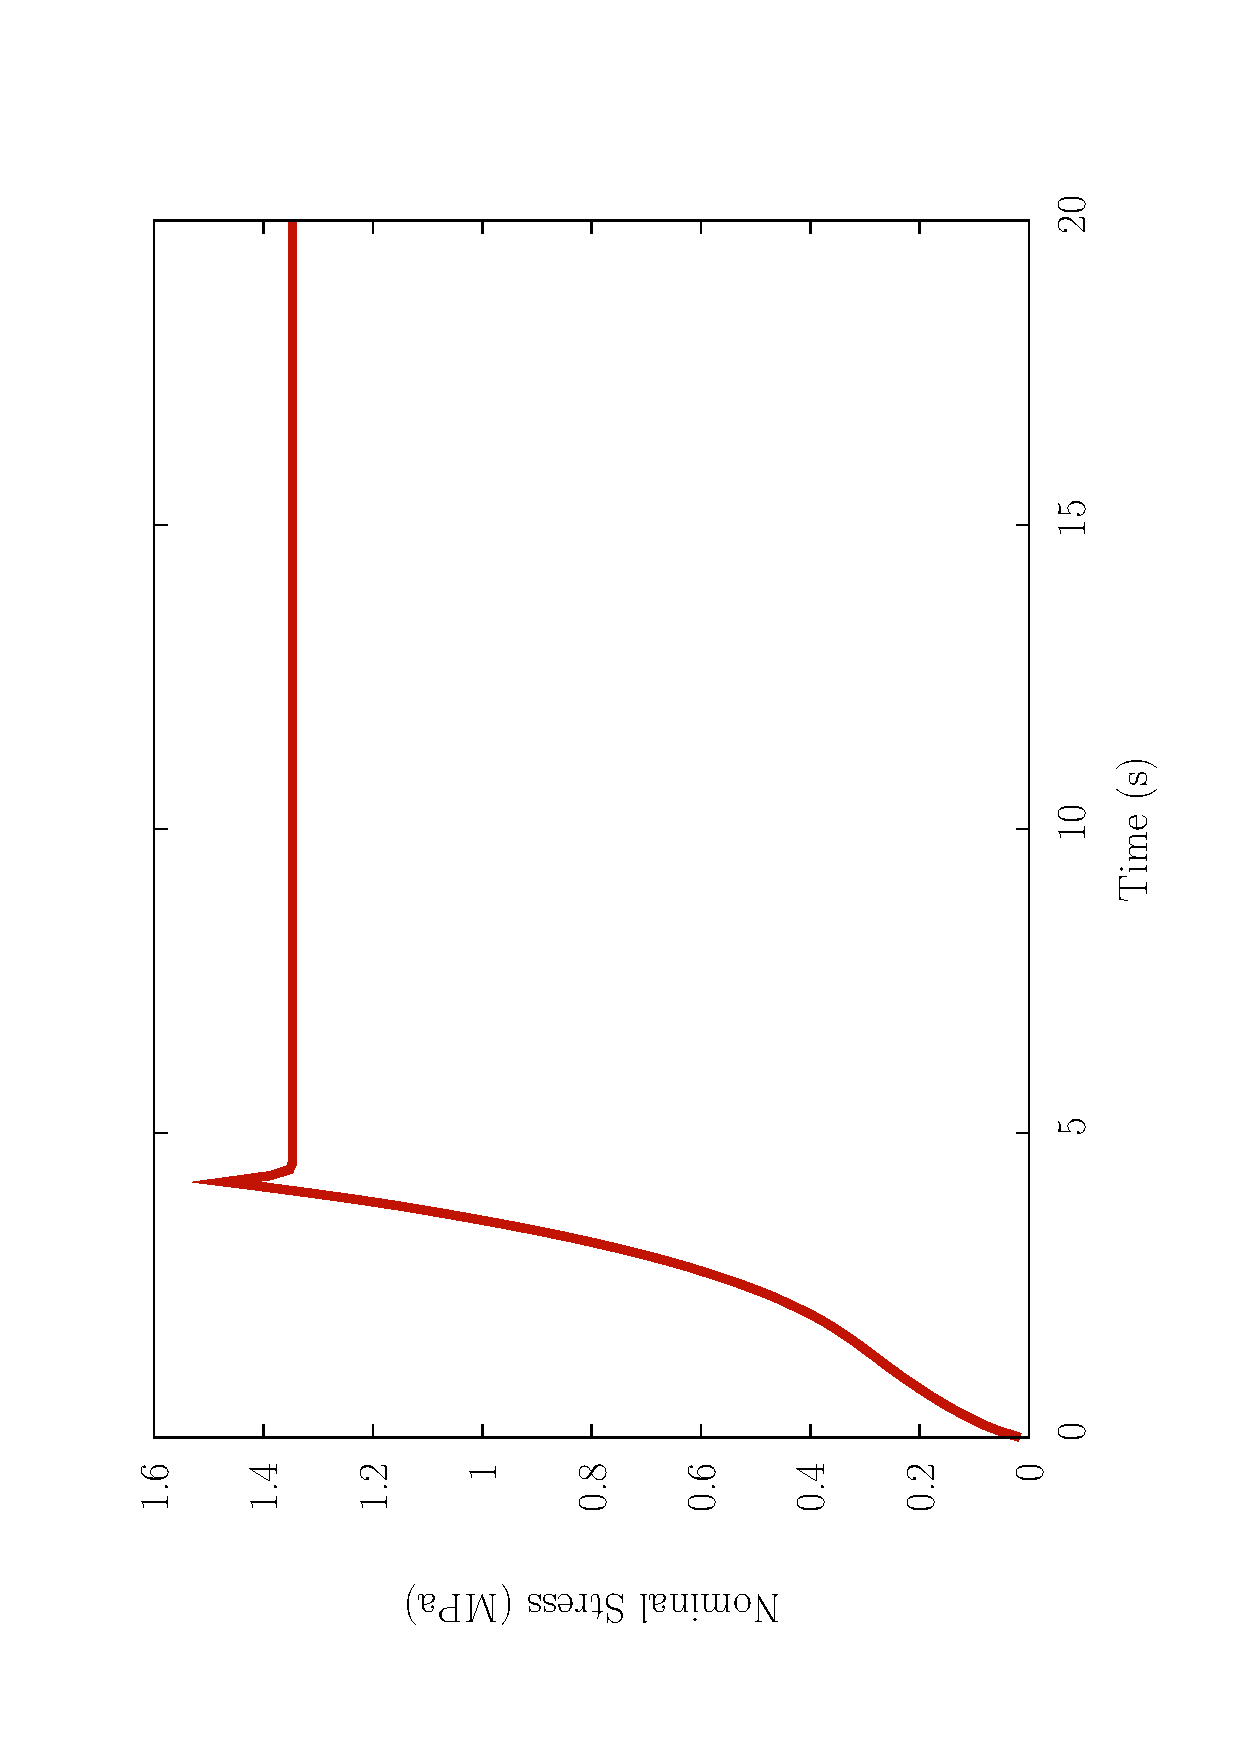
\includegraphics[width=0.6\textwidth,angle=270]{images/examples/%
eulerian/pulling/plots/poro-elastic/poro-stress-relax-0p02}
\caption{Dynamic poroelastic model, $\dot{\epsilon}=0.02$ Hz, $D=1.037$
  MPa.s.mm$^{-1}$.}
\label{poro-stress-relax-0p02}
\end{figure}

\subsubsection{Comparison with representative linear viscoelastic
  curve}
\label{viscoelastic-stress-relaxation}

\begin{figure}[!hptb]
\centering
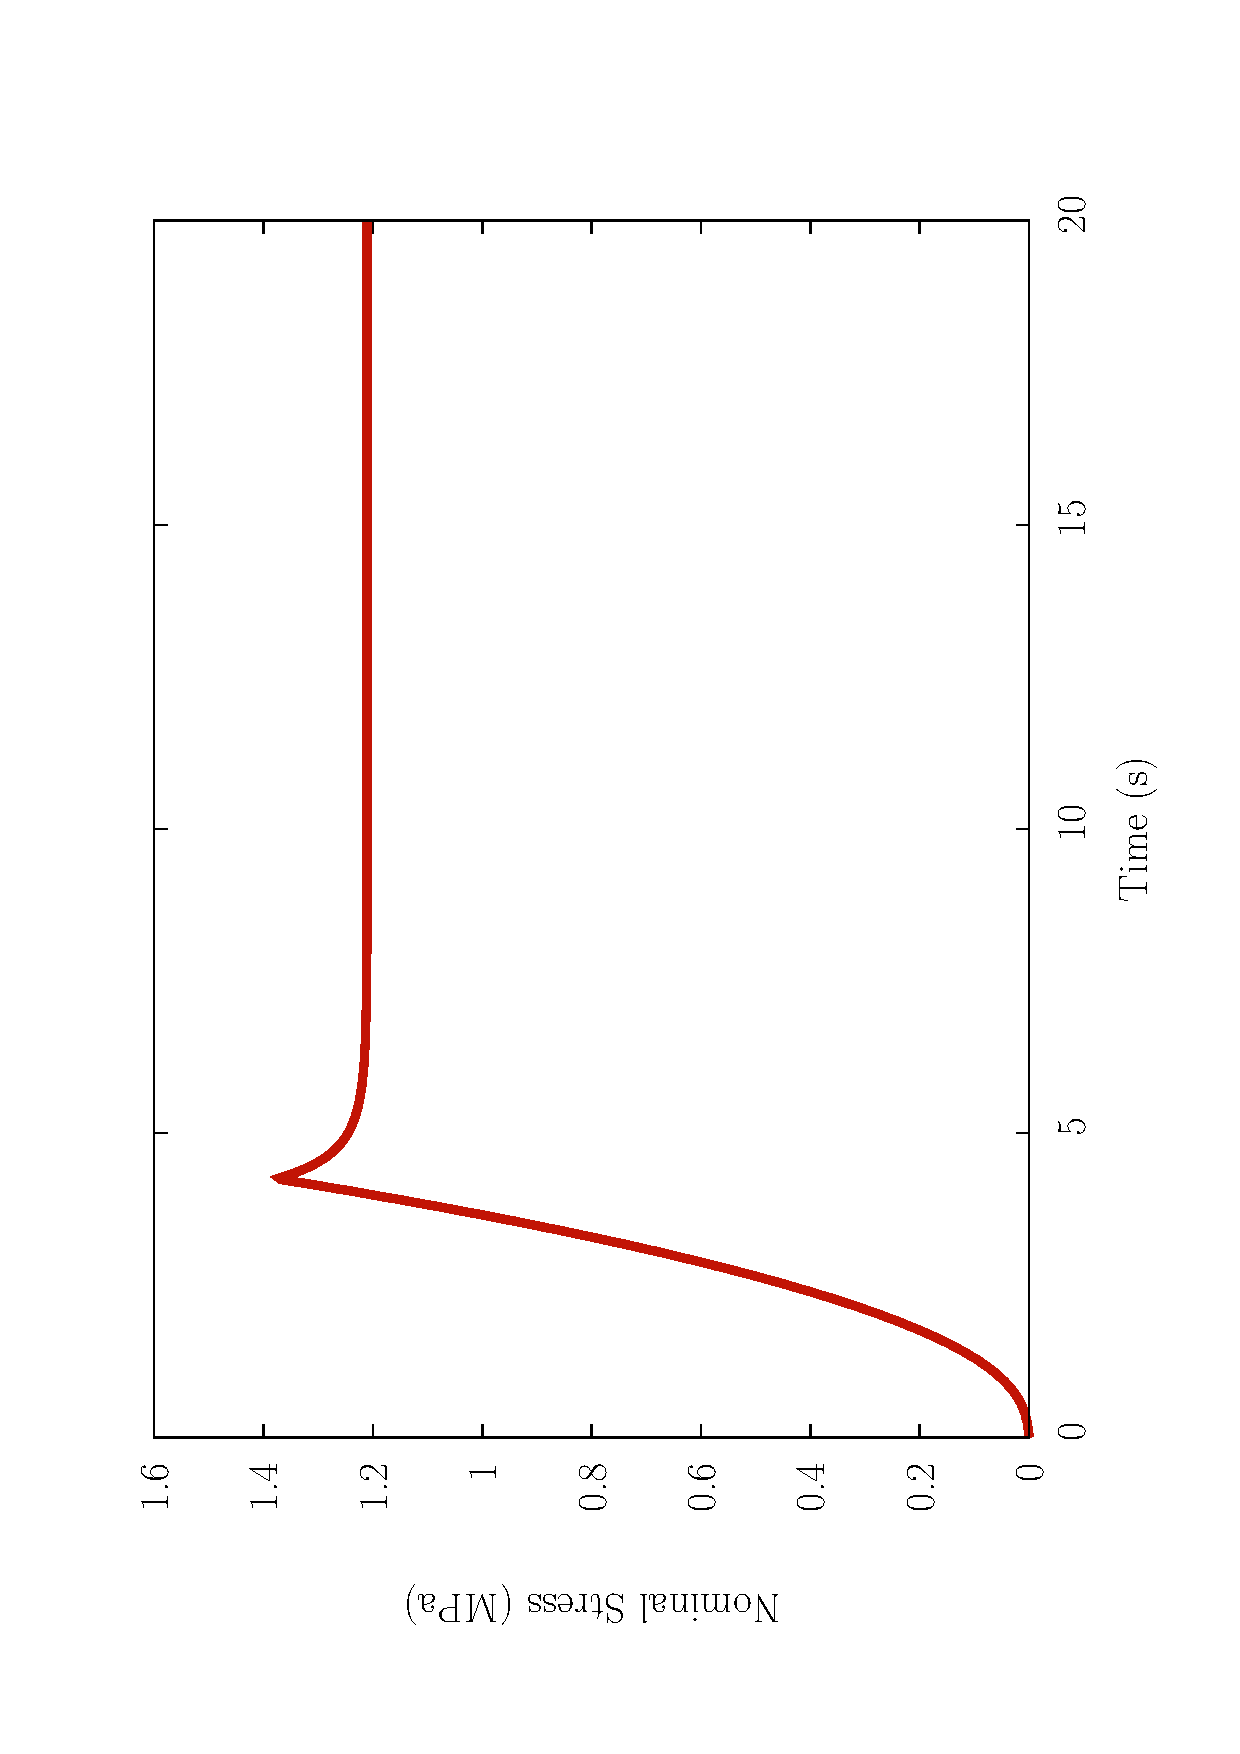
\includegraphics[width=0.6\textwidth,angle=270]{images/examples/%
eulerian/pulling/plots/visco-elastic/visco-stress-relax-0p02-t0p3}
\caption{Dynamic viscoelastic model, $\dot{\epsilon}=0.02$ Hz,
  $\tau=0.3$ s.}
\label{visco-stress-relax-0p02-t0p3}
\end{figure}

\subsection{Hysteresis in the cyclic stress-strain response}
\label{hysteresis}

\subsubsection{Quasistatic vs. dynamic}
\label{quasistatic-vs-dynamic}

\begin{figure}[!hptb]
\centering
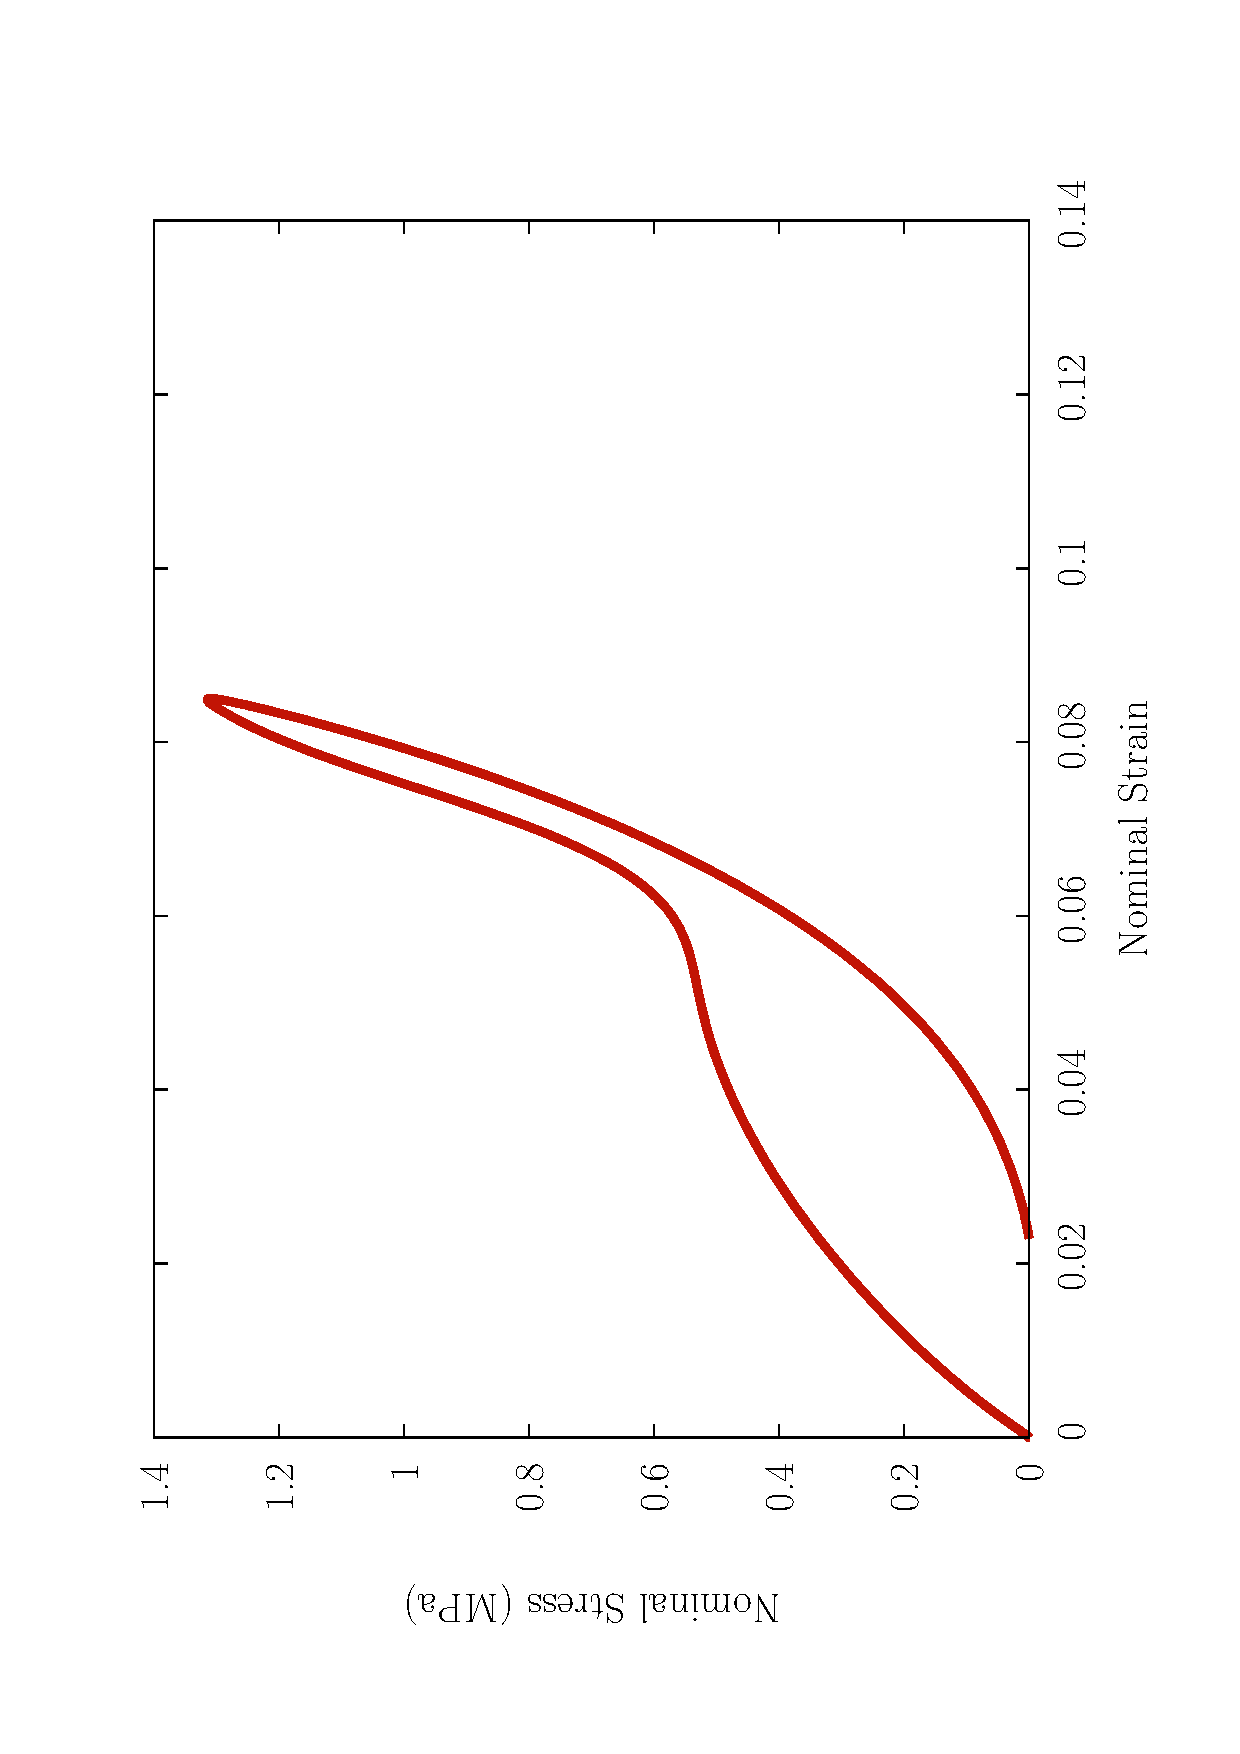
\includegraphics[width=0.6\textwidth,angle=270]{images/examples/%
eulerian/pulling/plots/poro-elastic/medium-hysteresis-dynamic-0p01-d1p037}
\caption{Dynamic poroelastic model, $\dot{\epsilon}=0.01$ Hz, $D=1.037$
  MPa.s.mm$^{-1}$.}
\label{medium-hysteresis-dynamic-0p01-d1p037}
\end{figure}

\begin{figure}[!hptb]
\centering
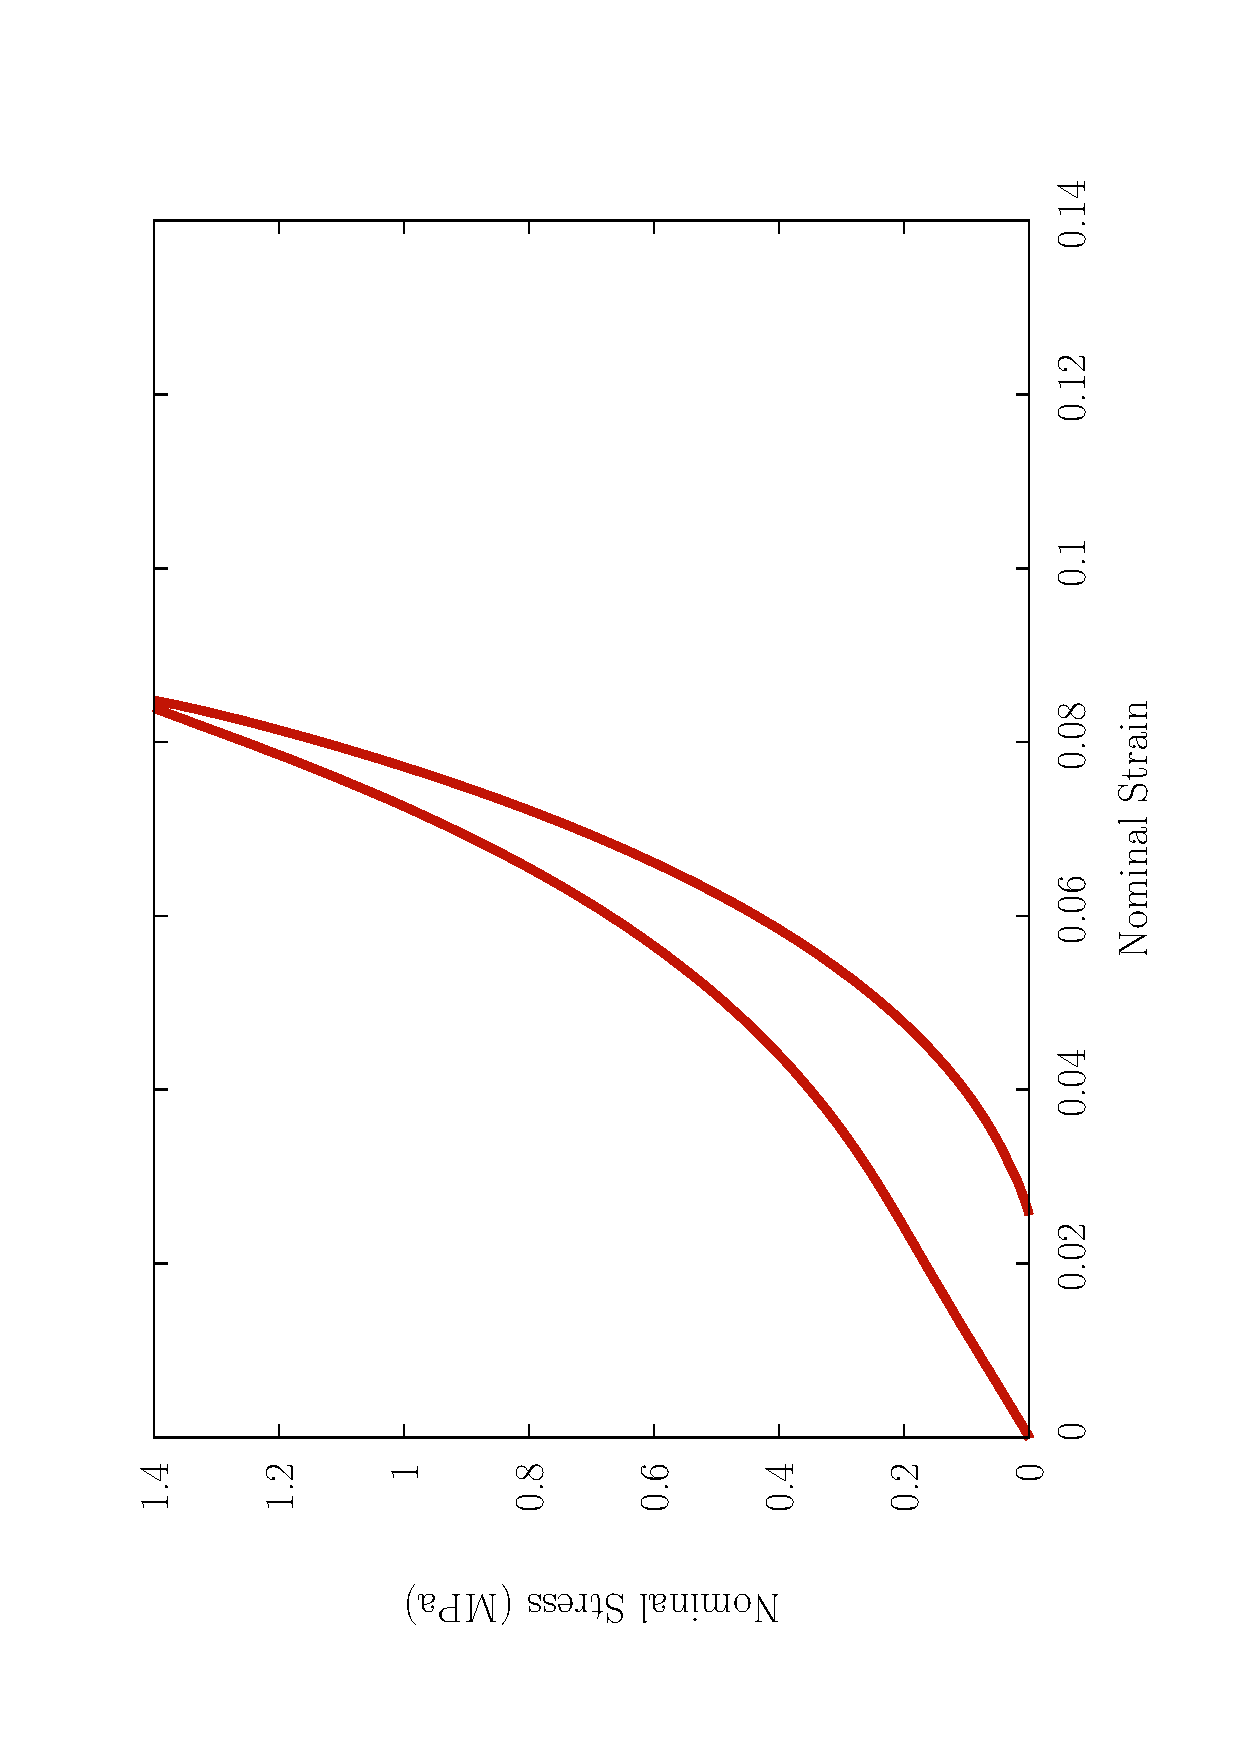
\includegraphics[width=0.6\textwidth,angle=270]{images/examples/%
eulerian/pulling/plots/poro-elastic/medium-hysteresis-static-0p01-d1p037}
\caption{Quasistatic poroelastic model, $\dot{\epsilon}=0.01$ Hz, $D=1.037$
  MPa.s.mm$^{-1}$.}
\label{medium-hysteresis-static-0p01-d1p037}
\end{figure}

\subsubsection{Changing load-rates and friction coefficients}
\label{load-rates-and-friction-coefficients}

\begin{figure}[!hptb]
\centering
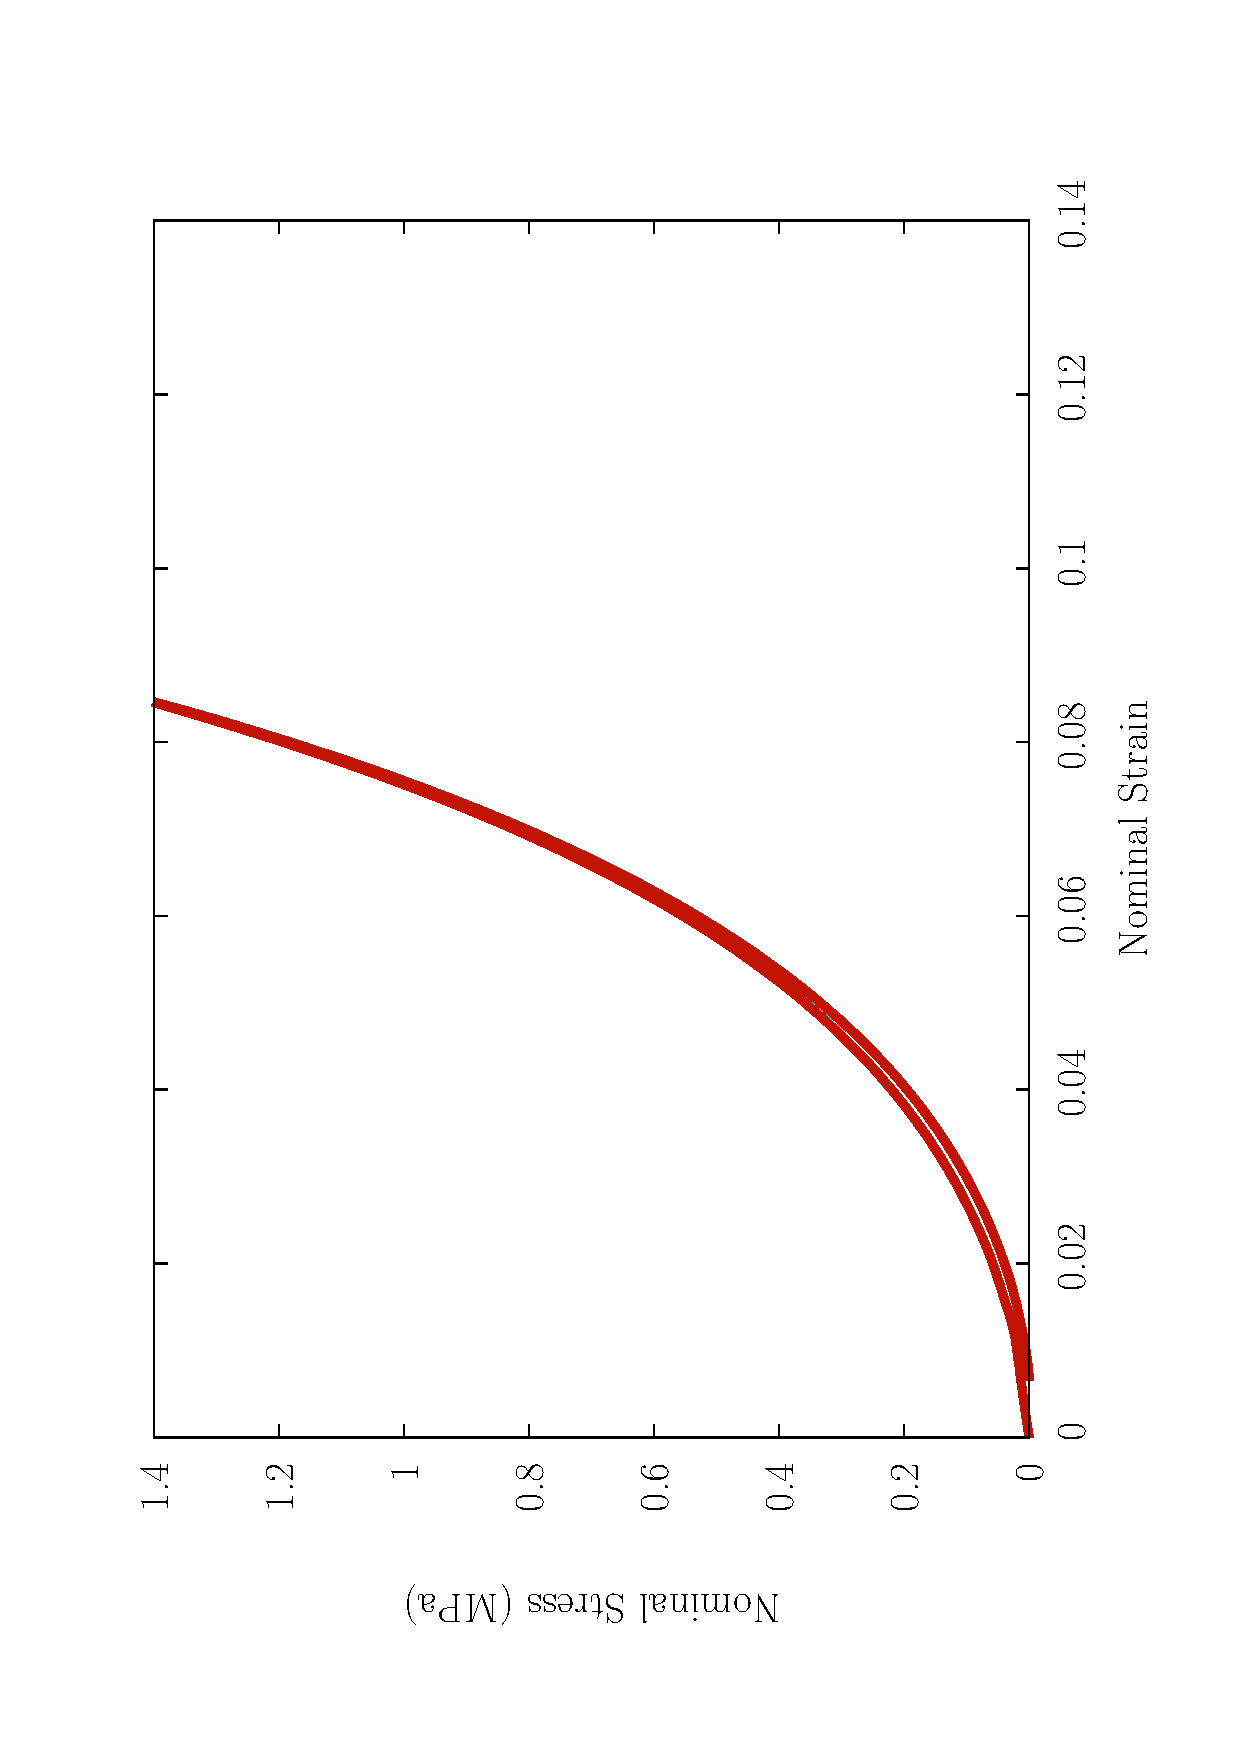
\includegraphics[width=0.6\textwidth,angle=270]{images/examples/%
eulerian/pulling/plots/poro-elastic/medium-hysteresis-dynamic-0p001-d1p037}
\caption{Dynamic poroelastic model, $\dot{\epsilon}=0.001$ Hz, $D=1.037$
  MPa.s.mm$^{-1}$.}
\label{medium-hysteresis-dynamic-0p001-d1p037}
\end{figure}

\begin{figure}[!hptb]
\centering
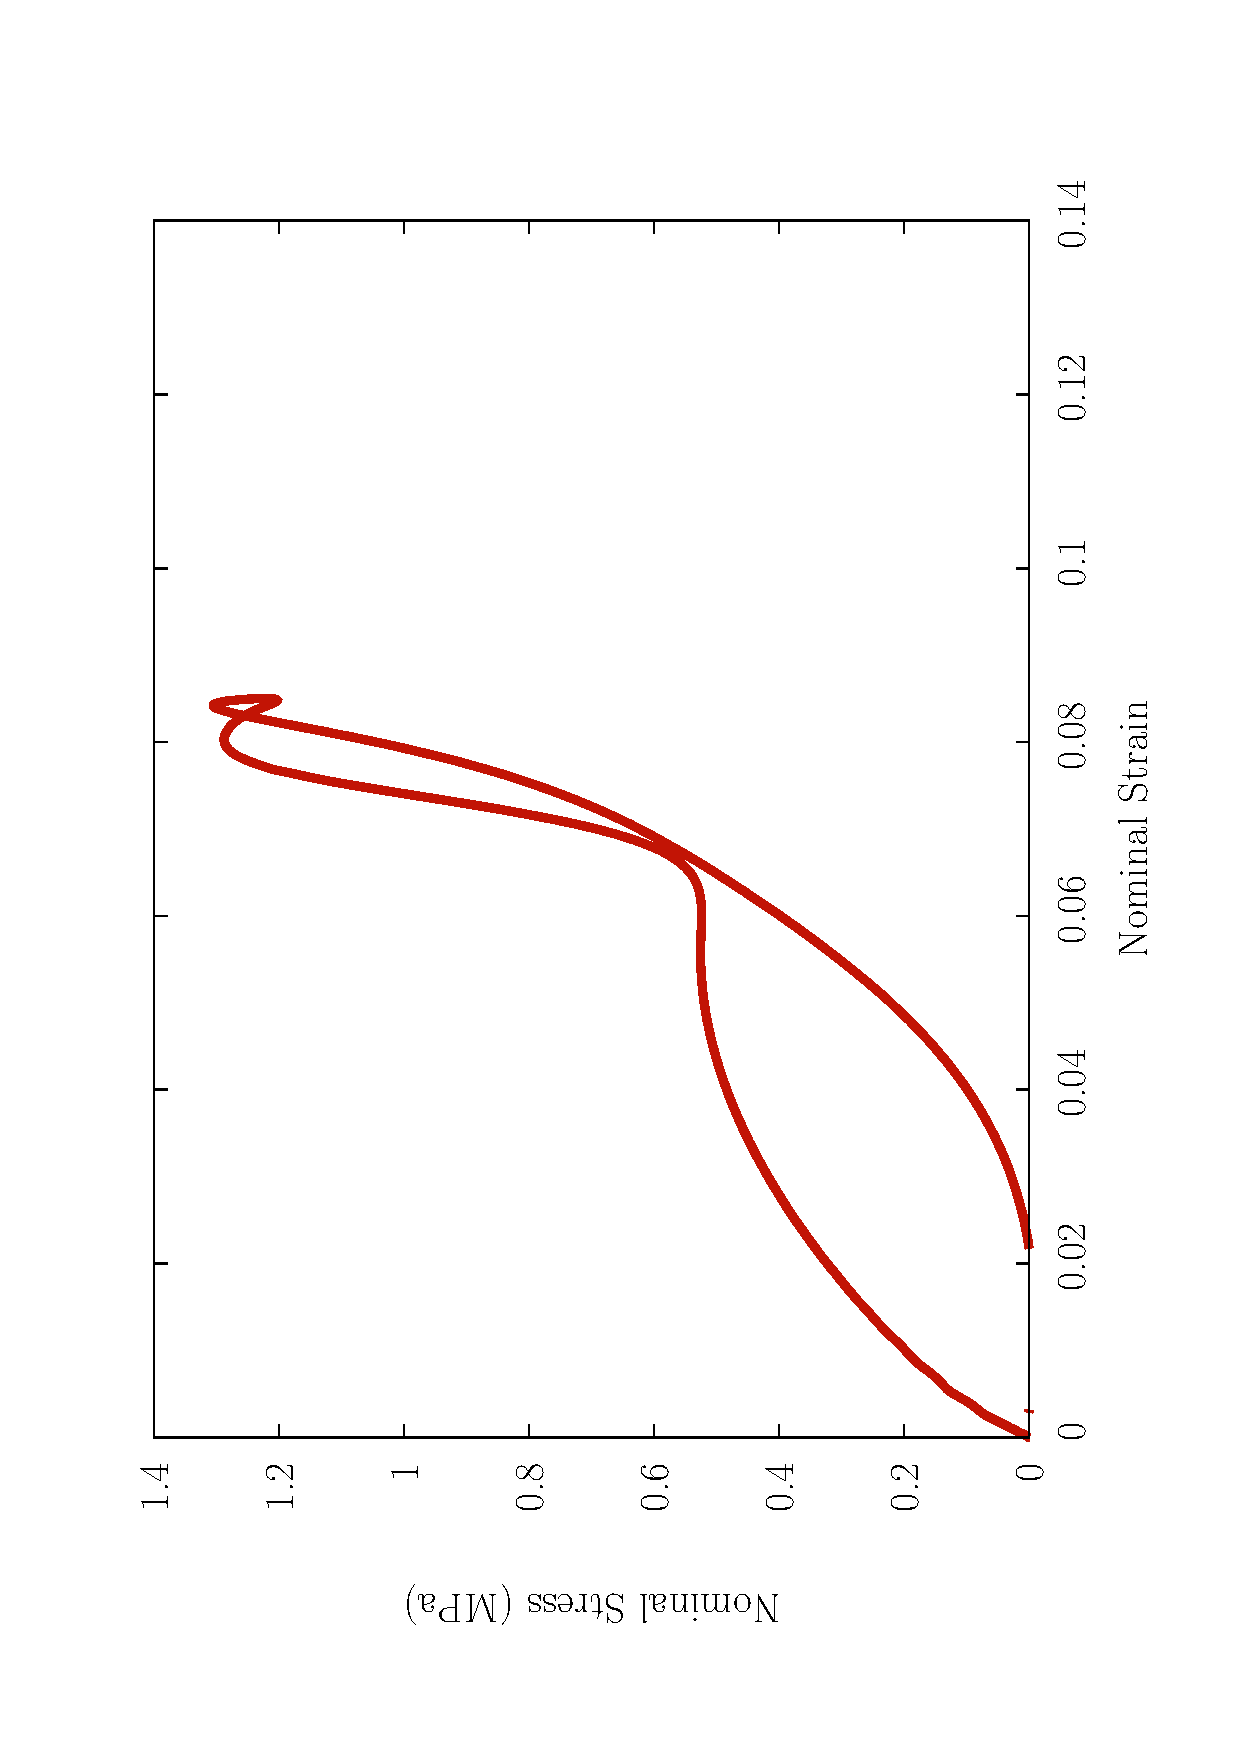
\includegraphics[width=0.6\textwidth,angle=270]{images/examples/%
eulerian/pulling/plots/poro-elastic/medium-hysteresis-dynamic-0p01-d10p37}
\caption{Dynamic poroelastic model, $\dot{\epsilon}=0.01$ Hz, $D=10.37$
  MPa.s.mm$^{-1}$.}
\label{medium-hysteresis-dynamic-0p01-d10p37}
\end{figure}

\subsubsection{Changing the overall shape and stress range}
\label{changing-shape}

\begin{figure}[!hptb]
\centering
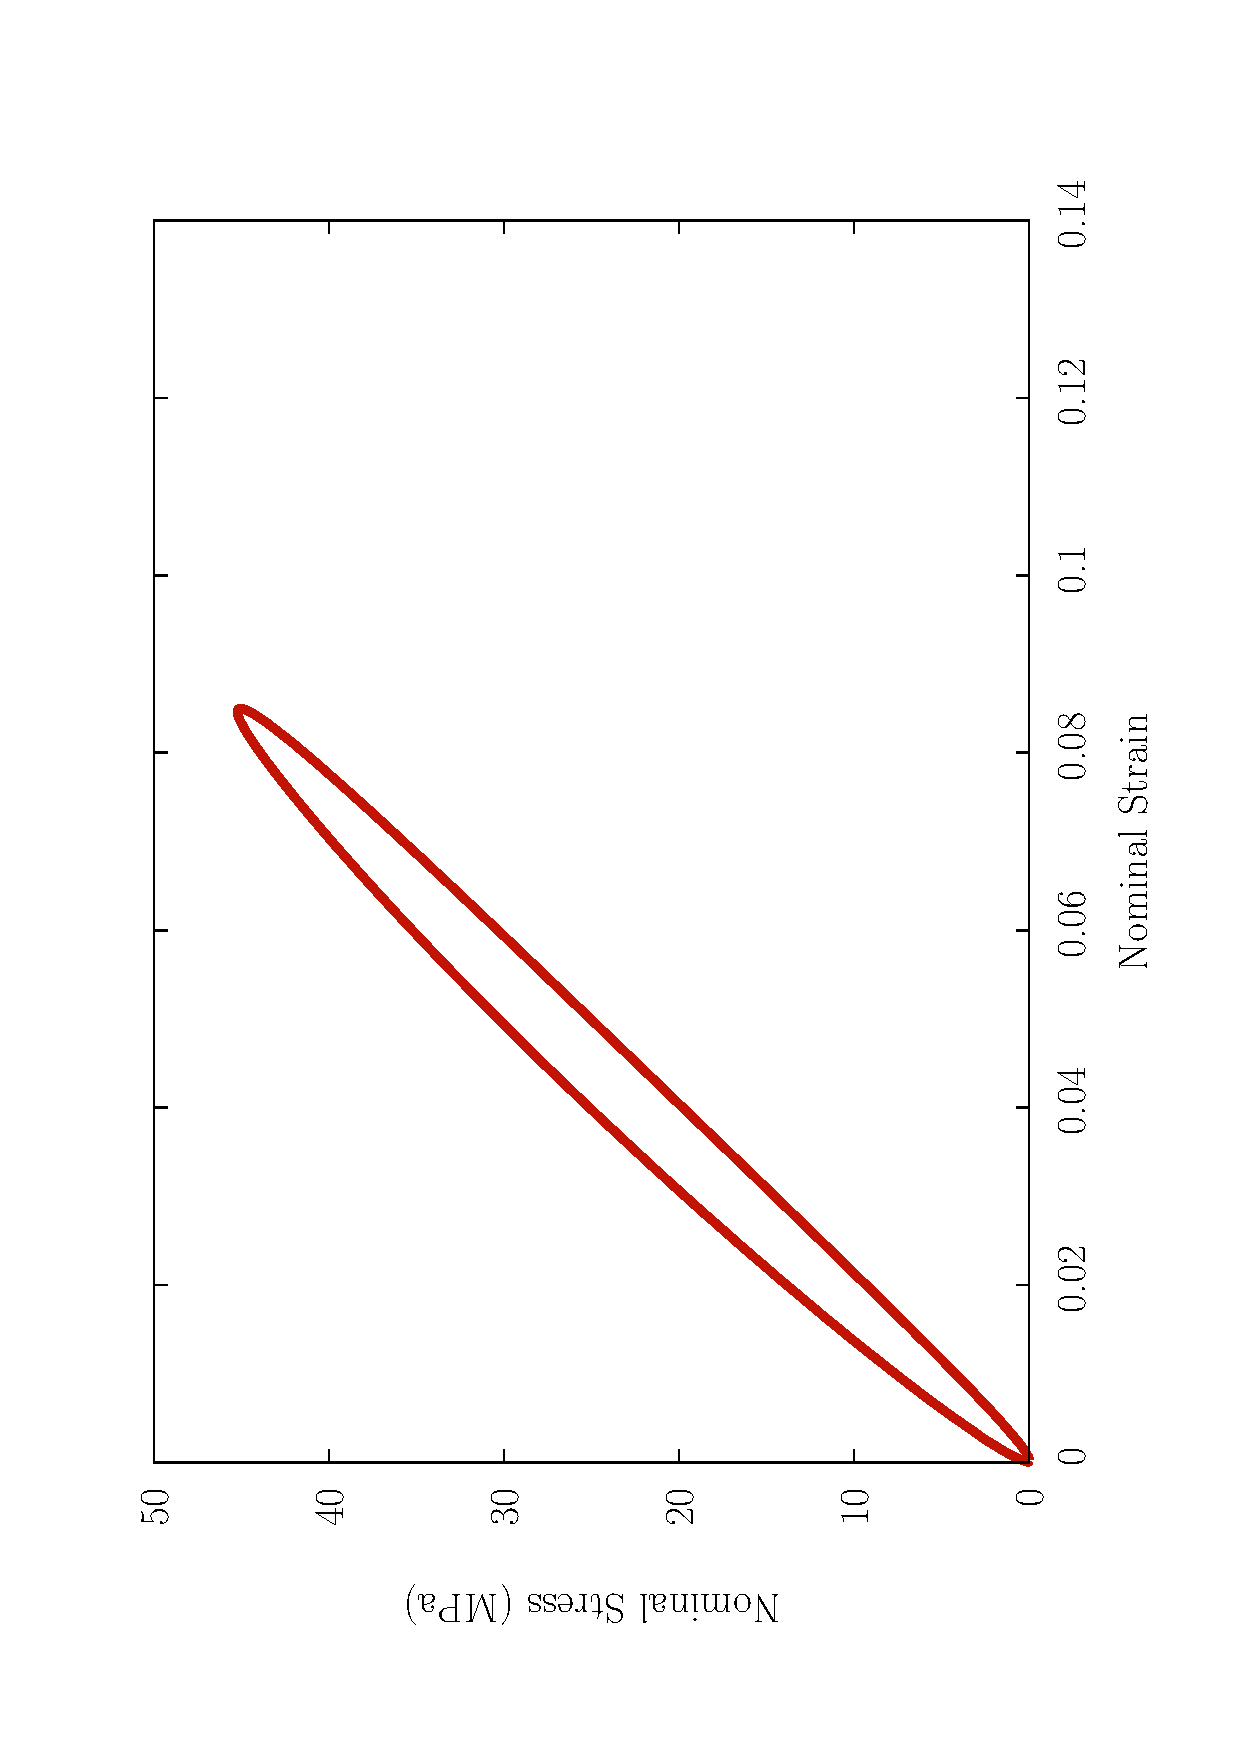
\includegraphics[width=0.6\textwidth,angle=270]{images/examples/%
eulerian/pulling/plots/poro-elastic/low-hysteresis-dynamic-0p01-d1p037}
\caption{Dynamic poroelastic model, $\dot{\epsilon}=0.01$ Hz, $D=1.037$
  MPa.s.mm$^{-1}$.}
\label{low-hysteresis-dynamic-0p01-d1p037}
\end{figure}

\subsubsection{Comparison with representative linear viscoelastic
  curves}
\label{viscoelastic-hysteresis}

\begin{figure}[!hptb]
\centering
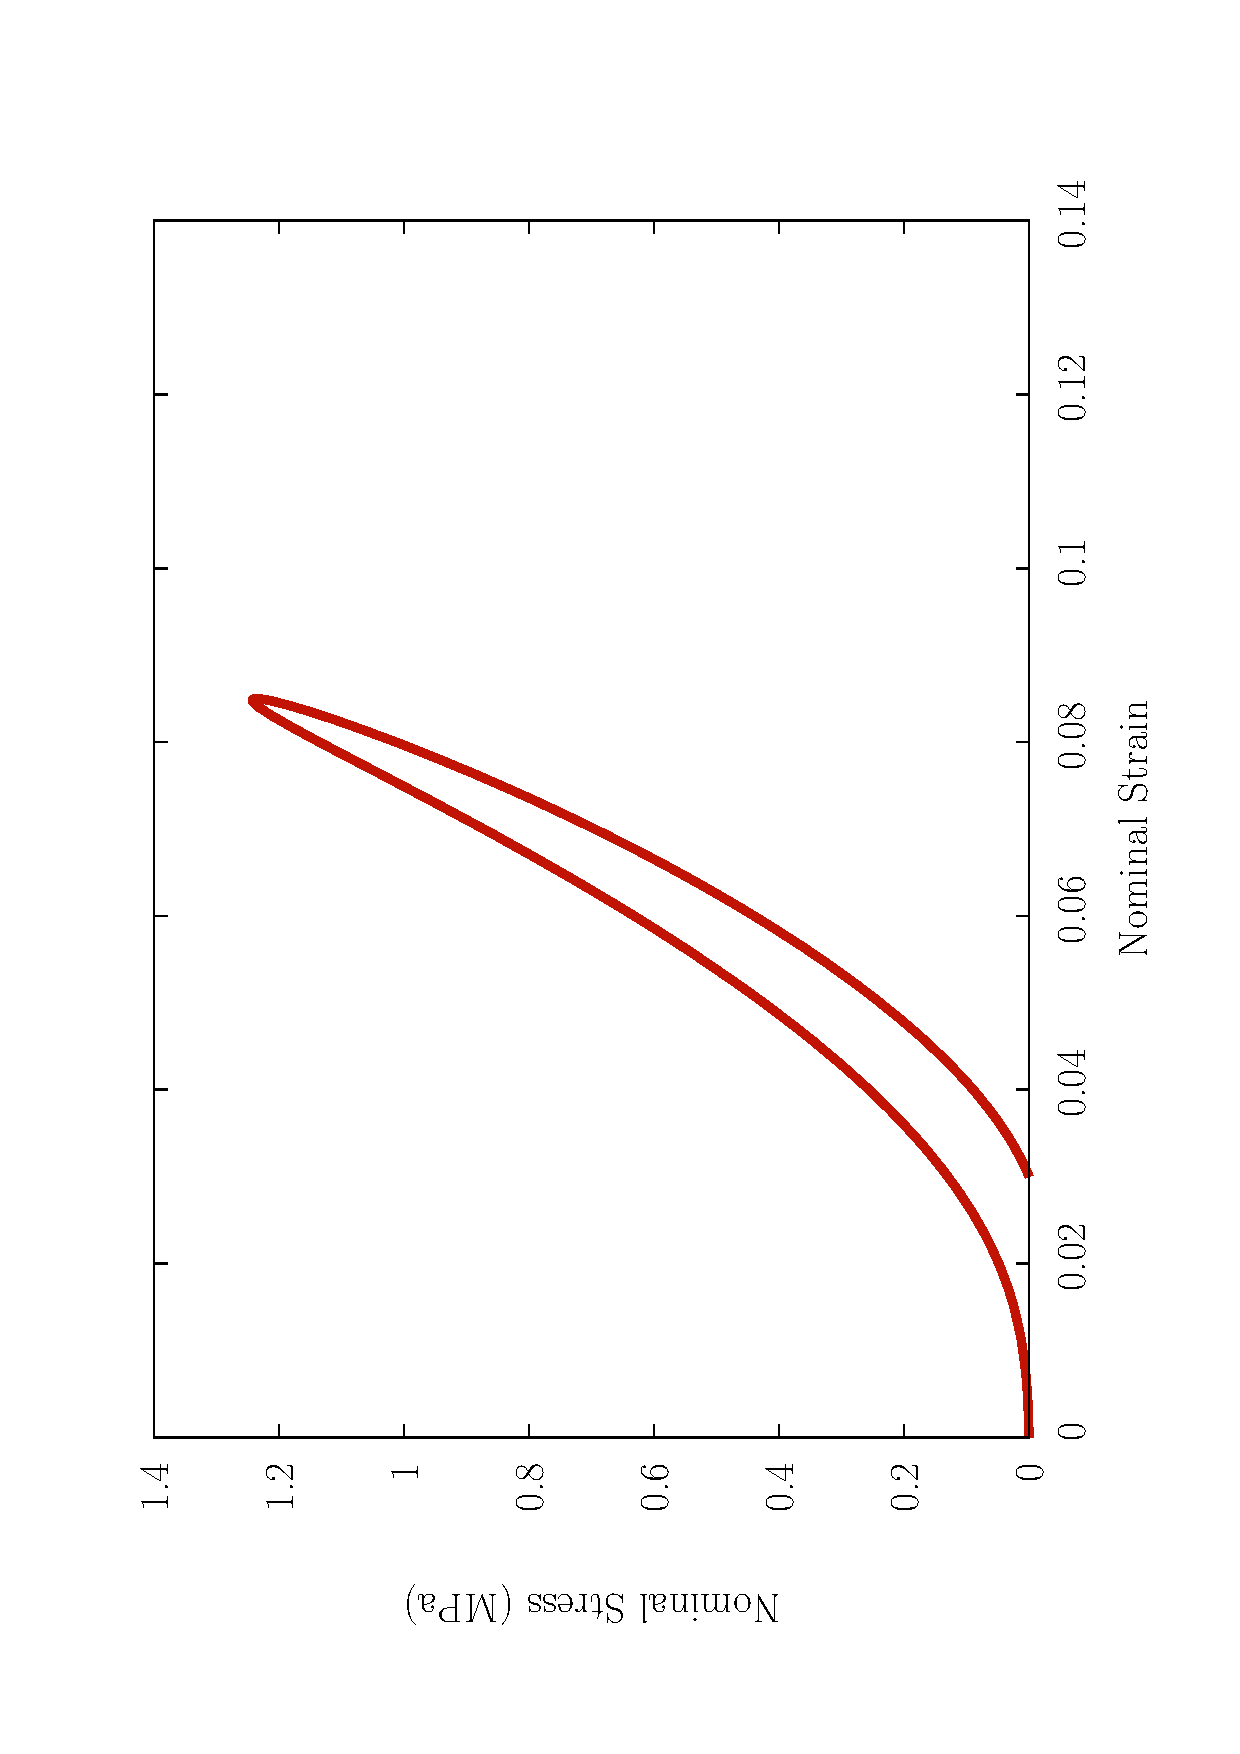
\includegraphics[width=0.6\textwidth,angle=270]{images/examples/%
eulerian/pulling/plots/visco-elastic/medium-hysteresis-visco-0p01-t0p3}
\caption{Dynamic viscoelastic model, $\dot{\epsilon}=0.01$ Hz,
  $\tau=0.3$ s.}
\label{medium-hysteresis-visco-0p01-t0p3}
\end{figure}

\begin{figure}[!hptb]
\centering
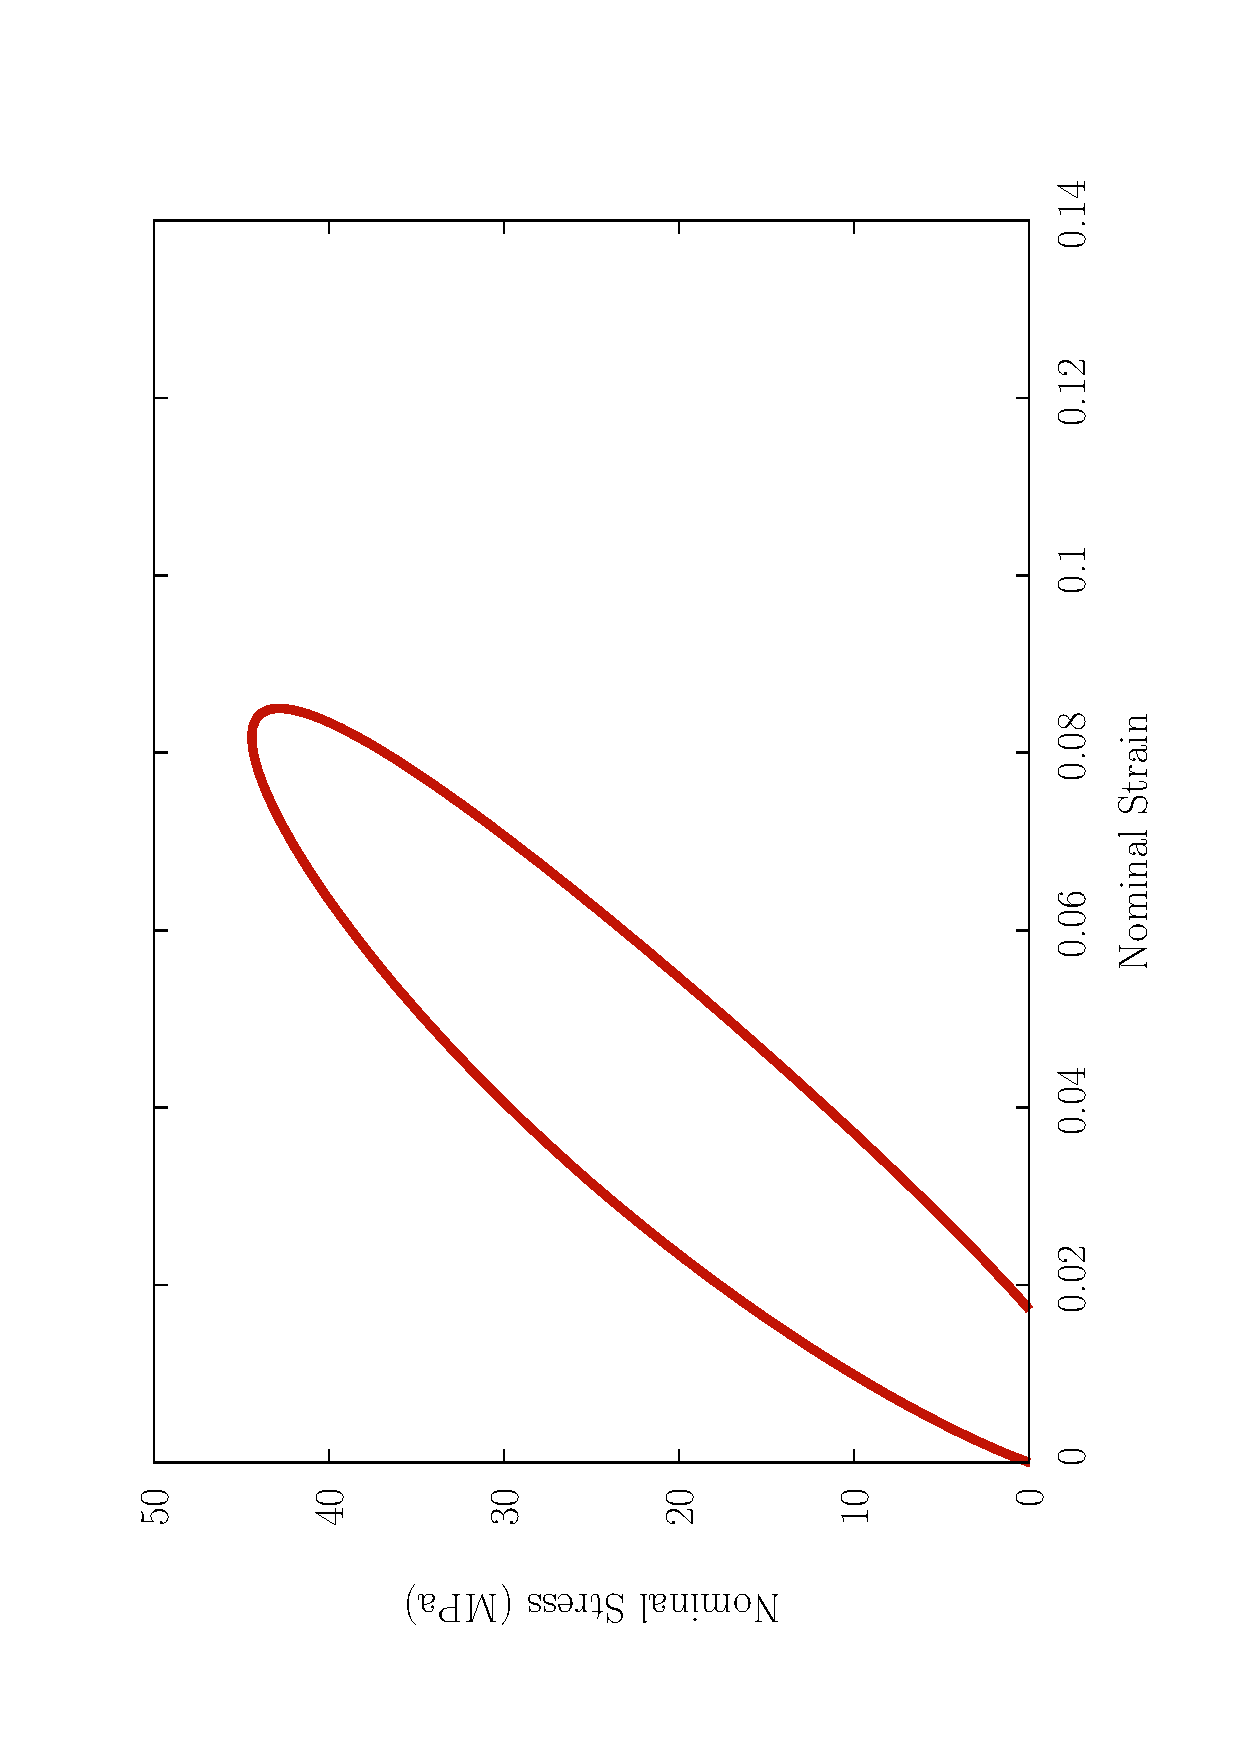
\includegraphics[width=0.6\textwidth,angle=270]{images/examples/%
eulerian/pulling/plots/visco-elastic/low-hysteresis-visco-0p01-t0p7}
\caption{Dynamic viscoelastic model, $\dot{\epsilon}=0.01$ Hz,
  $\tau=0.7$ s.}
\label{low-hysteresis-visco-0p01-t0p7}
\end{figure}

\section{Material modelling}
\label{material-modelling}

\subsection{Non-linear viscoelasticity}
\label{non-linear-viscoelasticity}

\begin{figure}[!hptb]
\centering
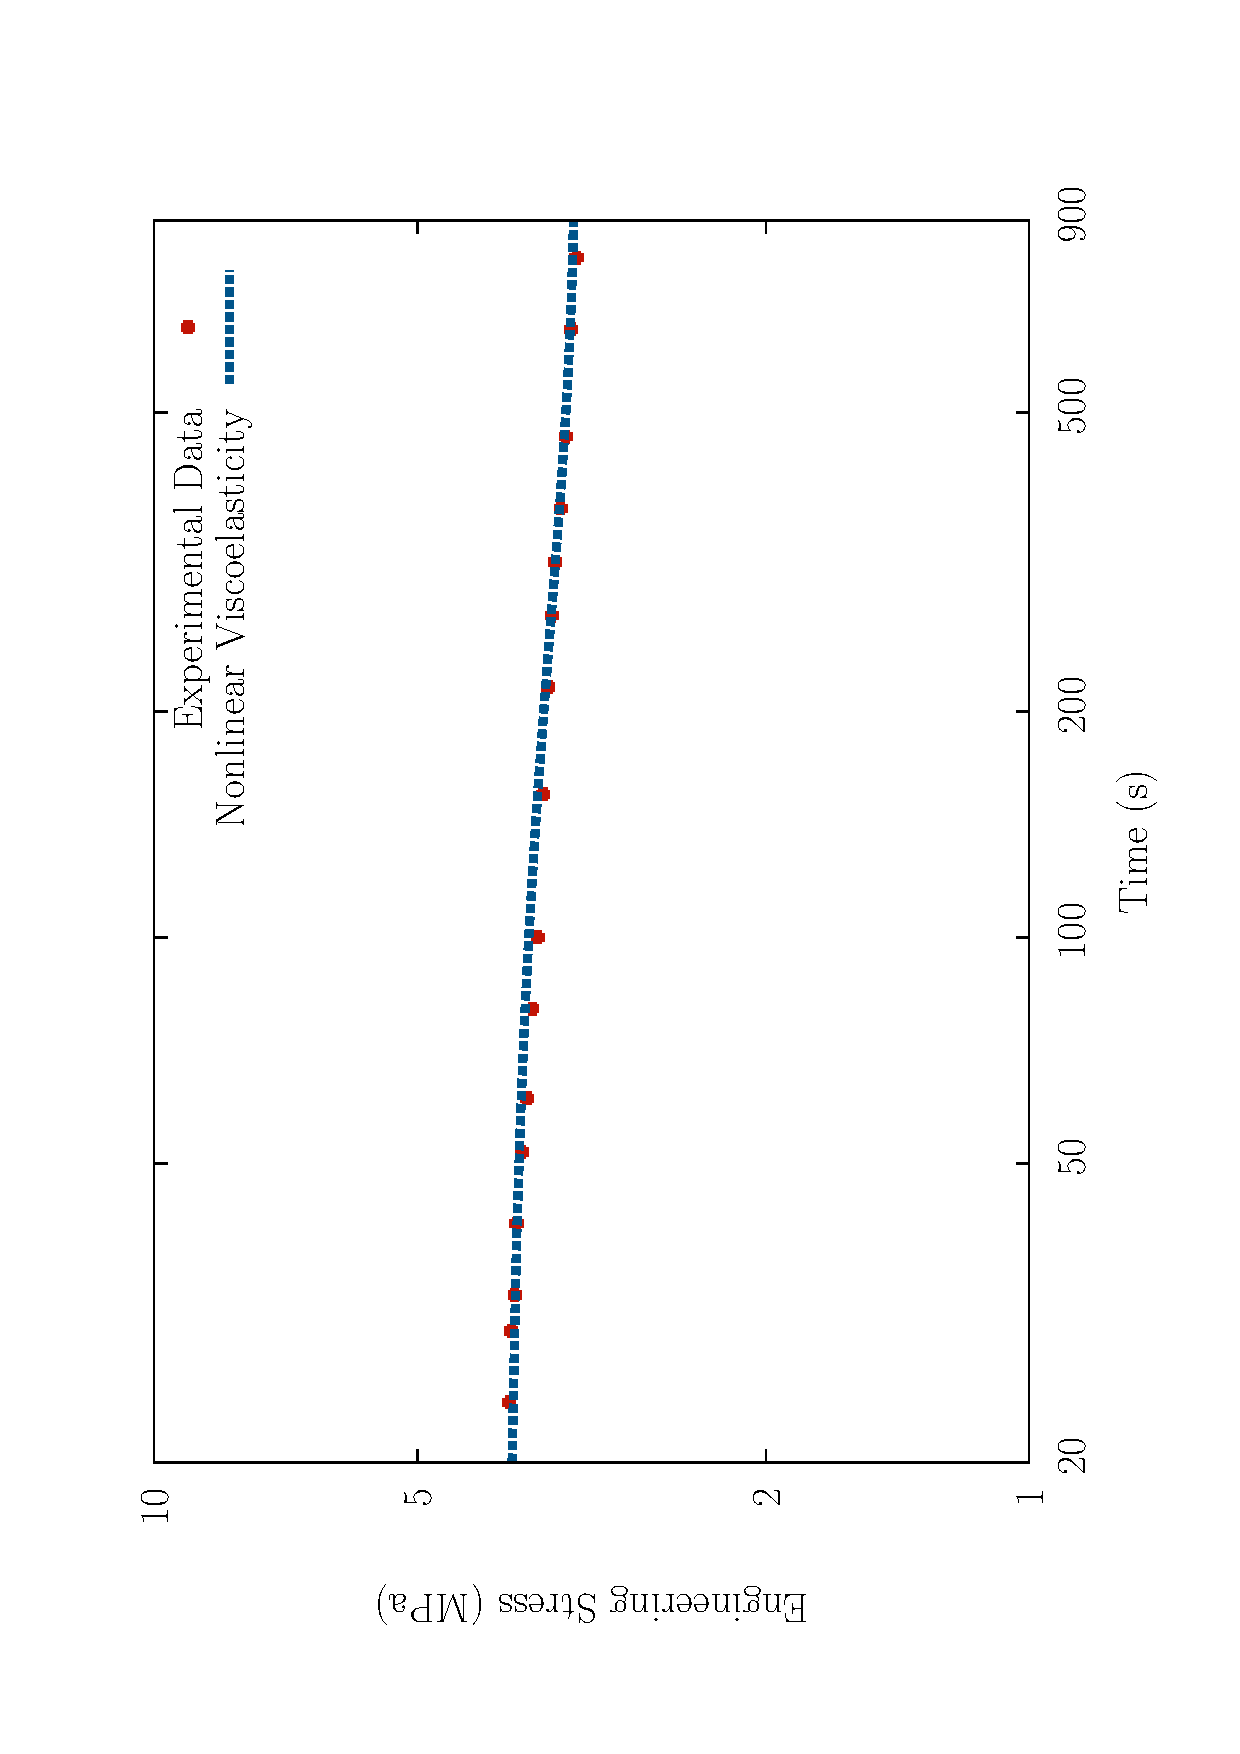
\includegraphics[width=0.6\textwidth,angle=270]{images/examples/%
eulerian/nonlinear-viscoelasticity/provenzano-data-comparison}
\caption{The non-linear time constants fit to experiment.} 
\label{provenzano-data-fit}
\end{figure}

\begin{figure}[!hptb]
\centering
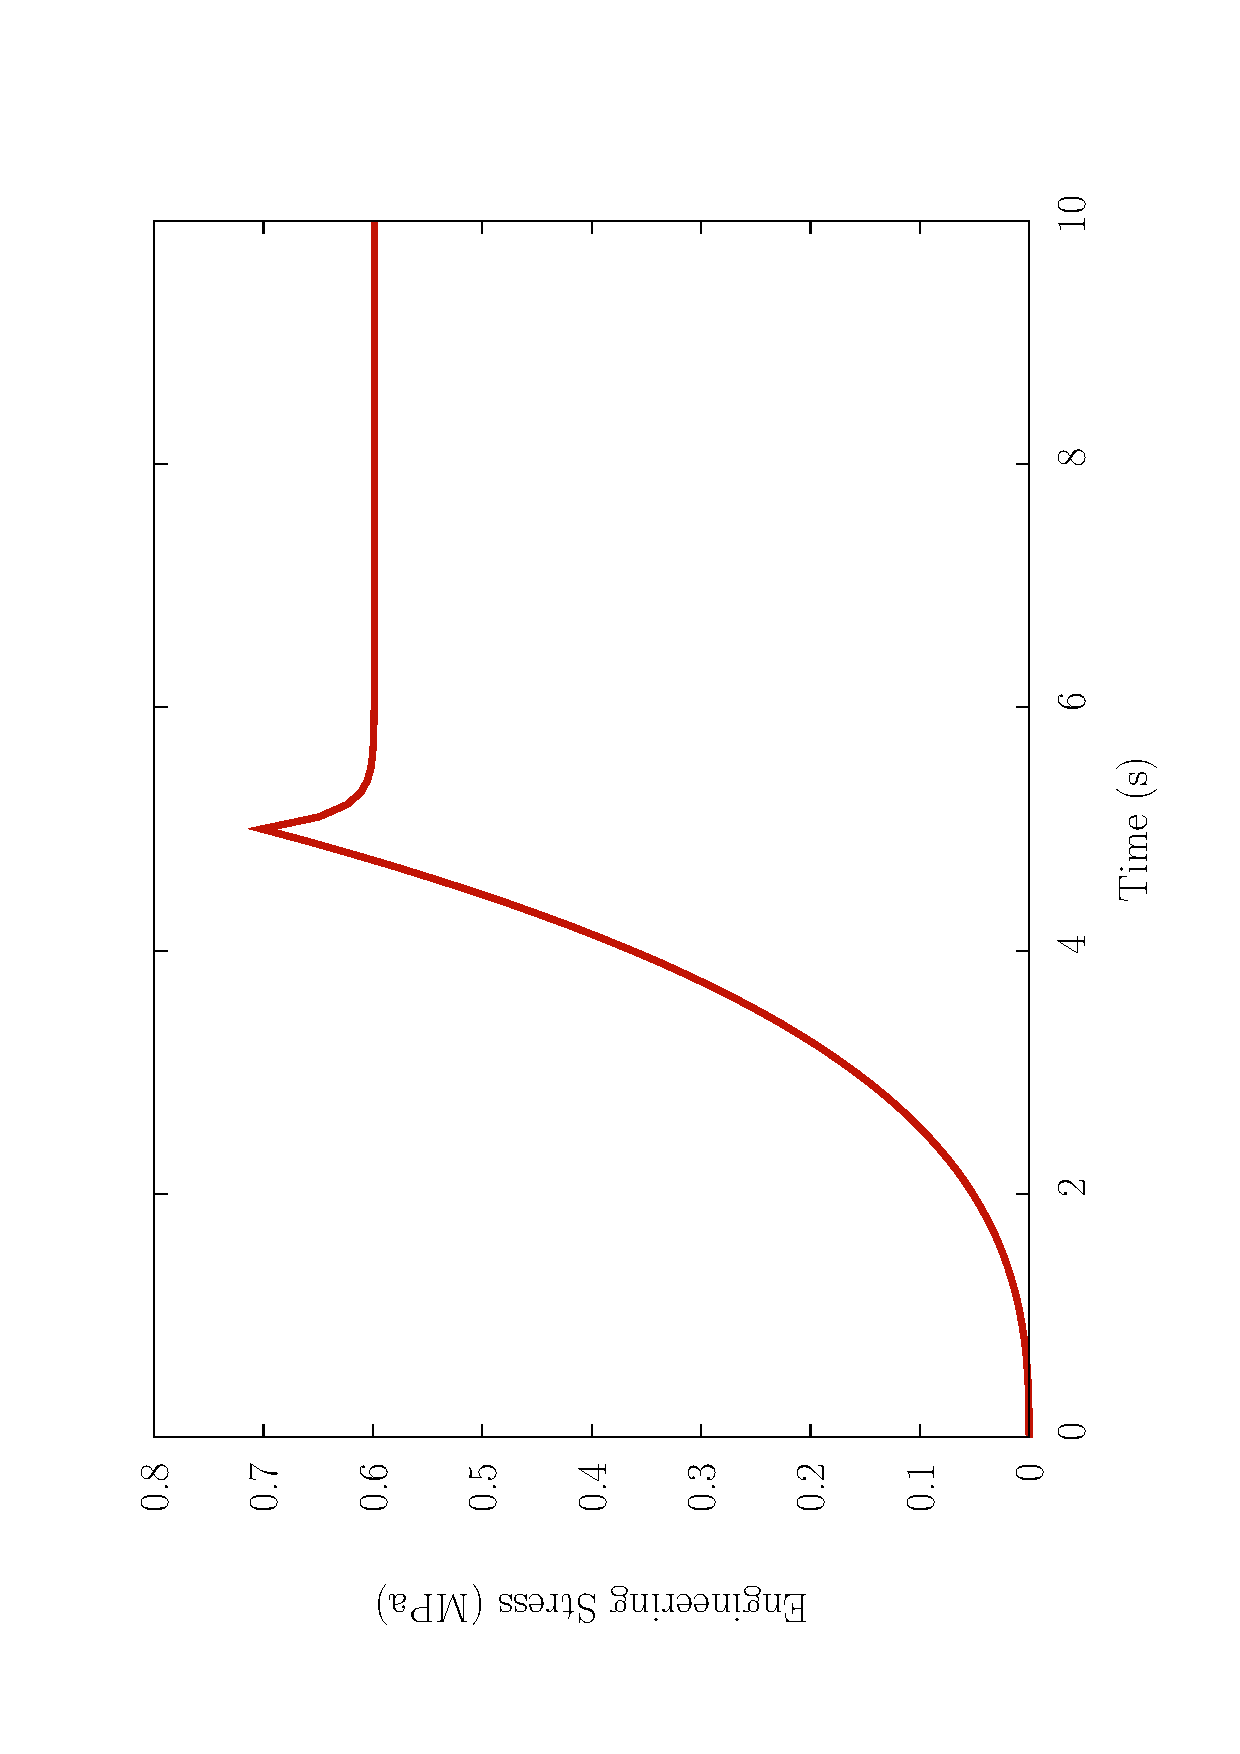
\includegraphics[width=0.6\textwidth,angle=270]{images/examples/%
eulerian/nonlinear-viscoelasticity/nonlinear-viscoelasticity-stress-relaxation}
\caption{Stress relaxation under nonlinear viscoelasticity.}
\label{nonlinear-viscoelasticity-stress-relaxation}
\end{figure}

\subsection{Friction coefficient variation with concentration}
\label{variable-friction-coefficient}

\section{Tumour growth}
\label{tumour-growth}

\subsection{Isotropic swelling}
\label{tumour-isotropic-swelling}

\begin{figure}[!hptb]
\centering
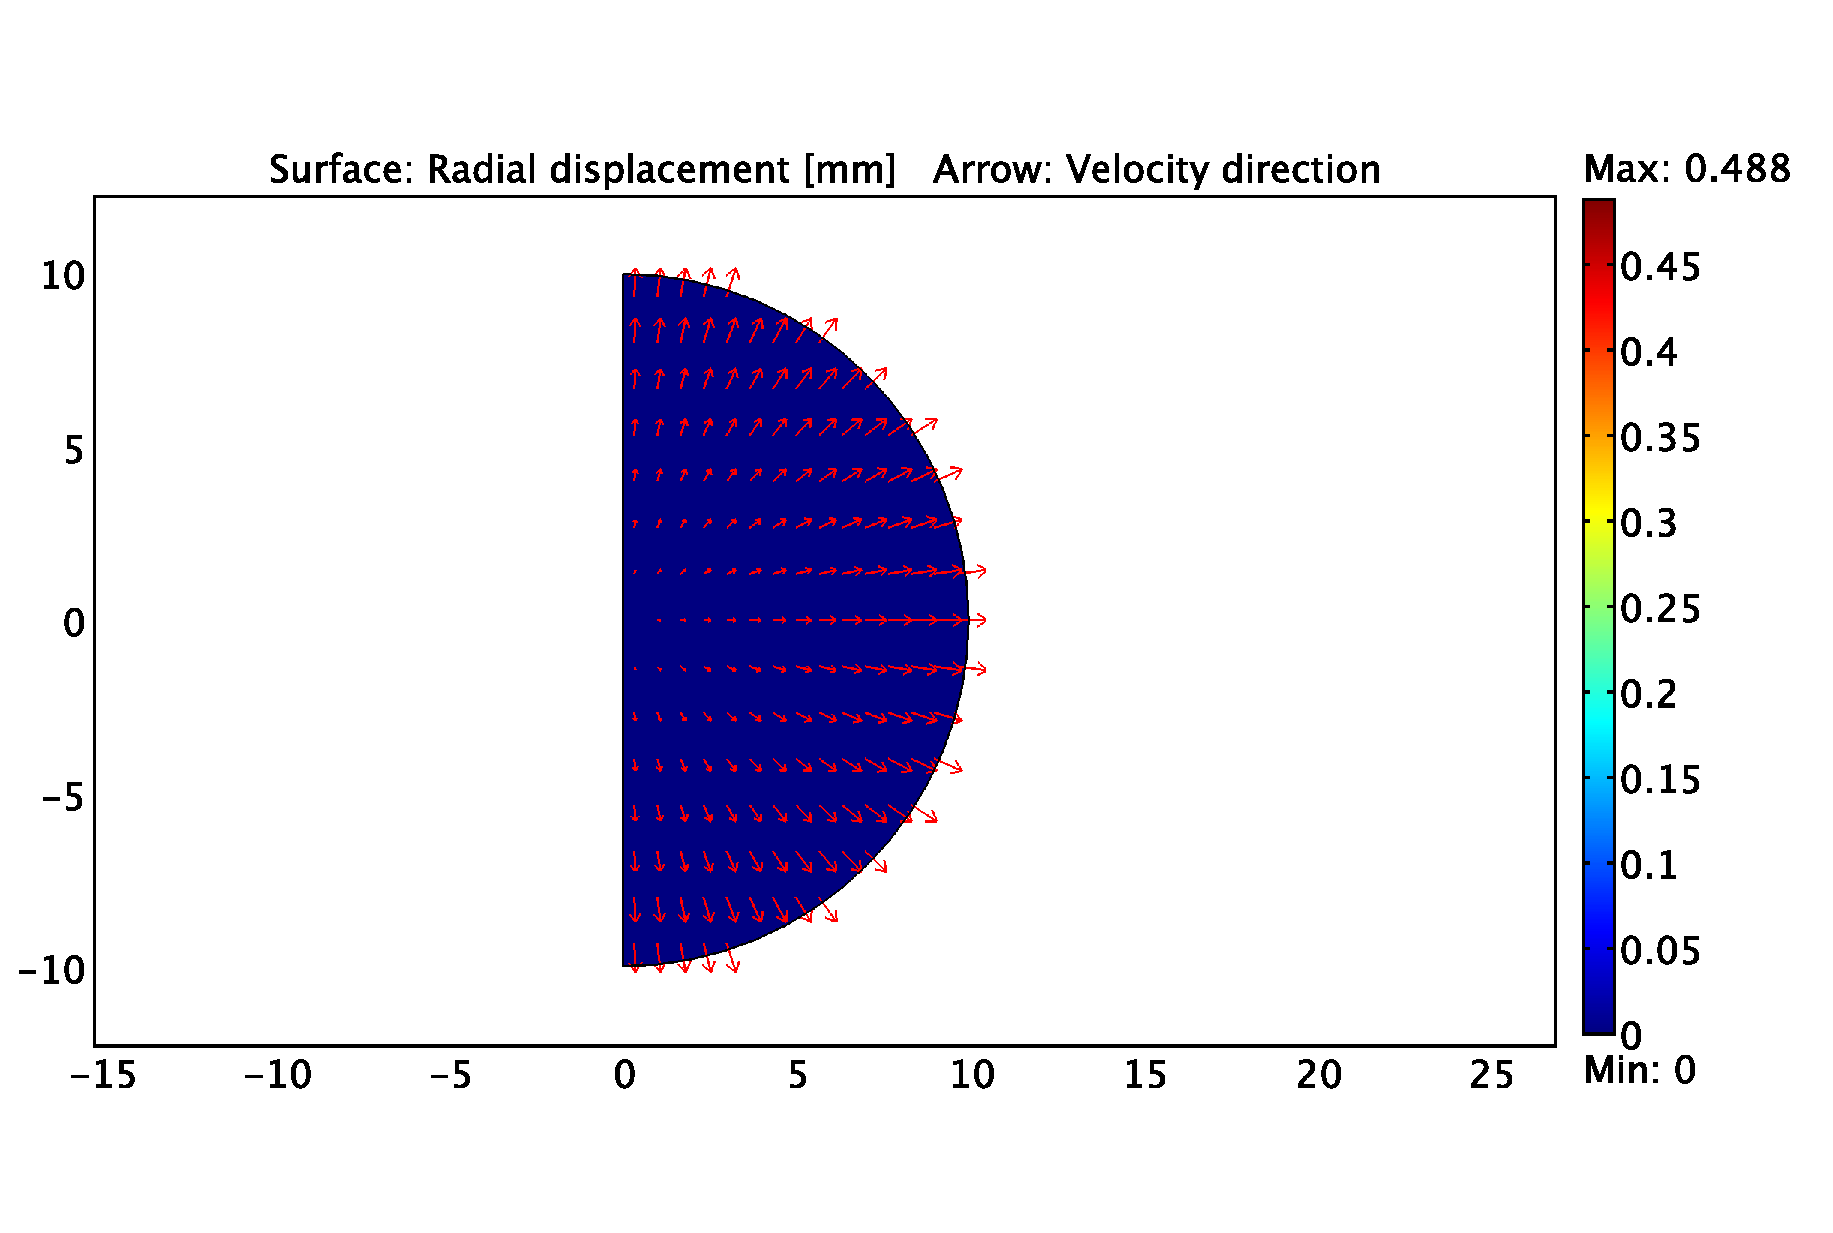
\includegraphics[width=0.8\textwidth]{images/examples/%
eulerian/cancer/isotropic-swelling-0}
\caption{A semicircular tumour at time $t=0$ days.}
\label{tumour-isotropic-swelling-0}
\end{figure}

\begin{figure}[!hptb]
\centering
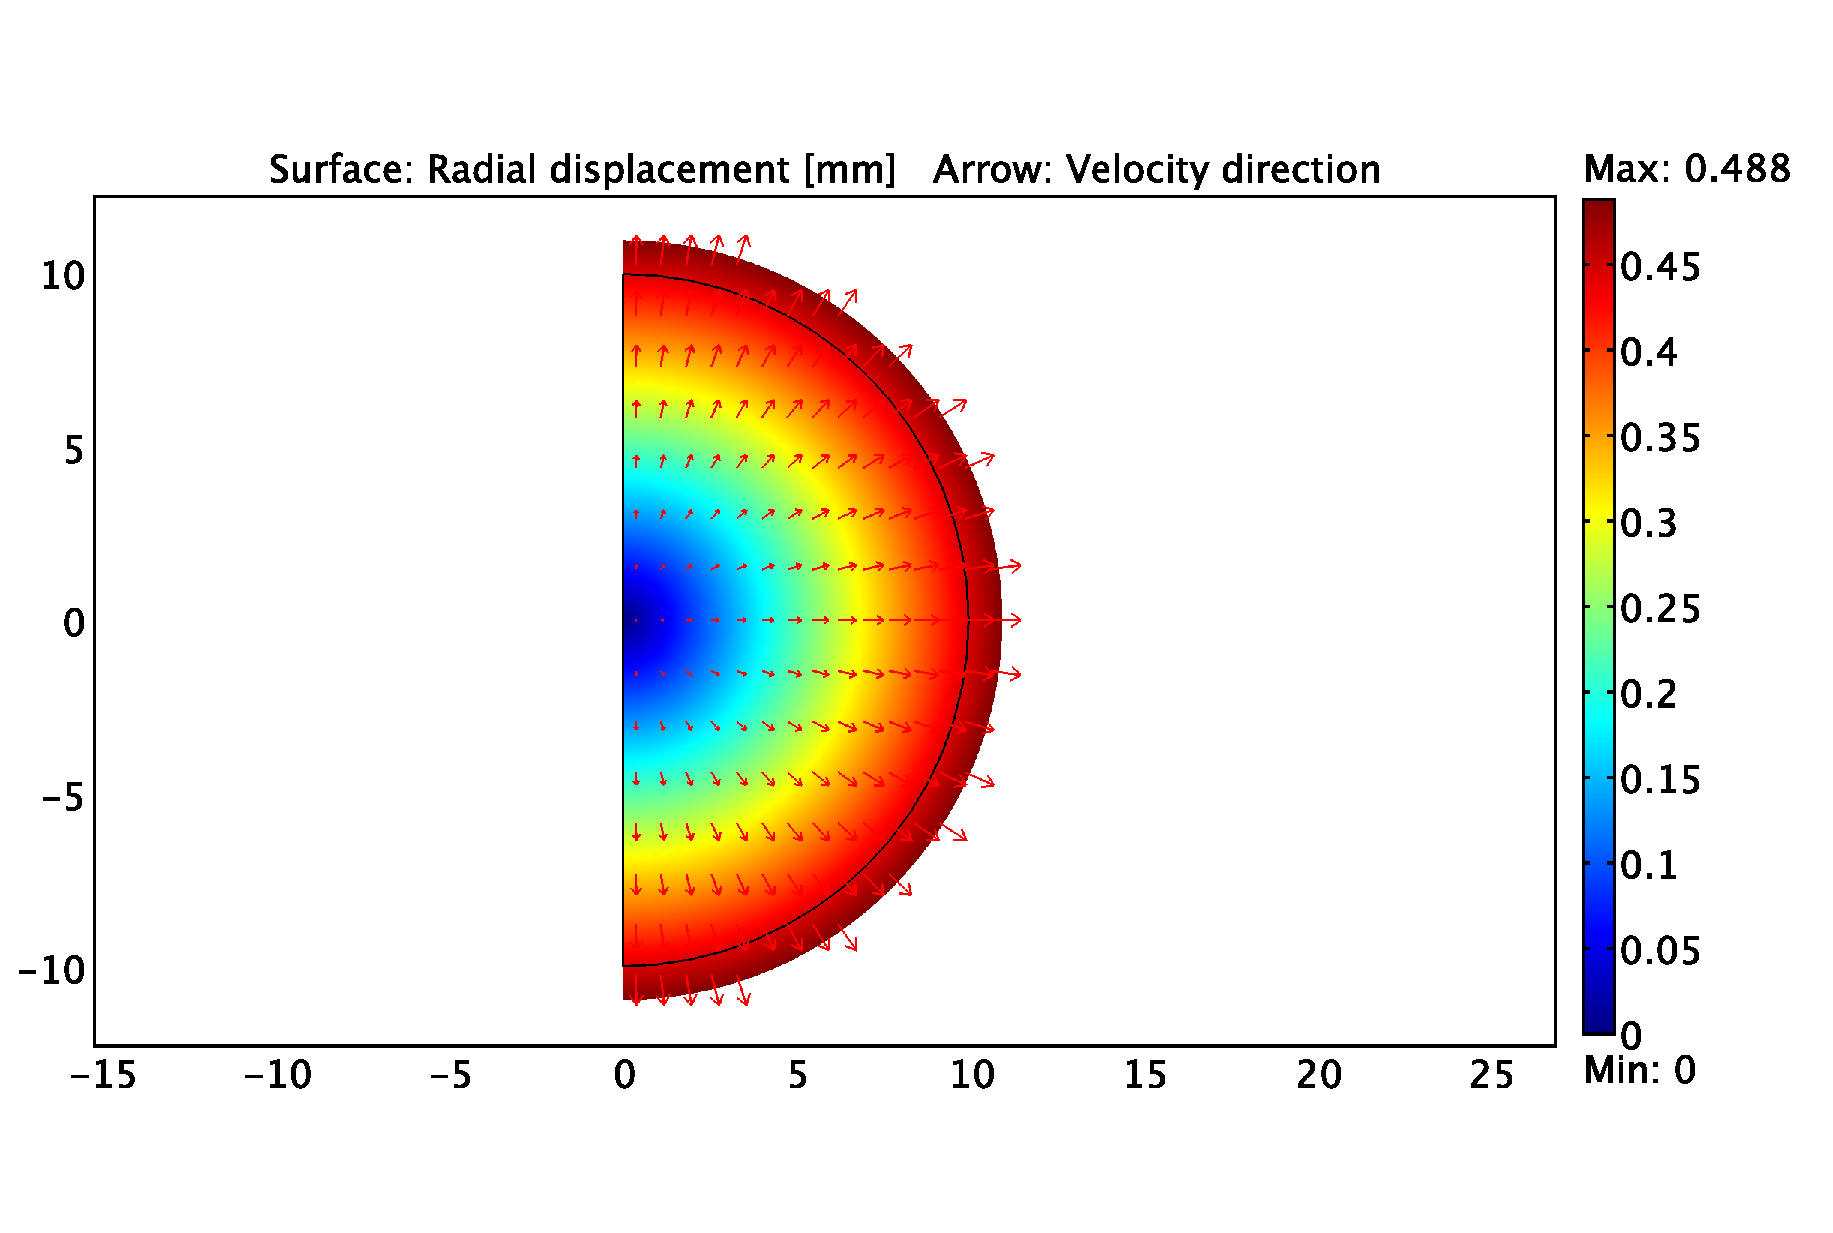
\includegraphics[width=0.8\textwidth]{images/examples/%
eulerian/cancer/isotropic-swelling-100}
\caption{A semicircular tumour at time $t=100$ days.}
\label{tumour-isotropic-swelling-100}
\end{figure}

\begin{figure}[!hptb]
\centering
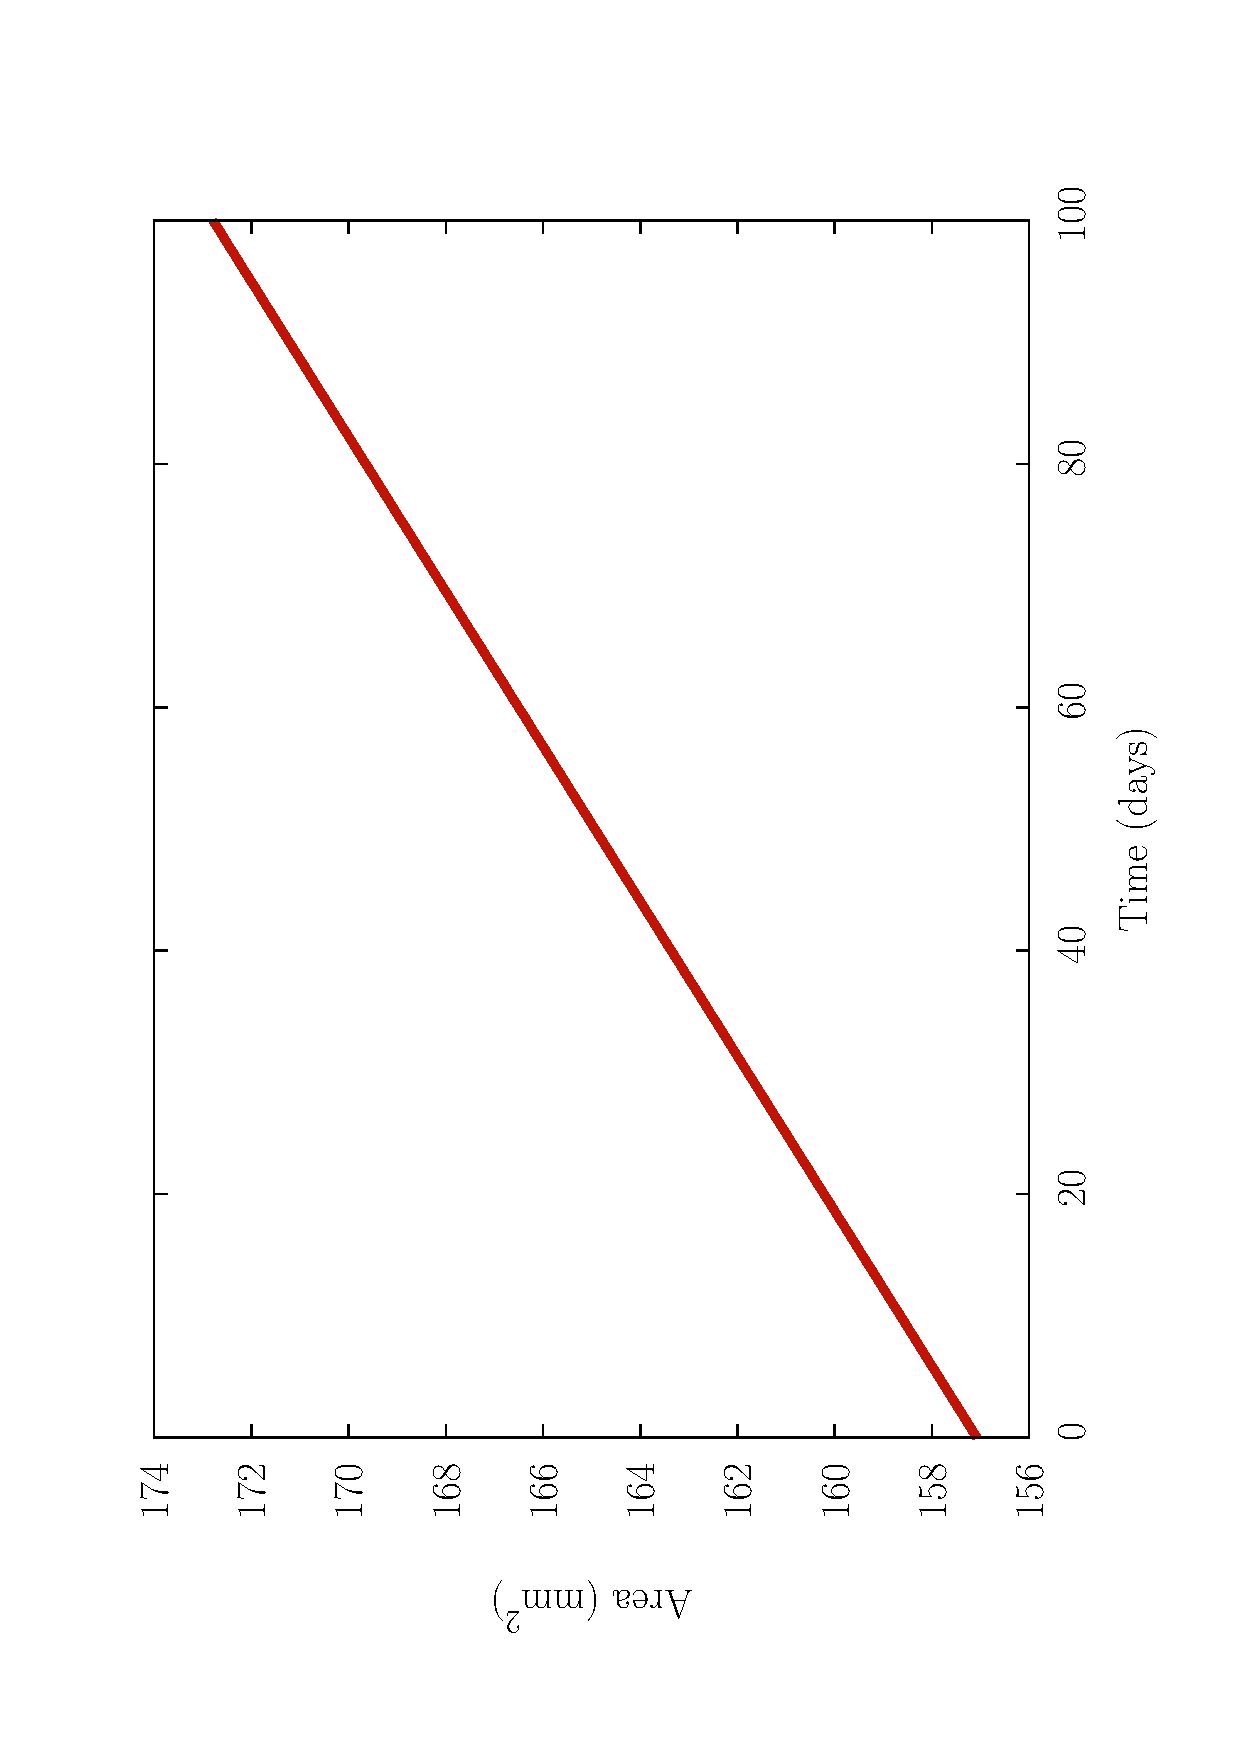
\includegraphics[width=0.6\textwidth,angle=270]{images/examples/%
eulerian/cancer/isotropic-swelling-area-evolution}
\caption{The area of the tumour evolving over 100 days.}
\label{tumour-isotropic-area-evolution}
\end{figure}

\subsection{Constrained by a wall}
\label{wall-constraint}

\begin{figure}[!hptb]
\centering
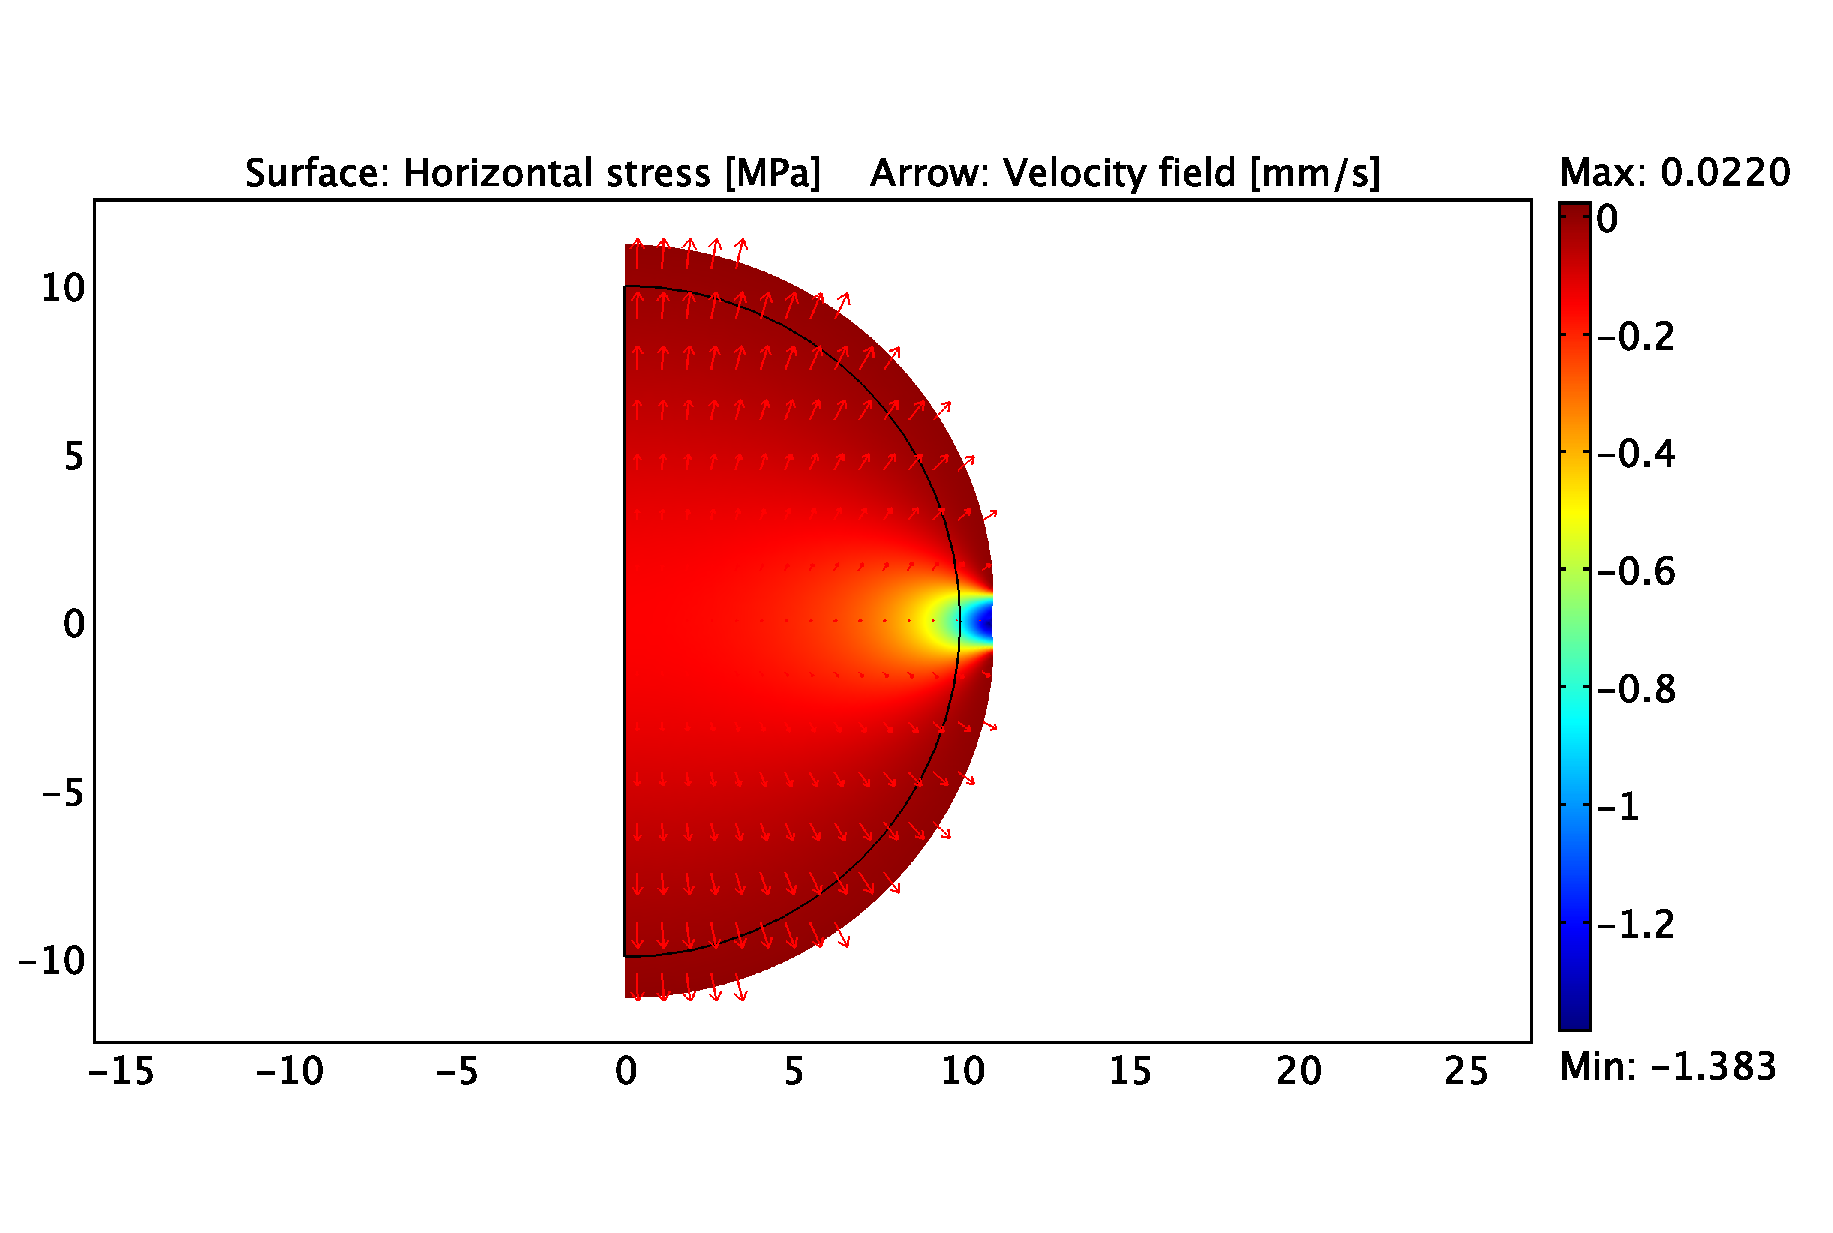
\includegraphics[width=0.8\textwidth]{images/examples/%
eulerian/cancer/constrained-swelling-120}
\caption{The growing tumour constrained by a wall at time $t=100$ days.}
\label{tumour-constrained-swelling-120}
\end{figure}

\begin{figure}[!hptb]
\centering
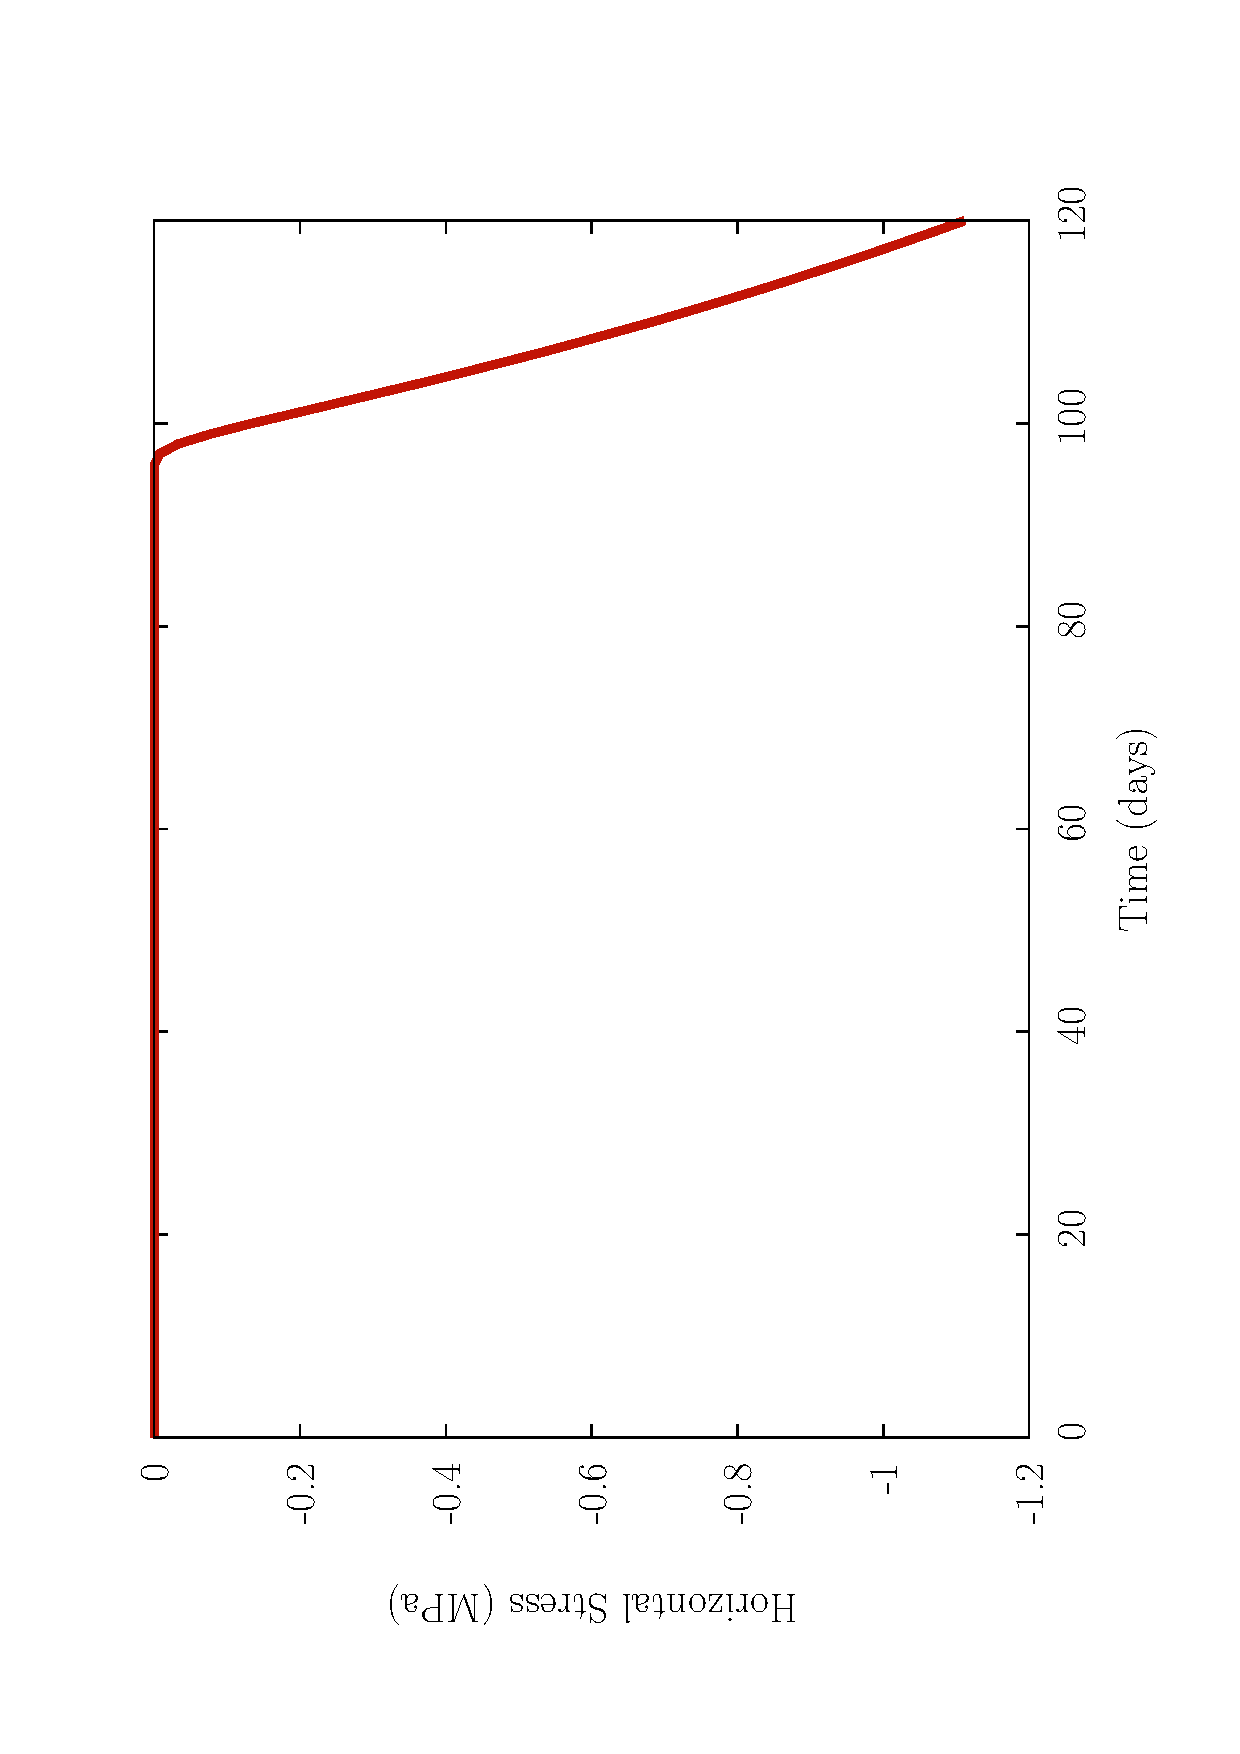
\includegraphics[width=0.6\textwidth,angle=270]{images/examples/%
eulerian/cancer/constrained-stress-evolution}
\caption{The horizontal stress in the tumour evolving over 120 days.}
\label{tumour-constrained-stress-evolution}
\end{figure}

\subsection{The role of the cells}
\label{cell-roles}

\subsubsection{Inward tug}
\label{inward-tug}

\begin{figure}[!hptb]
\centering
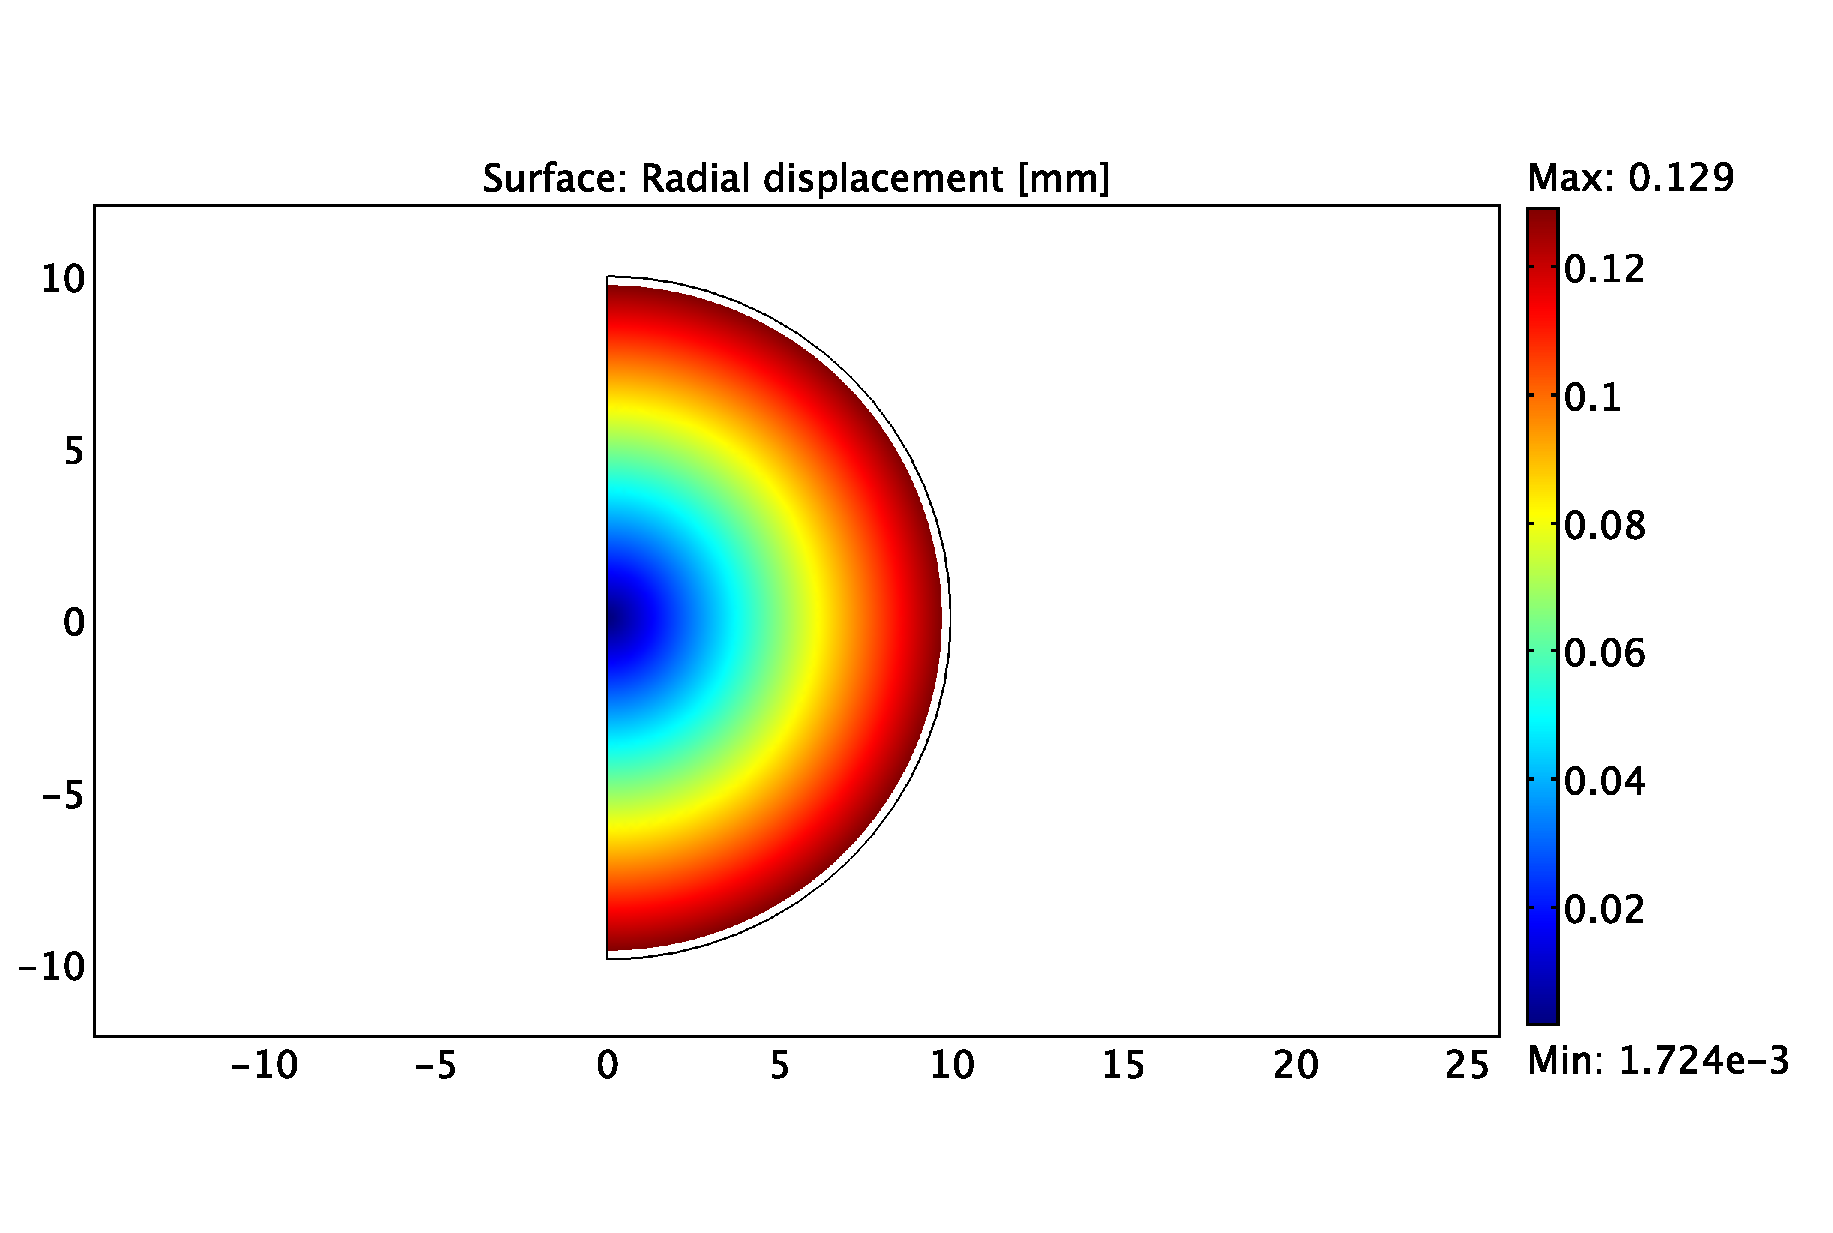
\includegraphics[width=0.8\textwidth]{images/examples/%
eulerian/cancer/homogeneous-inward-tug}
\caption{Homogeneous inward tug due to a uniform distribution of cells.}
\label{tumour-homogeneous-inward-tug}
\end{figure}

\begin{figure}[!hptb]
\centering
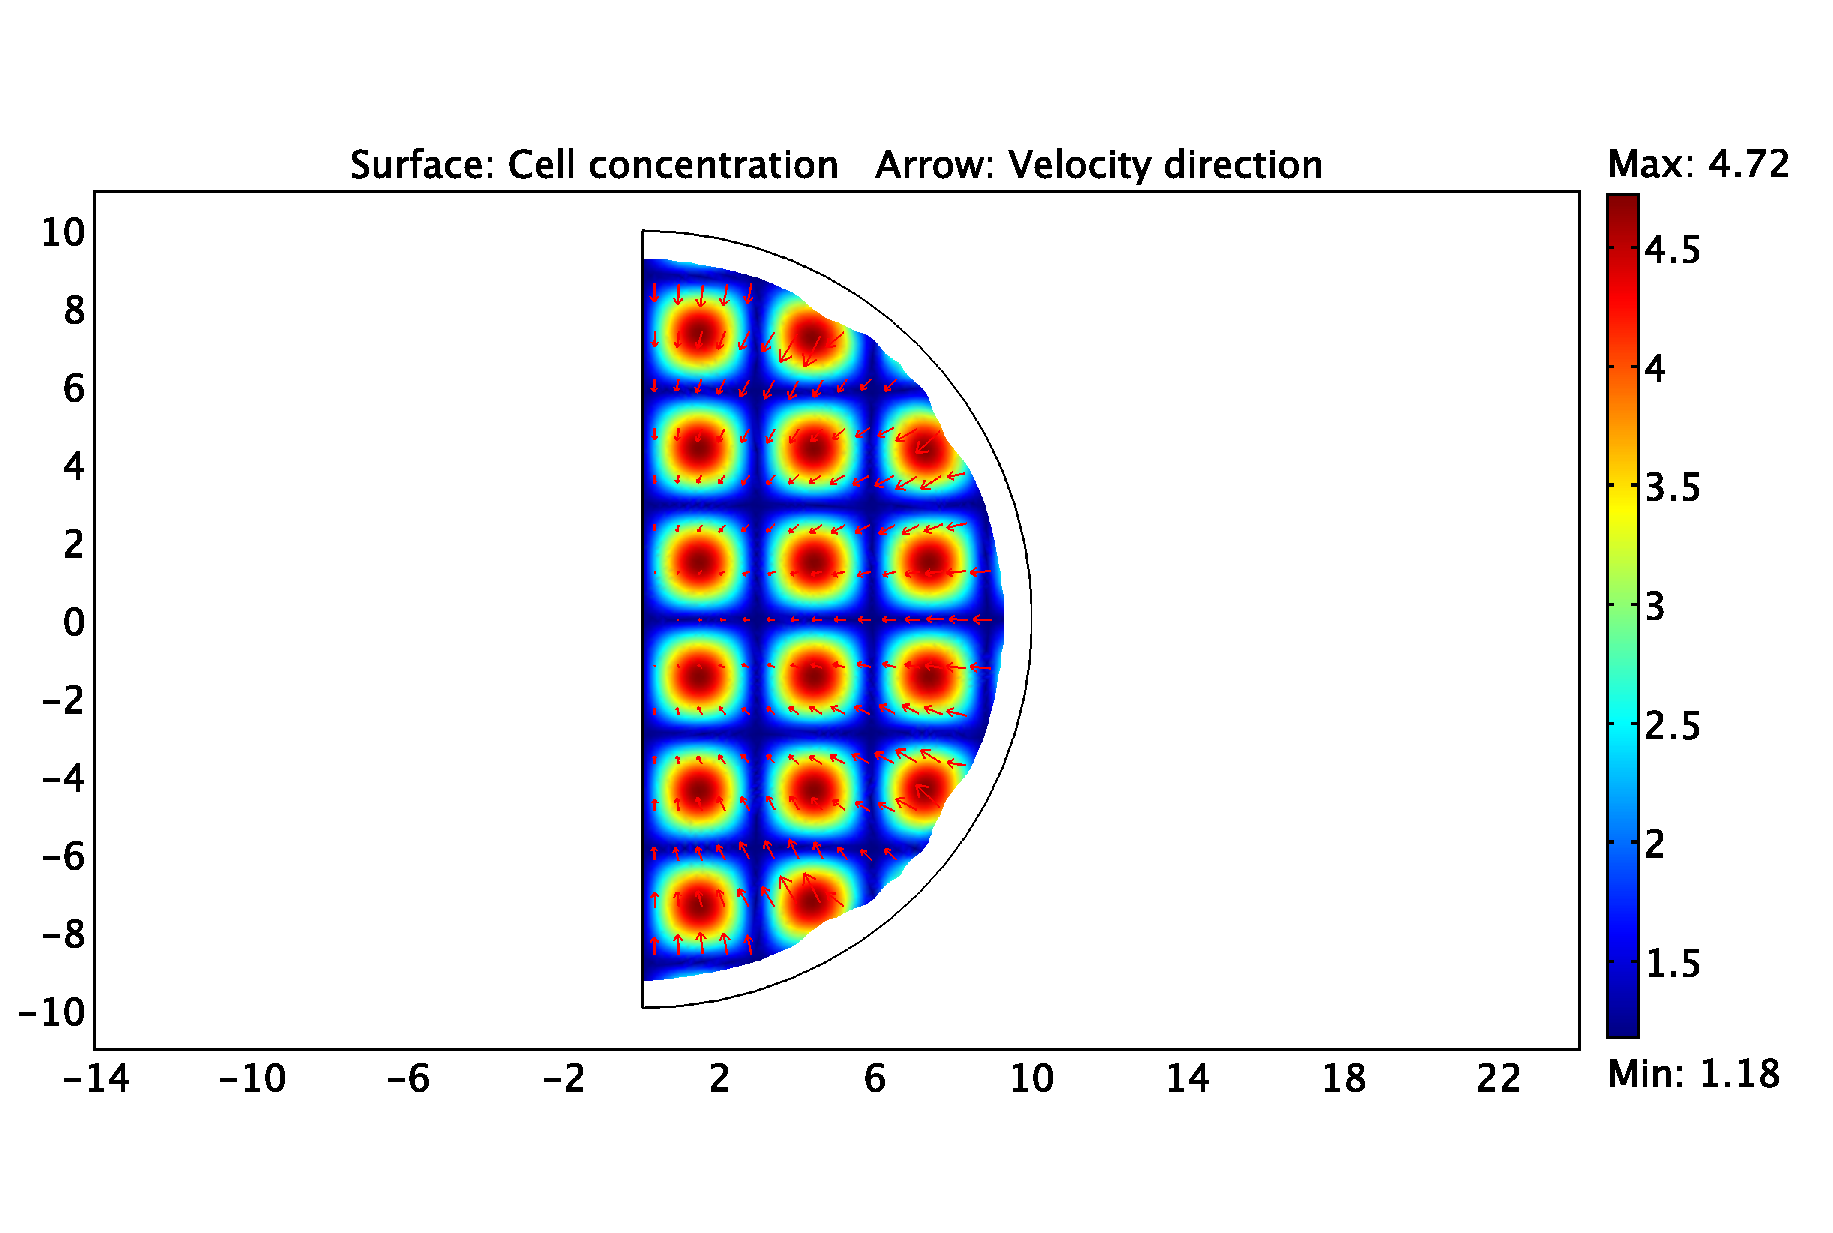
\includegraphics[width=0.8\textwidth]{images/examples/%
eulerian/cancer/heterogeneous-inward-tug}
\caption{Heterogeneous inward tug due to a non-uniform distribution of cells.}
\label{tumour-heterogeneous-inward-tug}
\end{figure}

\subsubsection{Transport of the cells}
\label{cell-transport}

{\bf Diffusion and proliferation}

\begin{figure}[!hptb]
\centering
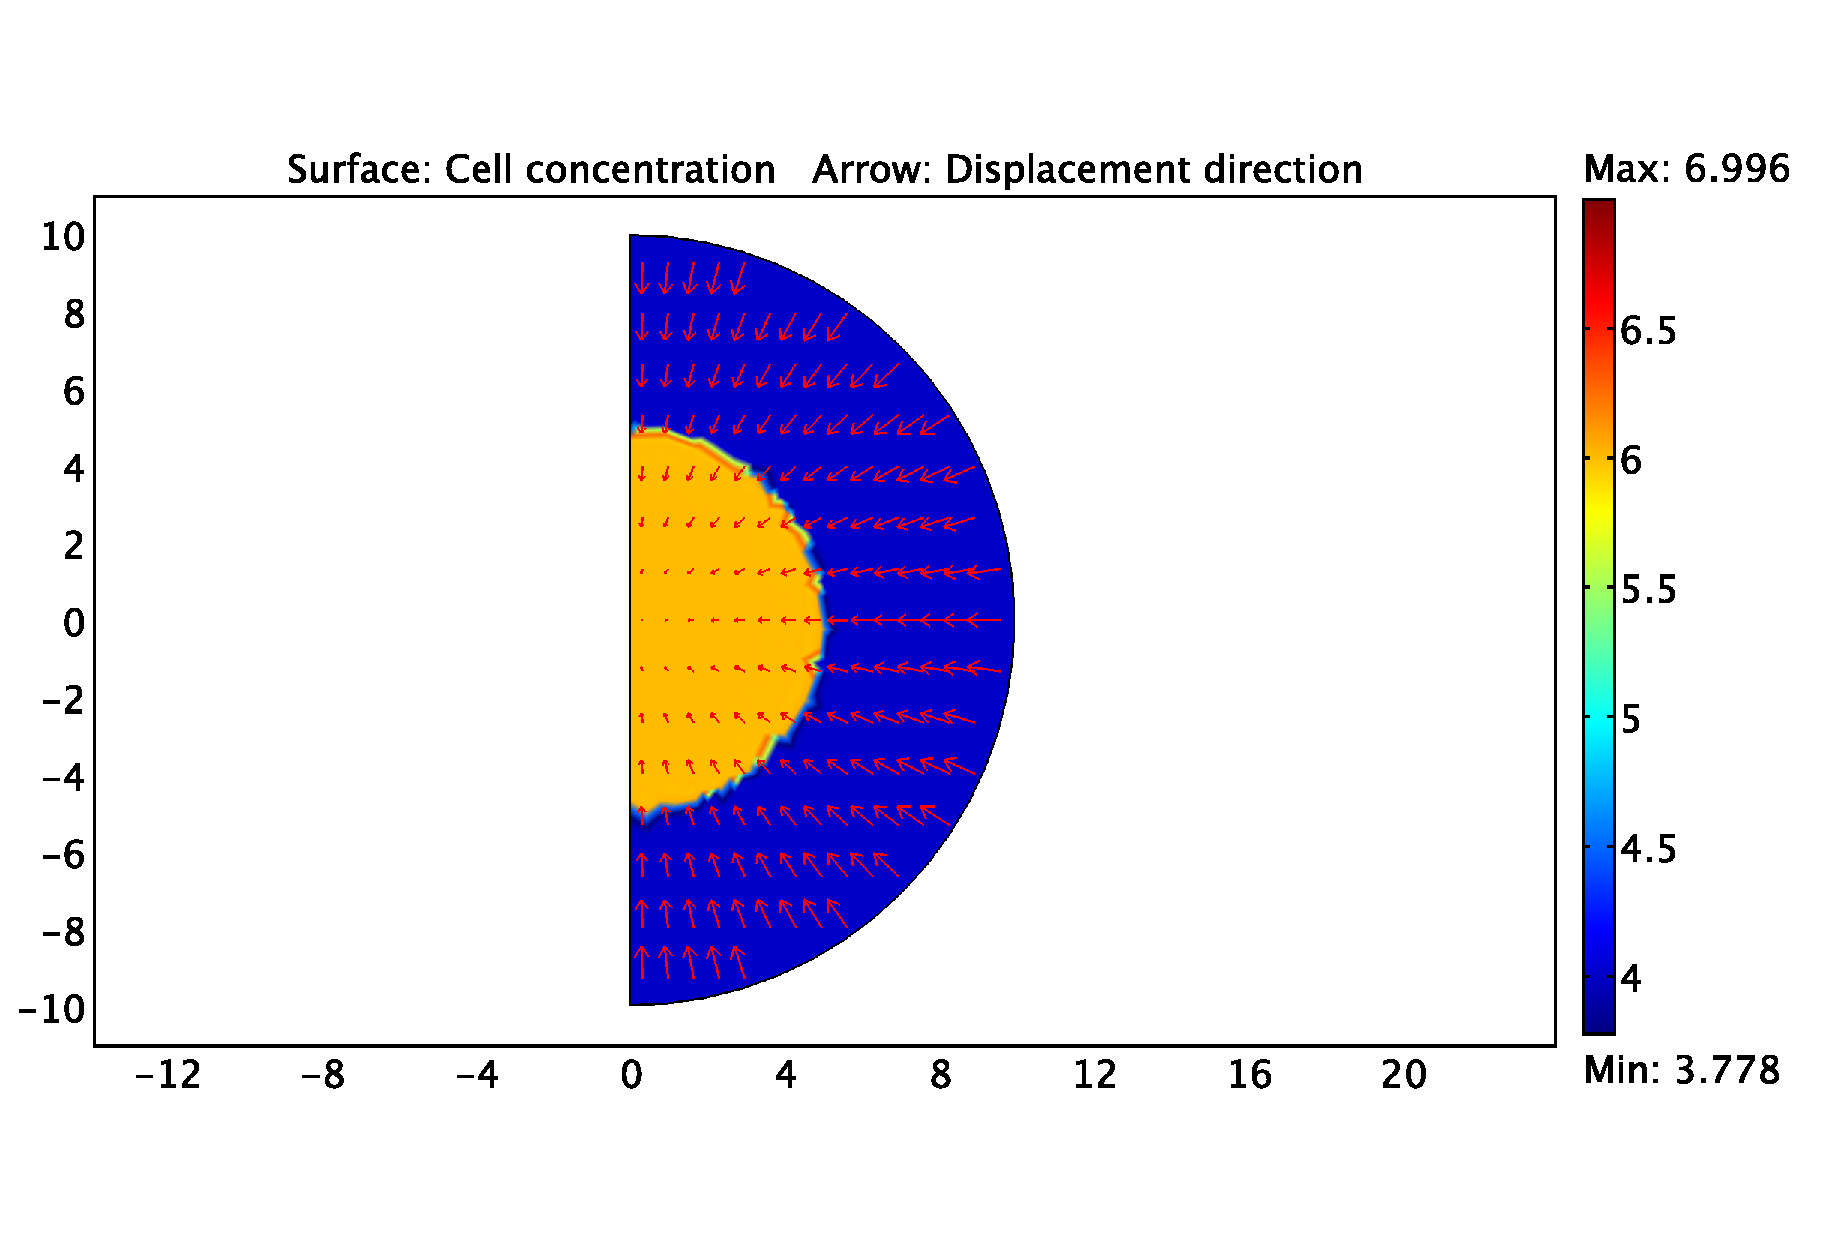
\includegraphics[width=0.8\textwidth]{images/examples/%
eulerian/cancer/diffusing-proliferating-cells-0}
\caption{The cells diffusing and proliferating at time $t=0$ days.}
\label{tumour-diffusion-proliferation-0}
\end{figure}

\begin{figure}[!hptb]
\centering
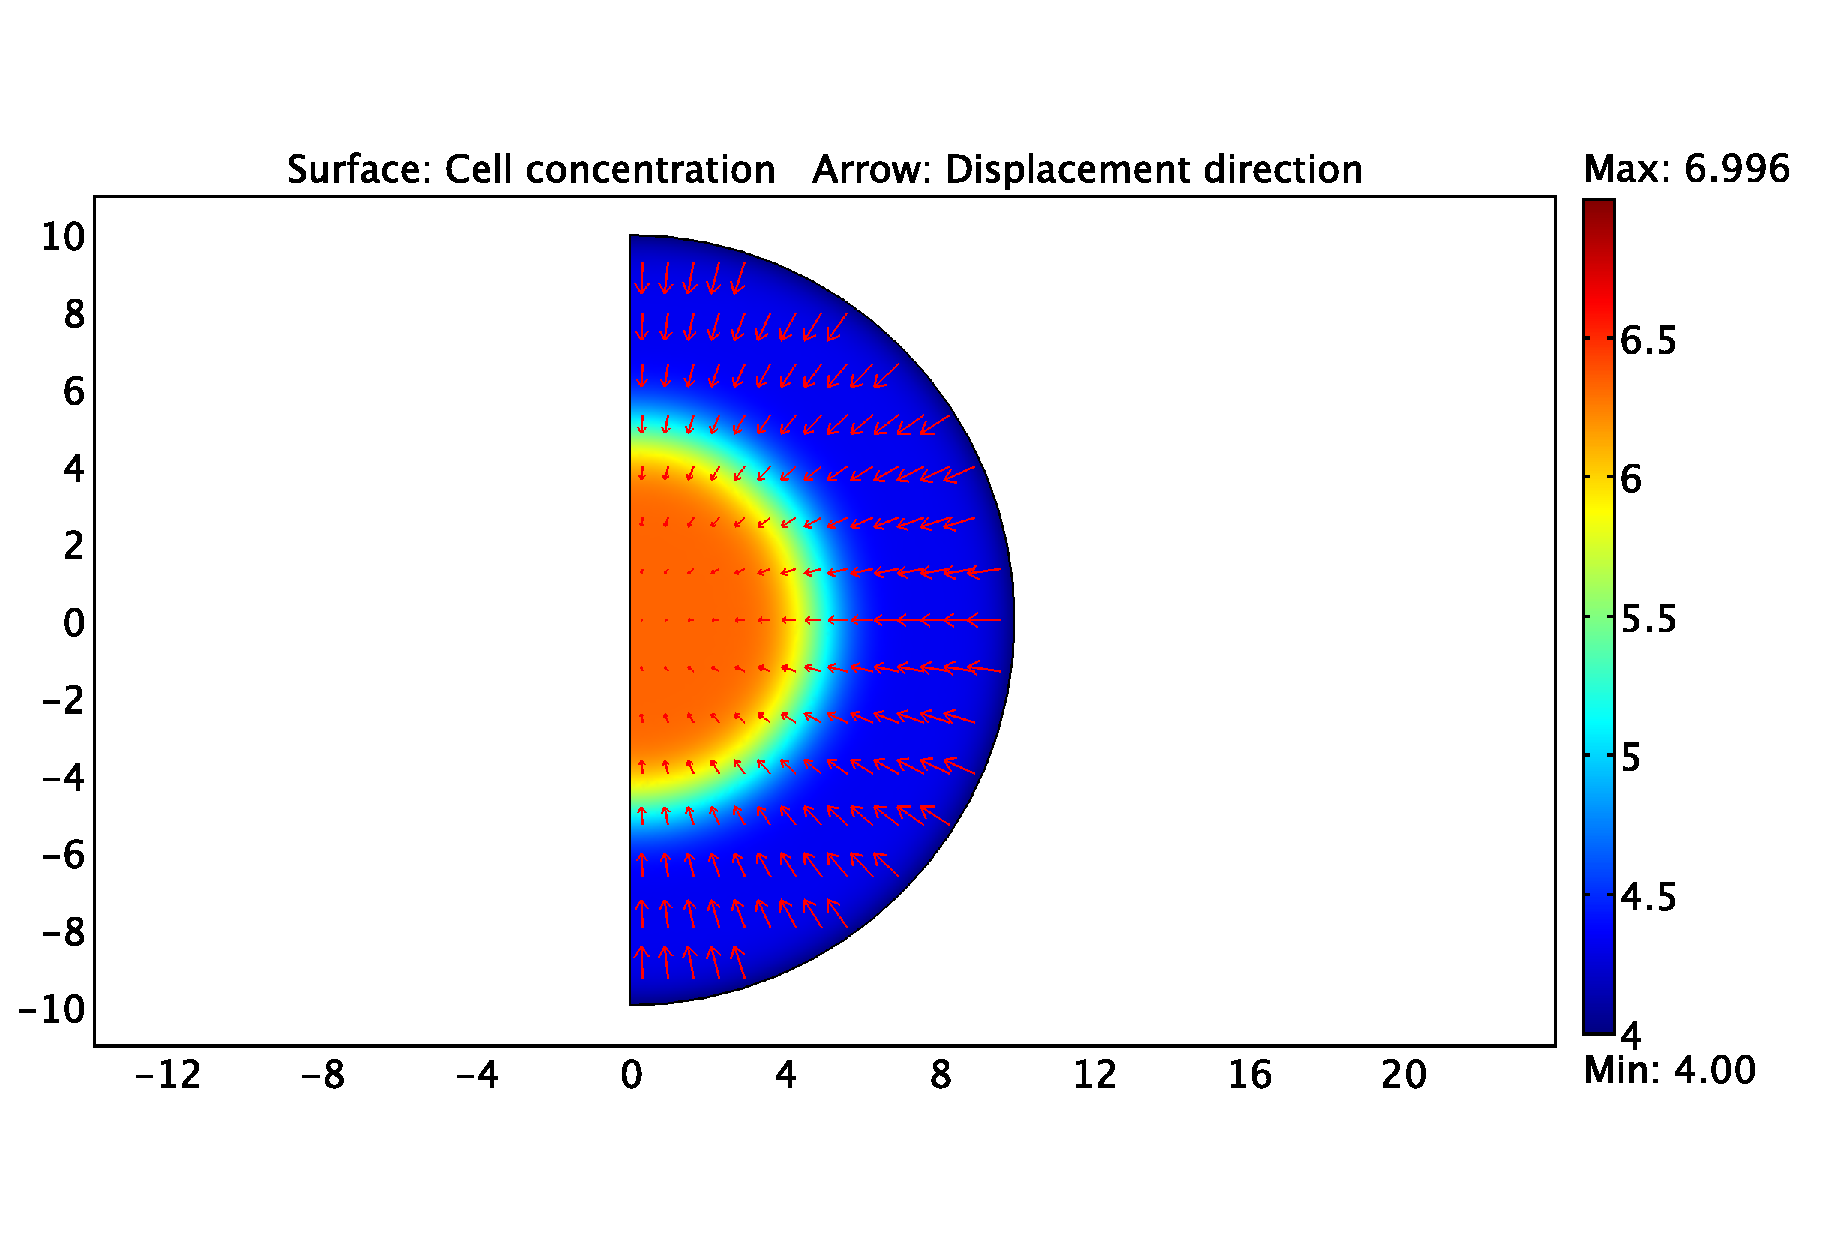
\includegraphics[width=0.8\textwidth]{images/examples/%
eulerian/cancer/diffusing-proliferating-cells-33}
\caption{The cells diffusing and proliferating at time $t=33$ days.}
\label{tumour-diffusion-proliferation-33}
\end{figure}

\begin{figure}[!hptb]
\centering
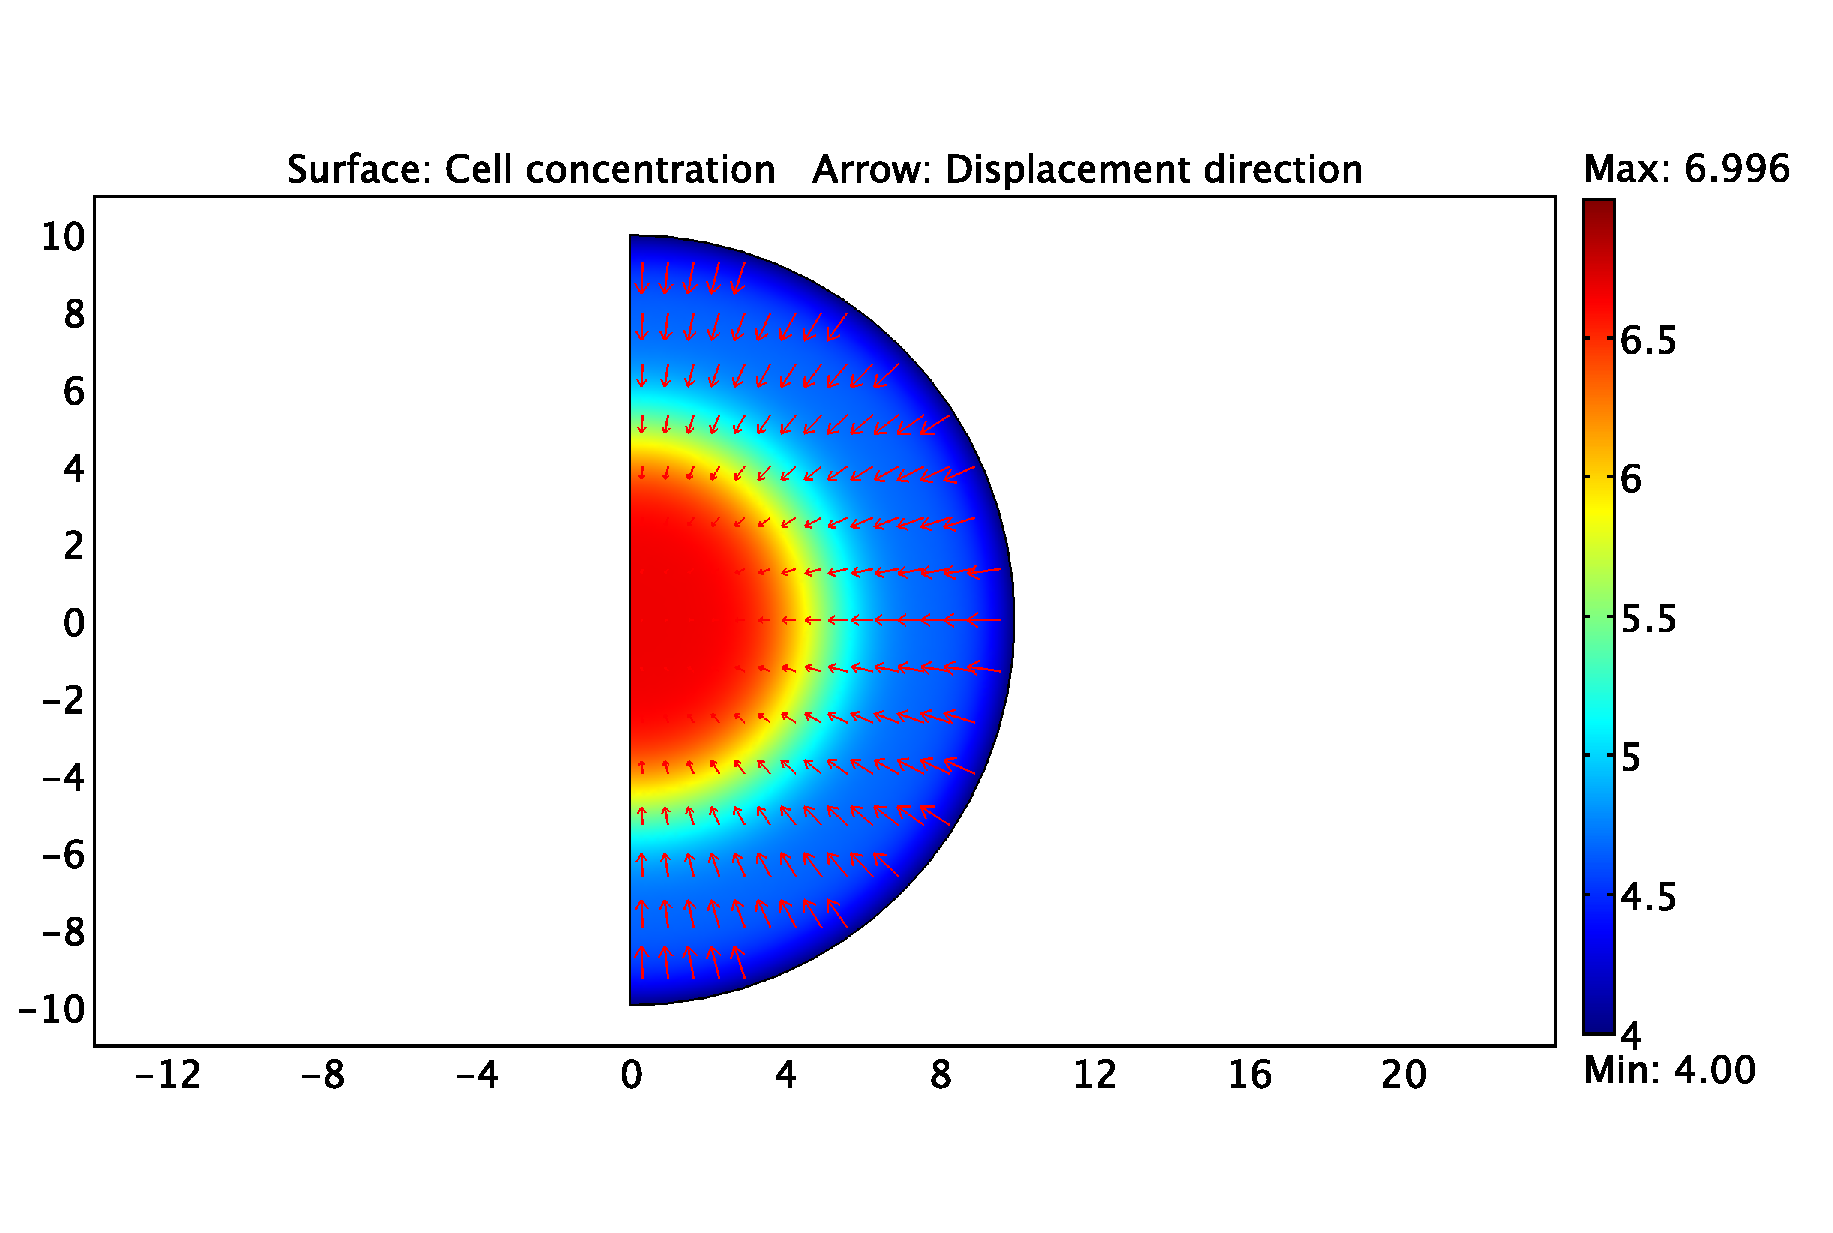
\includegraphics[width=0.8\textwidth]{images/examples/%
eulerian/cancer/diffusing-proliferating-cells-67}
\caption{The cells diffusing and proliferating at time $t=67$ days.}
\label{tumour-diffusion-proliferation-67}
\end{figure}

\begin{figure}[!hptb]
\centering
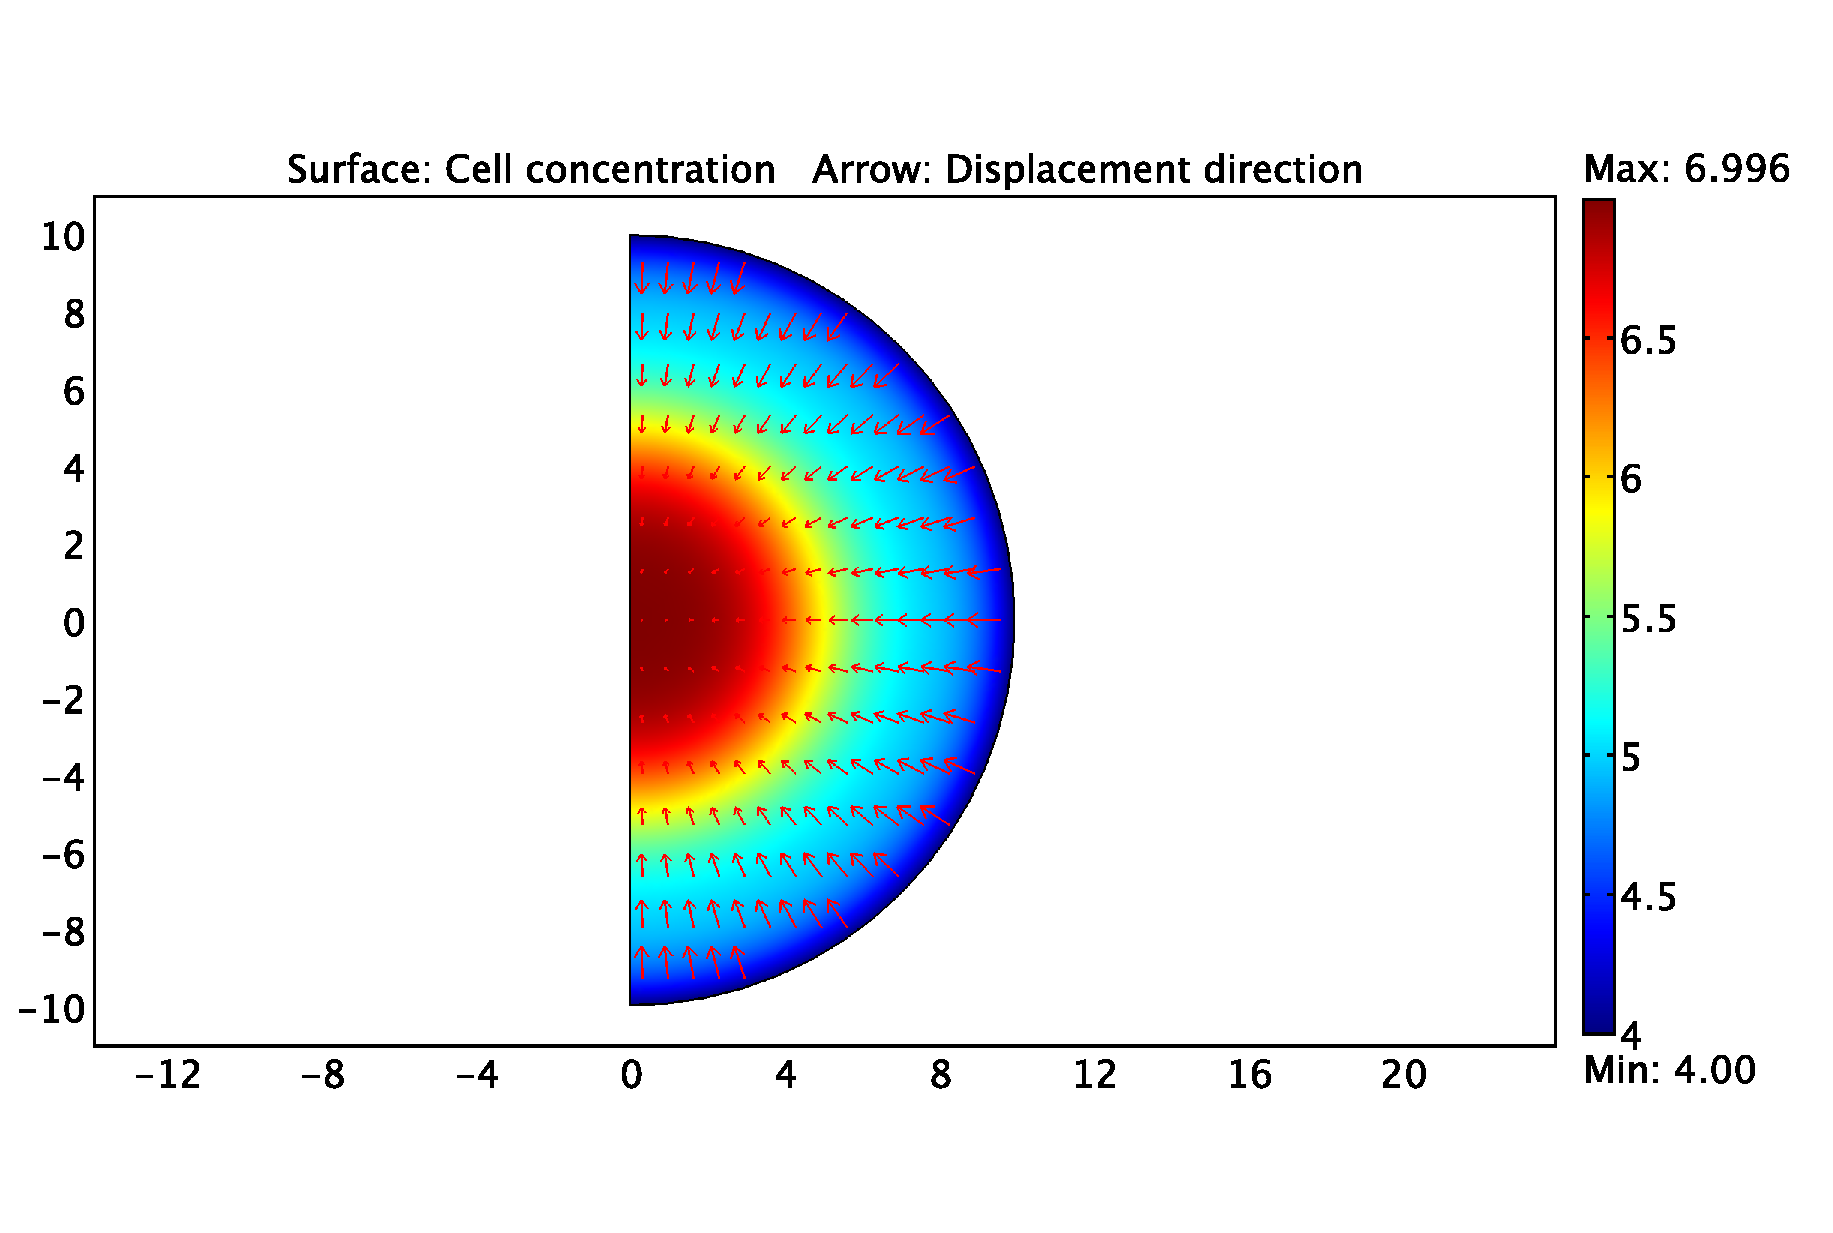
\includegraphics[width=0.8\textwidth]{images/examples/%
eulerian/cancer/diffusing-proliferating-cells-100}
\caption{The cells diffusing and proliferating at time $t=100$ days.}
\label{tumour-diffusion-proliferation-100}
\end{figure}

{\bf Haptotaxis}

\begin{figure}[!hptb]
\centering
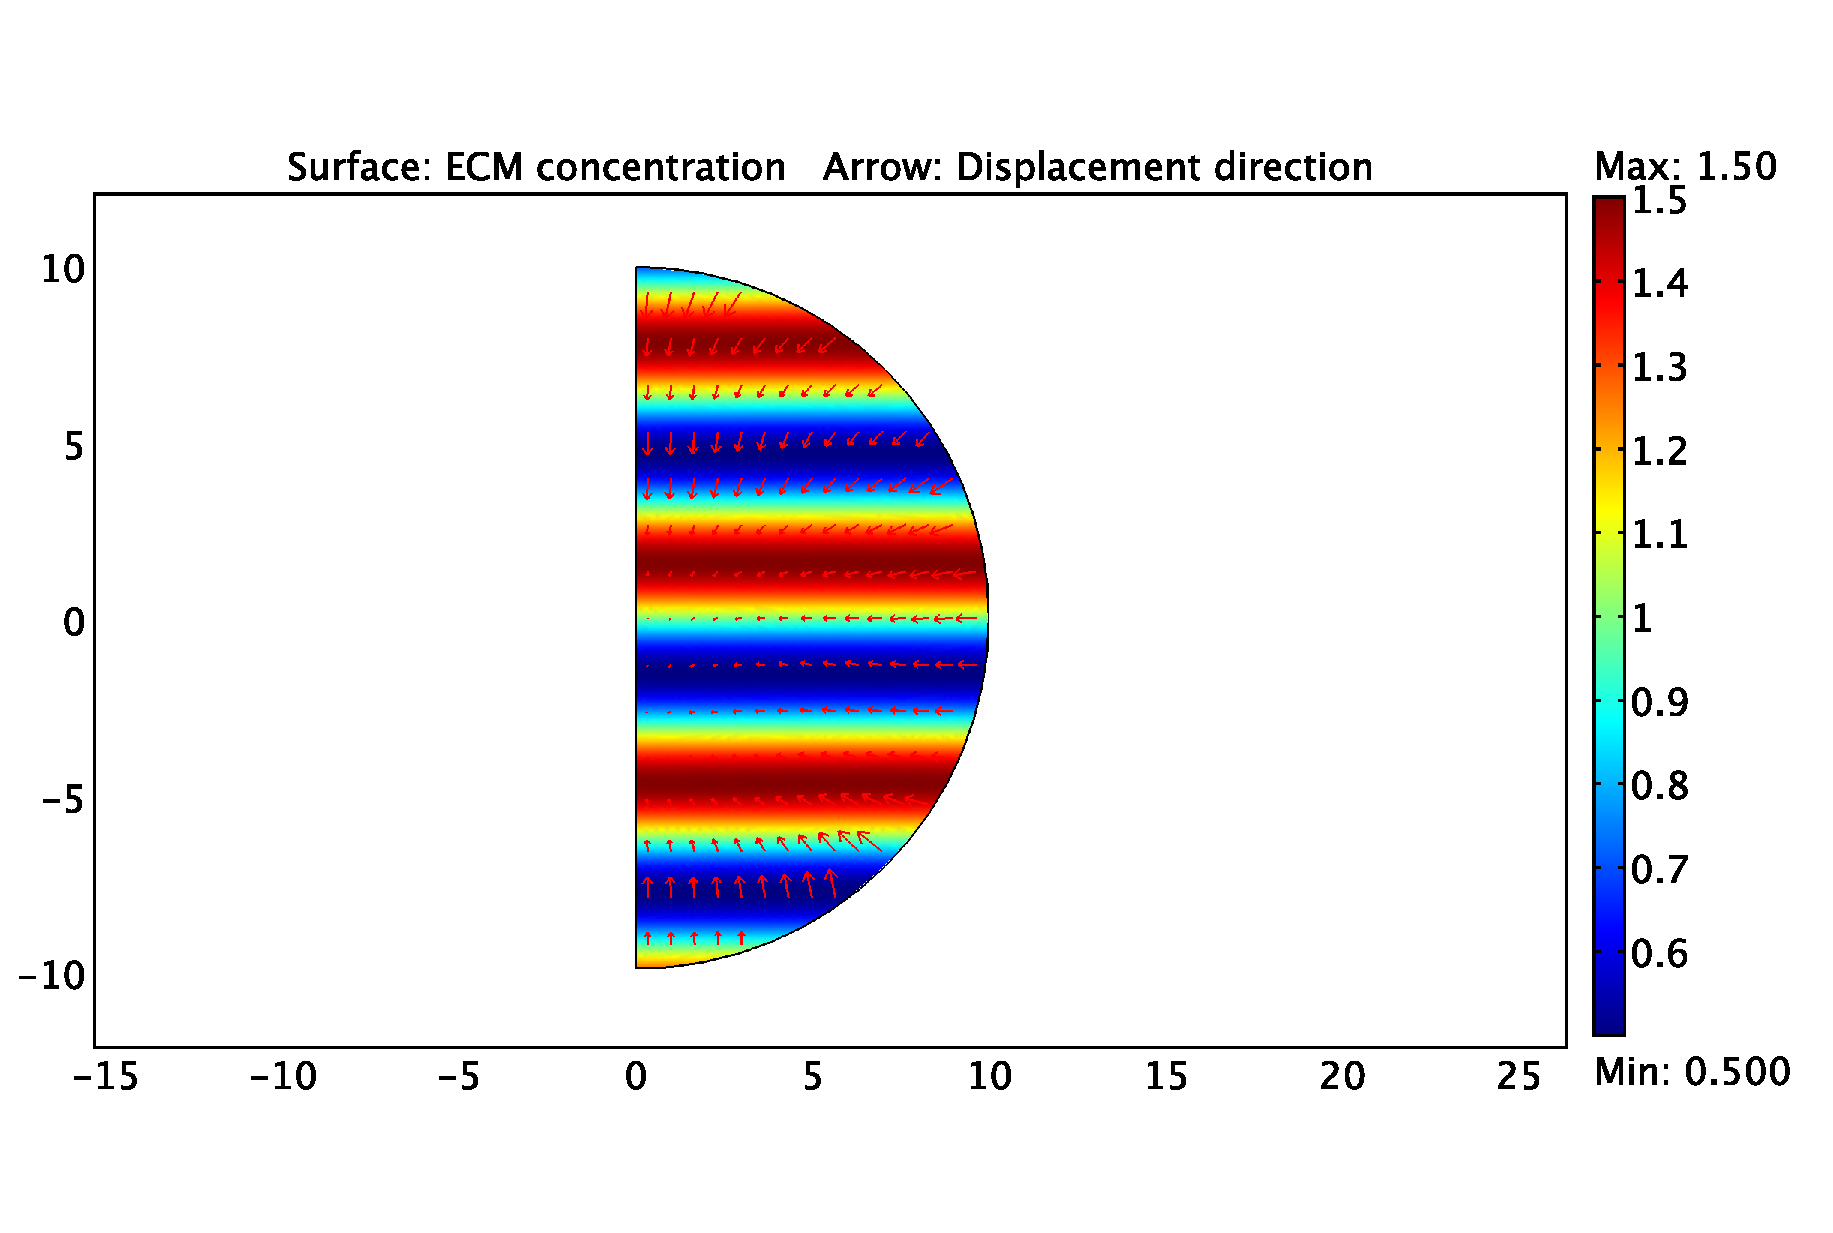
\includegraphics[width=0.8\textwidth]{images/examples/%
eulerian/cancer/heterogeneous-ecm-concentration}
\caption{Heterogeneous extra-cellular matrix concentration.}
\label{heterogeneous-ecm-concentration}
\end{figure}

\begin{figure}[!hptb]
\centering
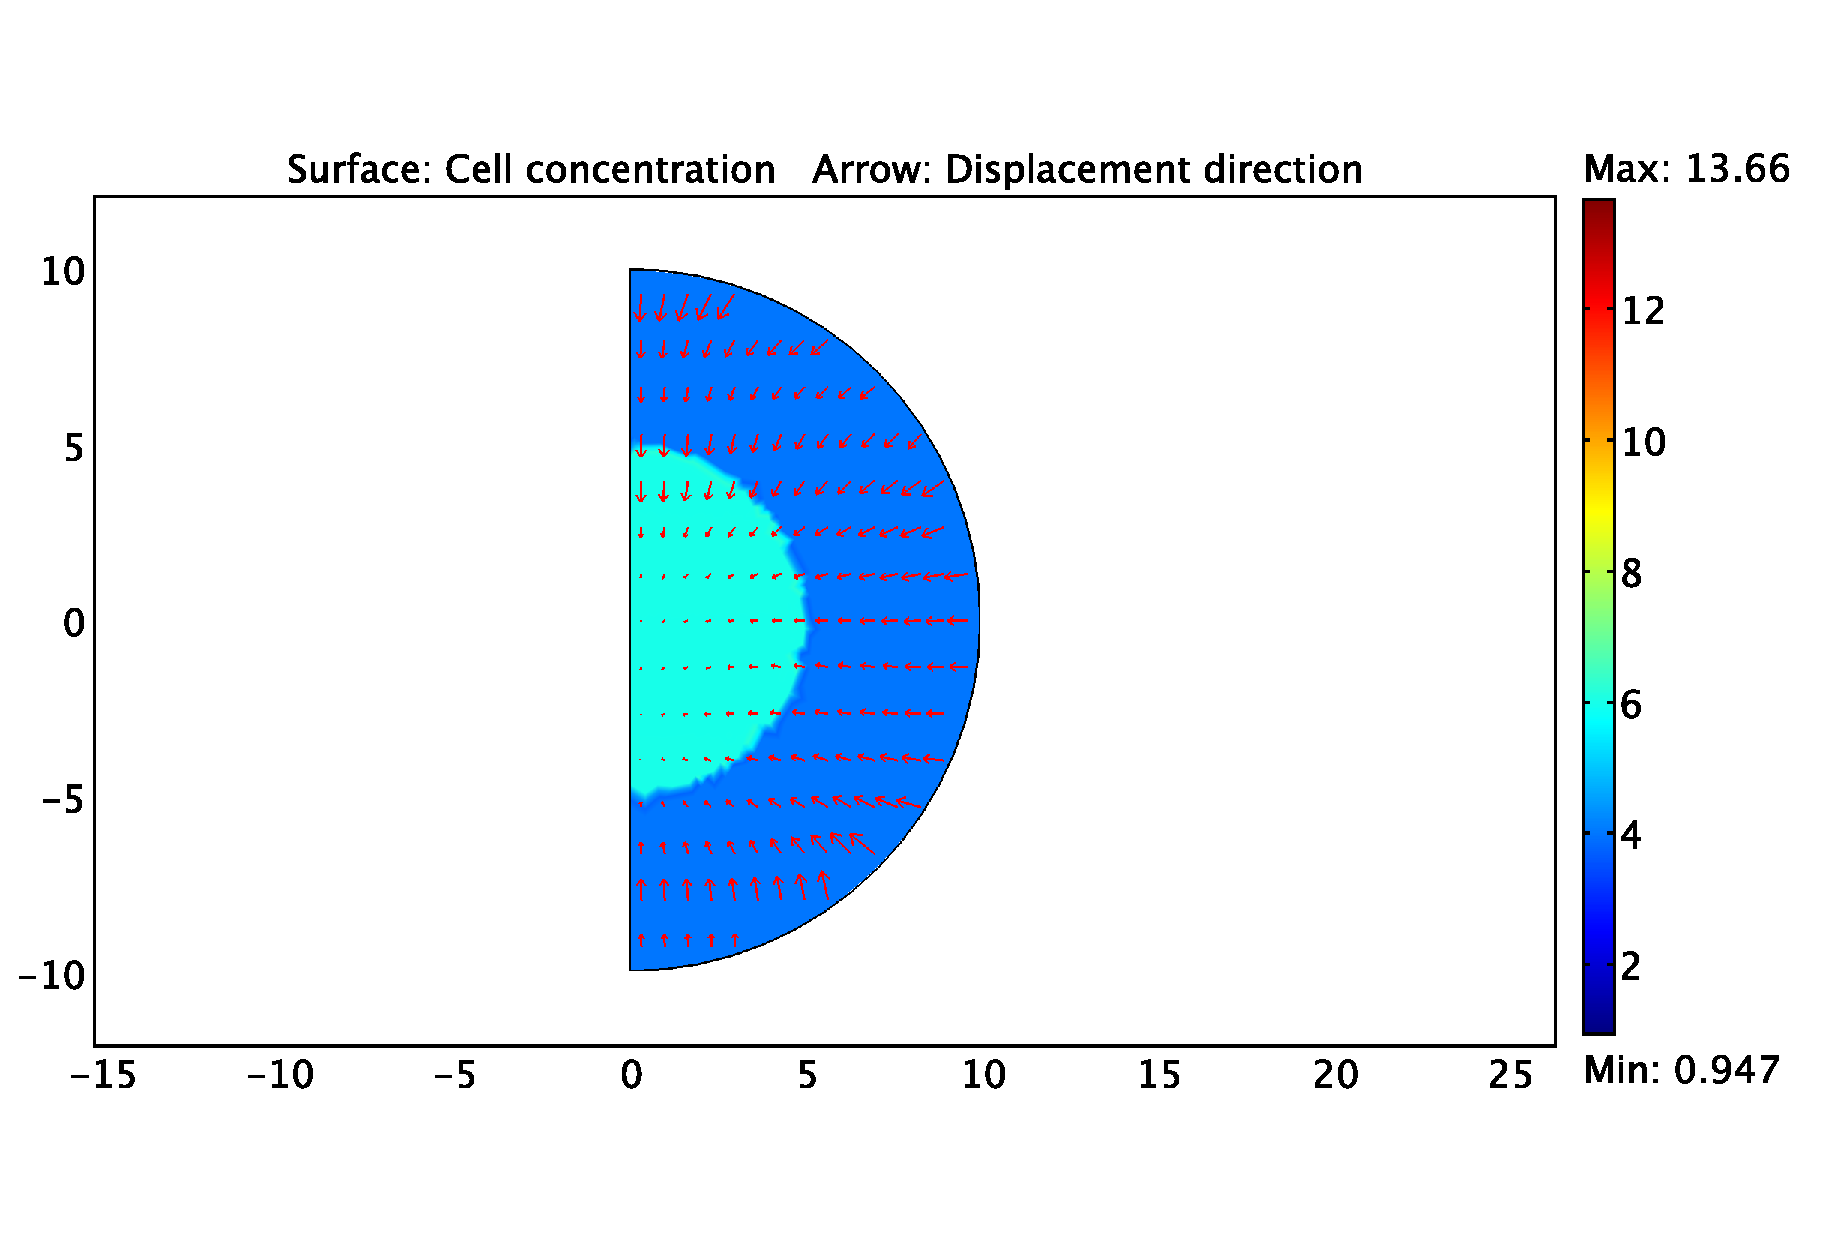
\includegraphics[width=0.8\textwidth]{images/examples/%
eulerian/cancer/haptotaxis-proliferating-cells-0}
\caption{Proliferating cells undergoing diffusion and haptotaxis at time $t=0$ days.}
\label{tumour-haptotaxis-proliferation-0}
\end{figure}

\begin{figure}[!hptb]
\centering
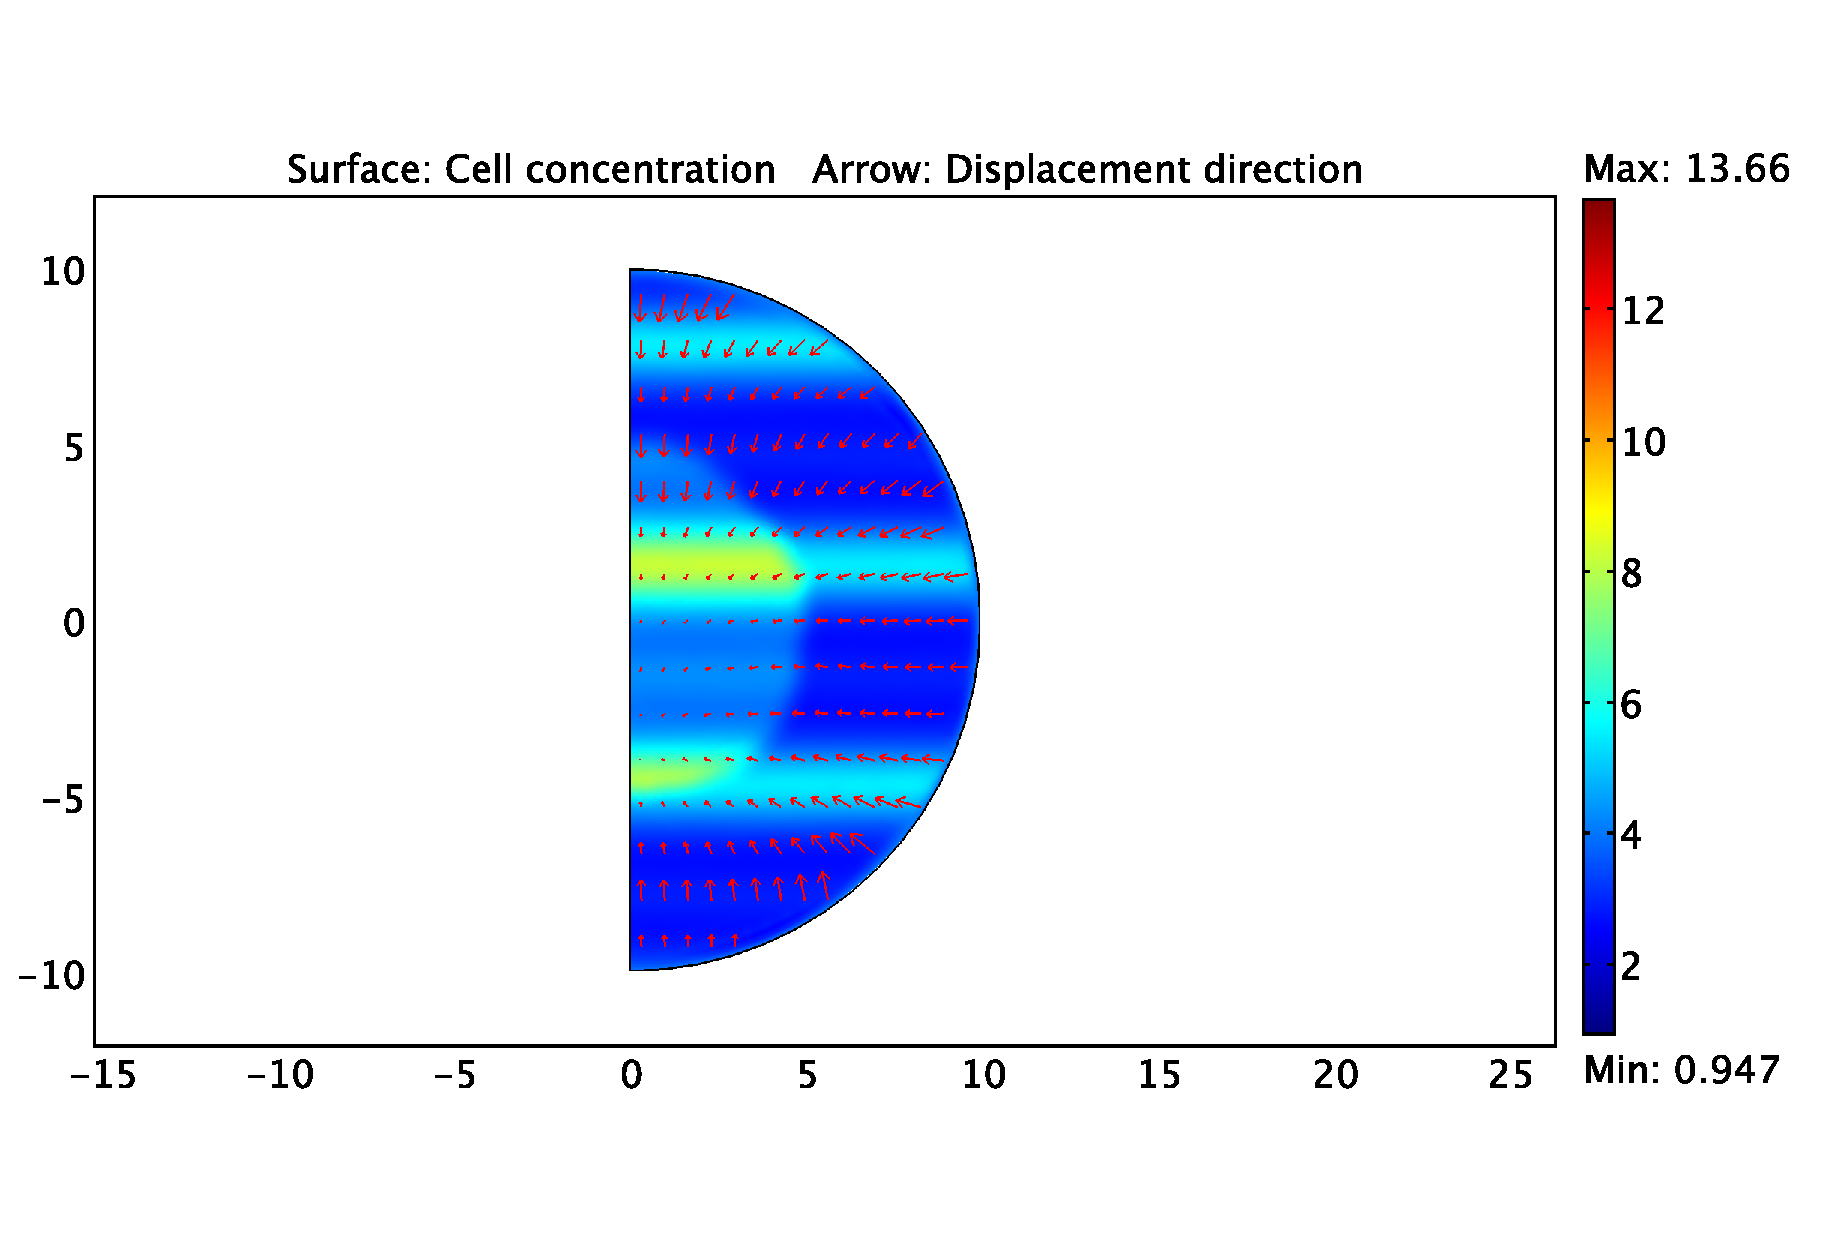
\includegraphics[width=0.8\textwidth]{images/examples/%
eulerian/cancer/haptotaxis-proliferating-cells-3p3}
\caption{Proliferating cells undergoing diffusion and haptotaxis at time $t=3.3$ days.}
\label{tumour-haptotaxis-proliferation-3p3}
\end{figure}

\begin{figure}[!hptb]
\centering
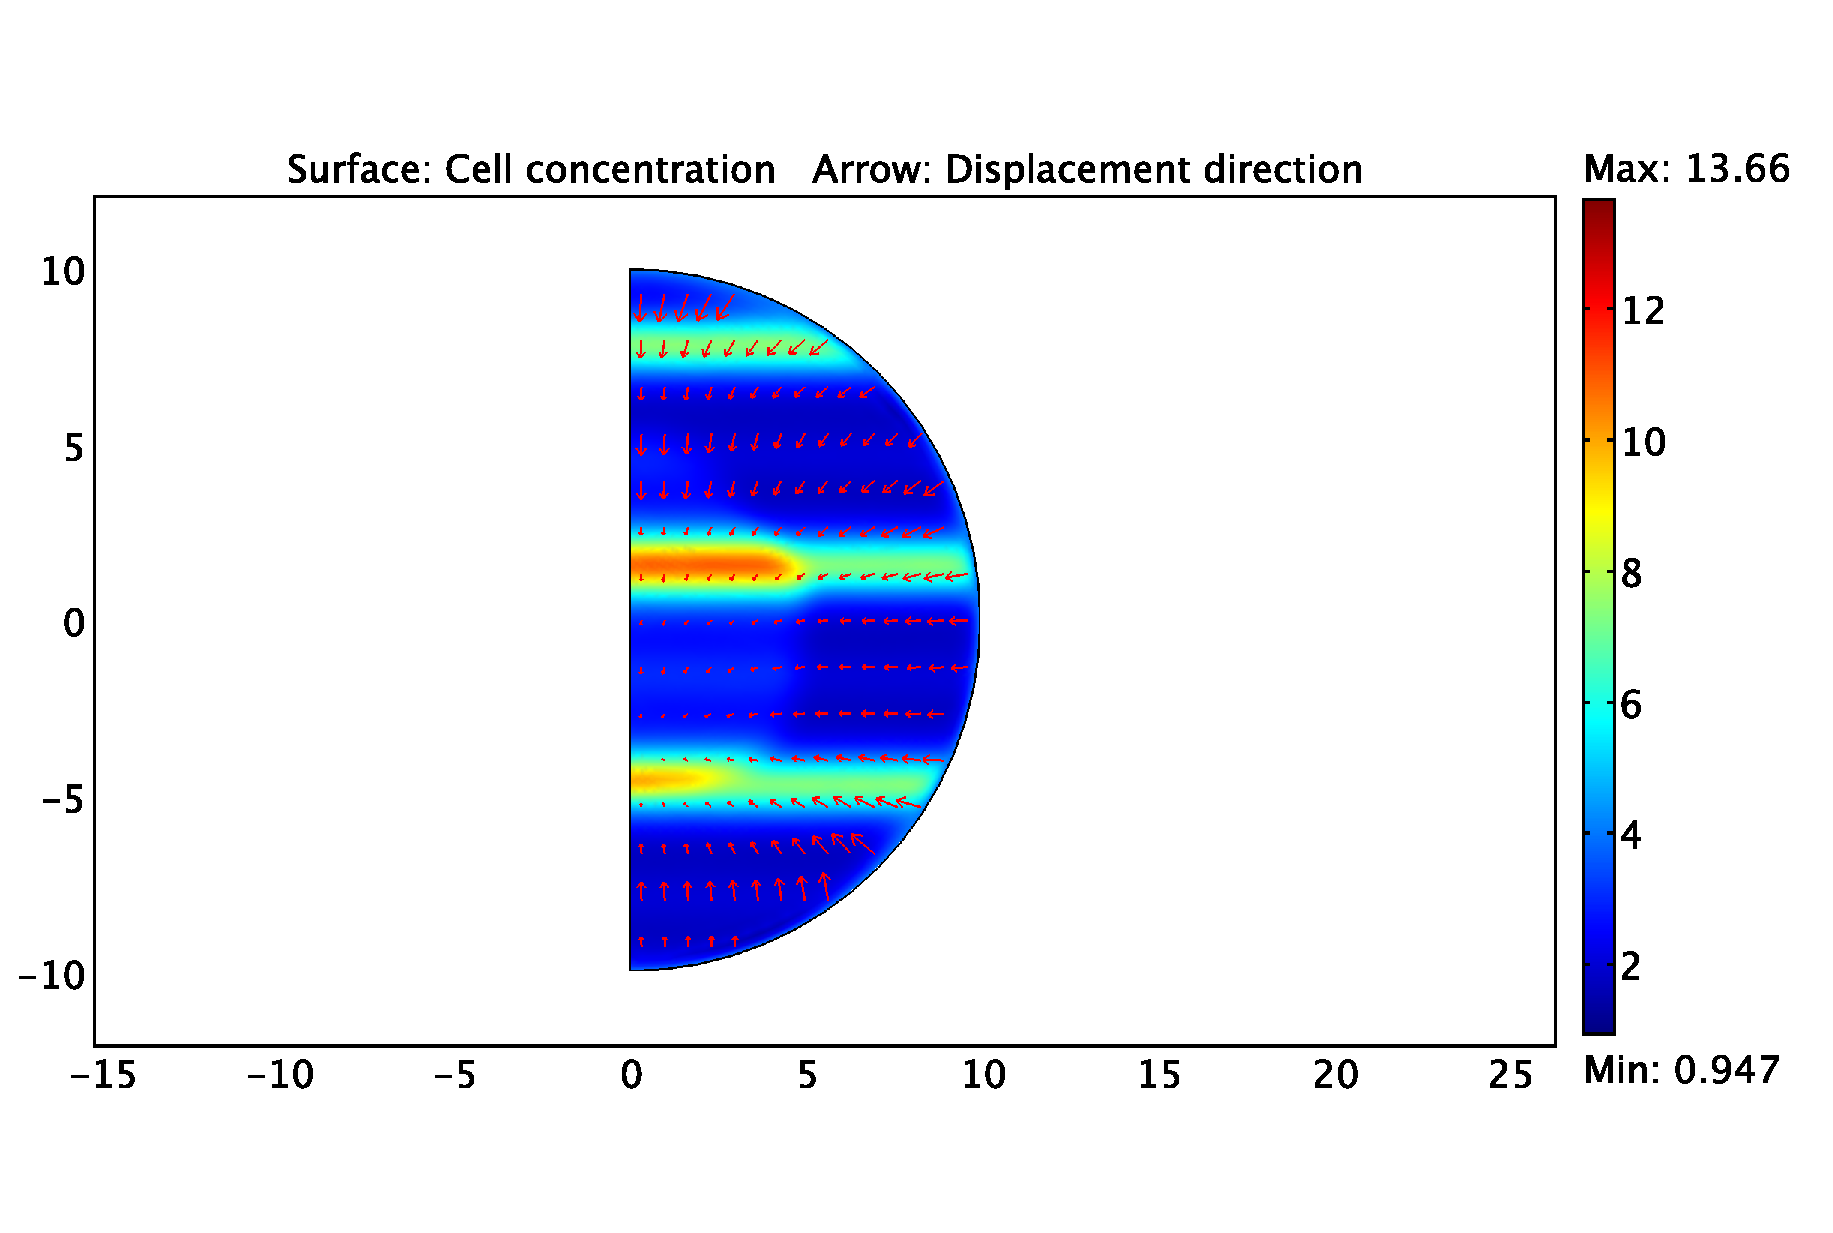
\includegraphics[width=0.8\textwidth]{images/examples/%
eulerian/cancer/haptotaxis-proliferating-cells-6p7}
\caption{Proliferating cells undergoing diffusion and haptotaxis at time $t=6.7$ days.}
\label{tumour-haptotaxis-proliferation-6p7}
\end{figure}

\begin{figure}[!hptb]
\centering
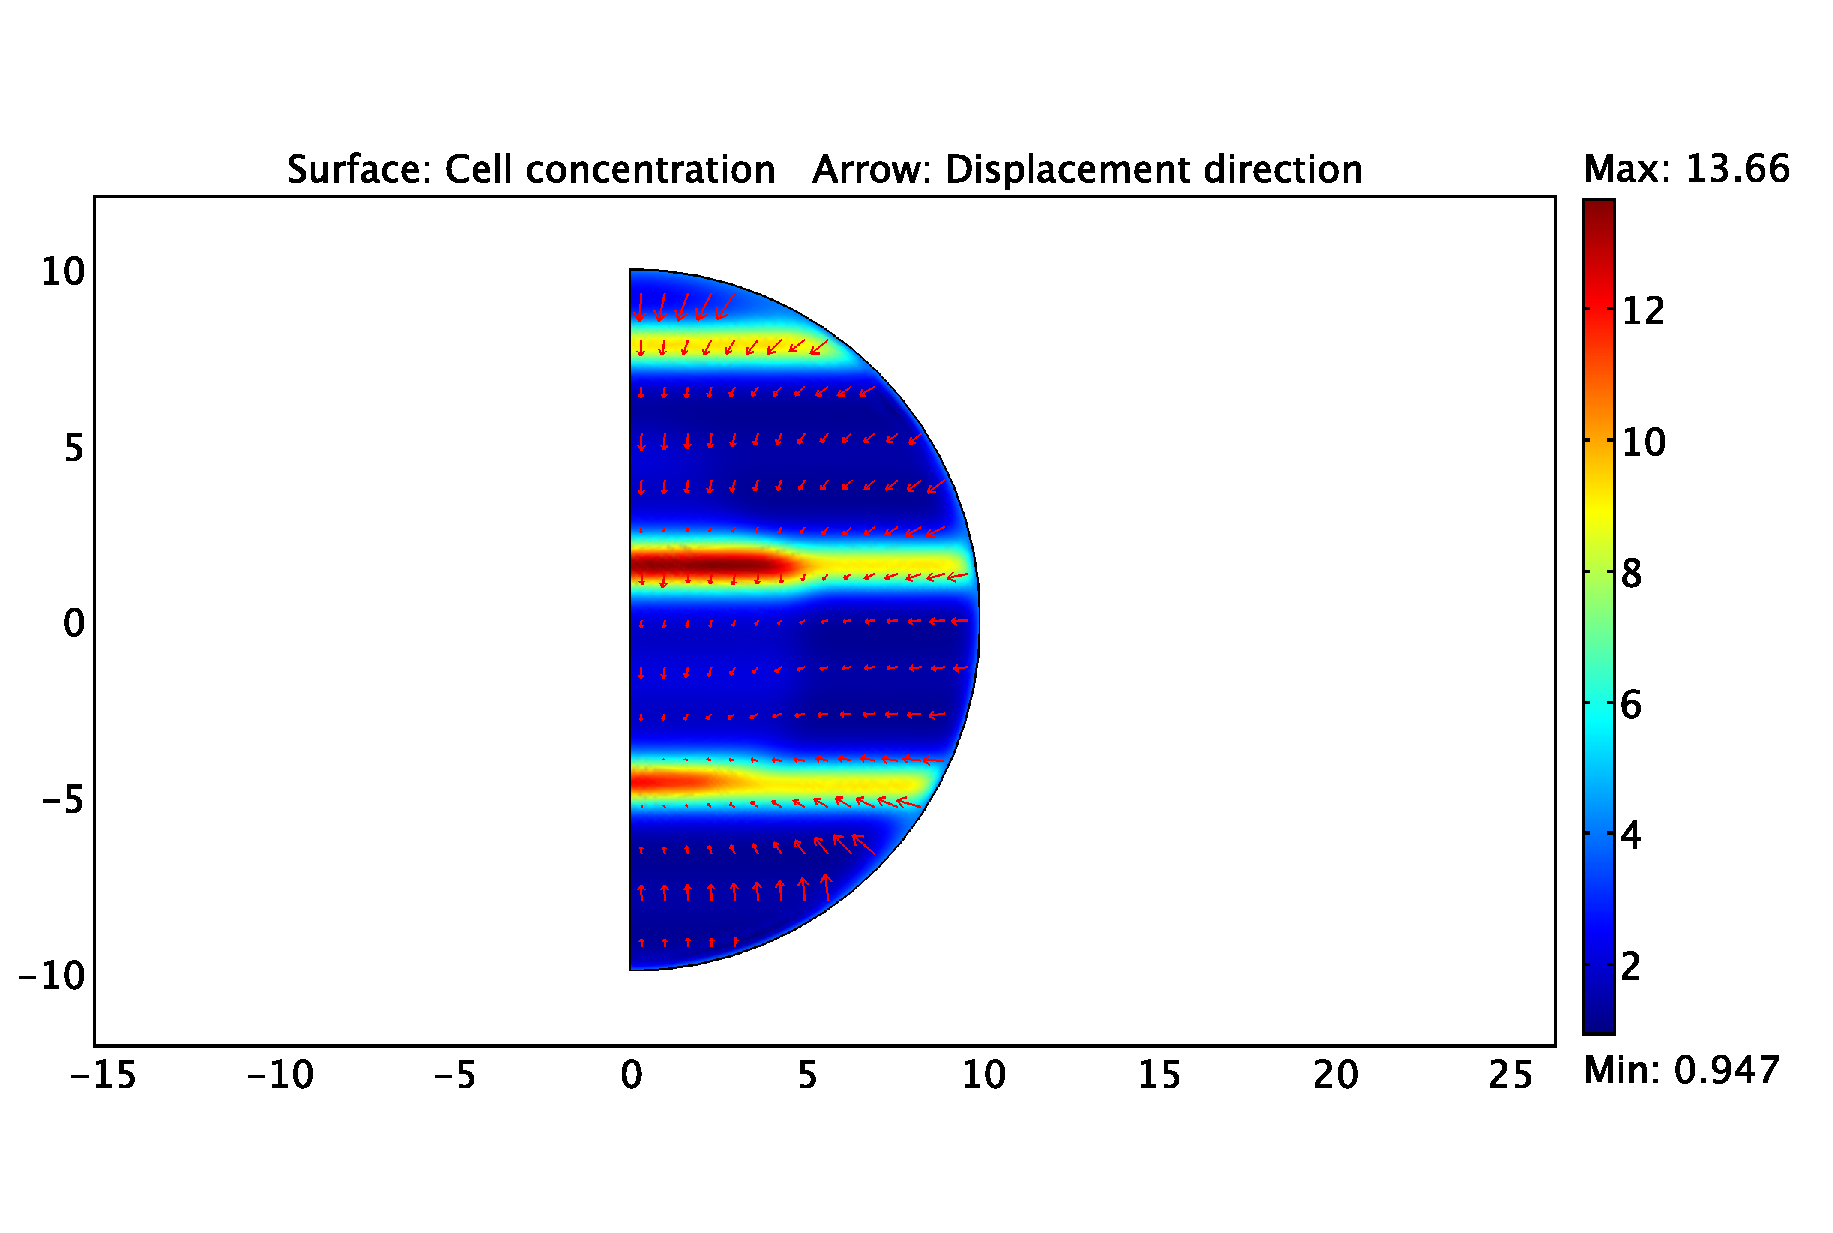
\includegraphics[width=0.8\textwidth]{images/examples/%
eulerian/cancer/haptotaxis-proliferating-cells-10}
\caption{Proliferating cells undergoing diffusion and haptotaxis at time $t=10$ days.}
\label{tumour-haptotaxis-proliferation-10}
\end{figure}

\subsection{Combining everything}
\label{cacophonous-medley}

\begin{figure}[!hptb]
\centering
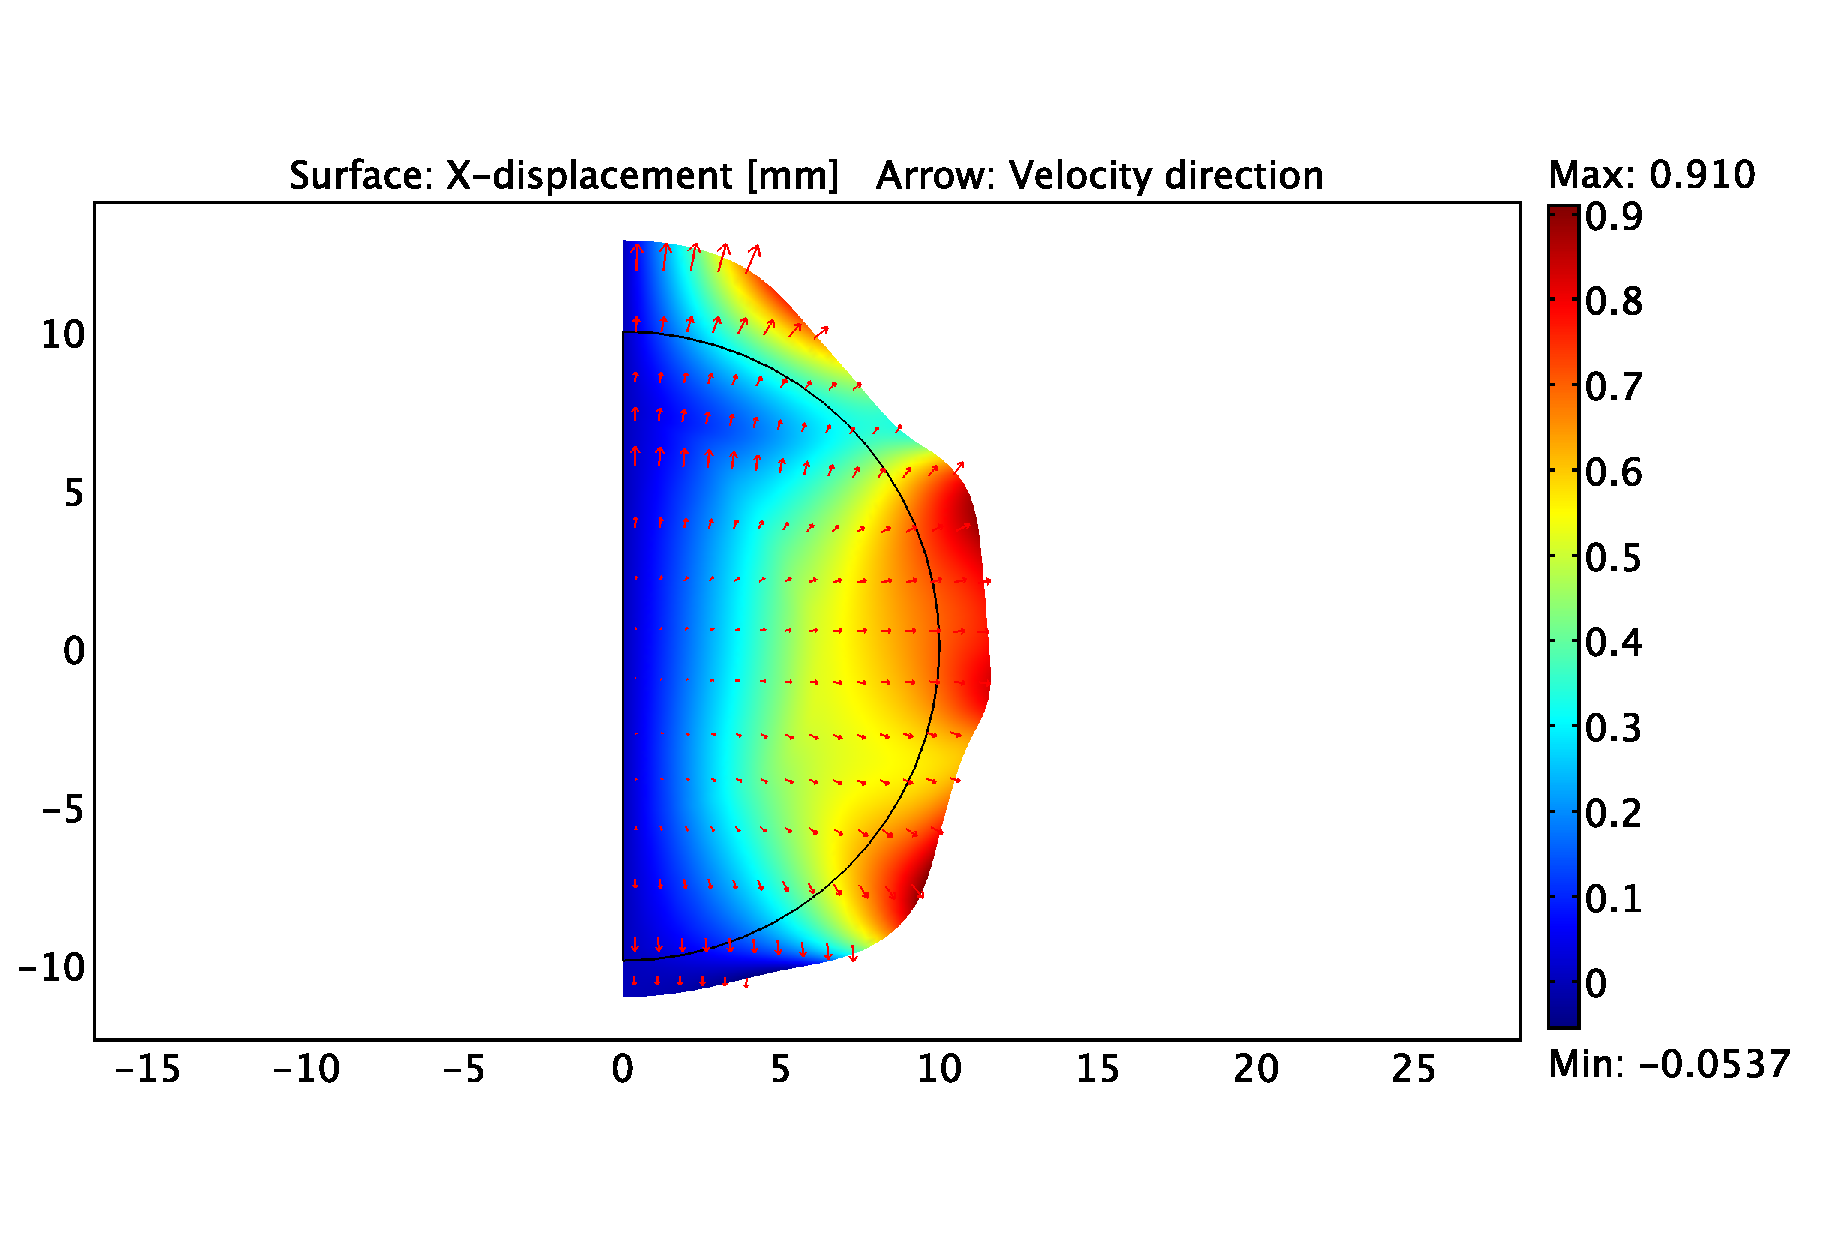
\includegraphics[width=0.8\textwidth]{images/examples/%
eulerian/cancer/growing-tumour-no-wall-4}
\caption{An unconstrained growing tumour at $t=4$ months.}
\label{tumour-growth-no-wall-4}
\end{figure}

\begin{figure}[!hptb]
\centering
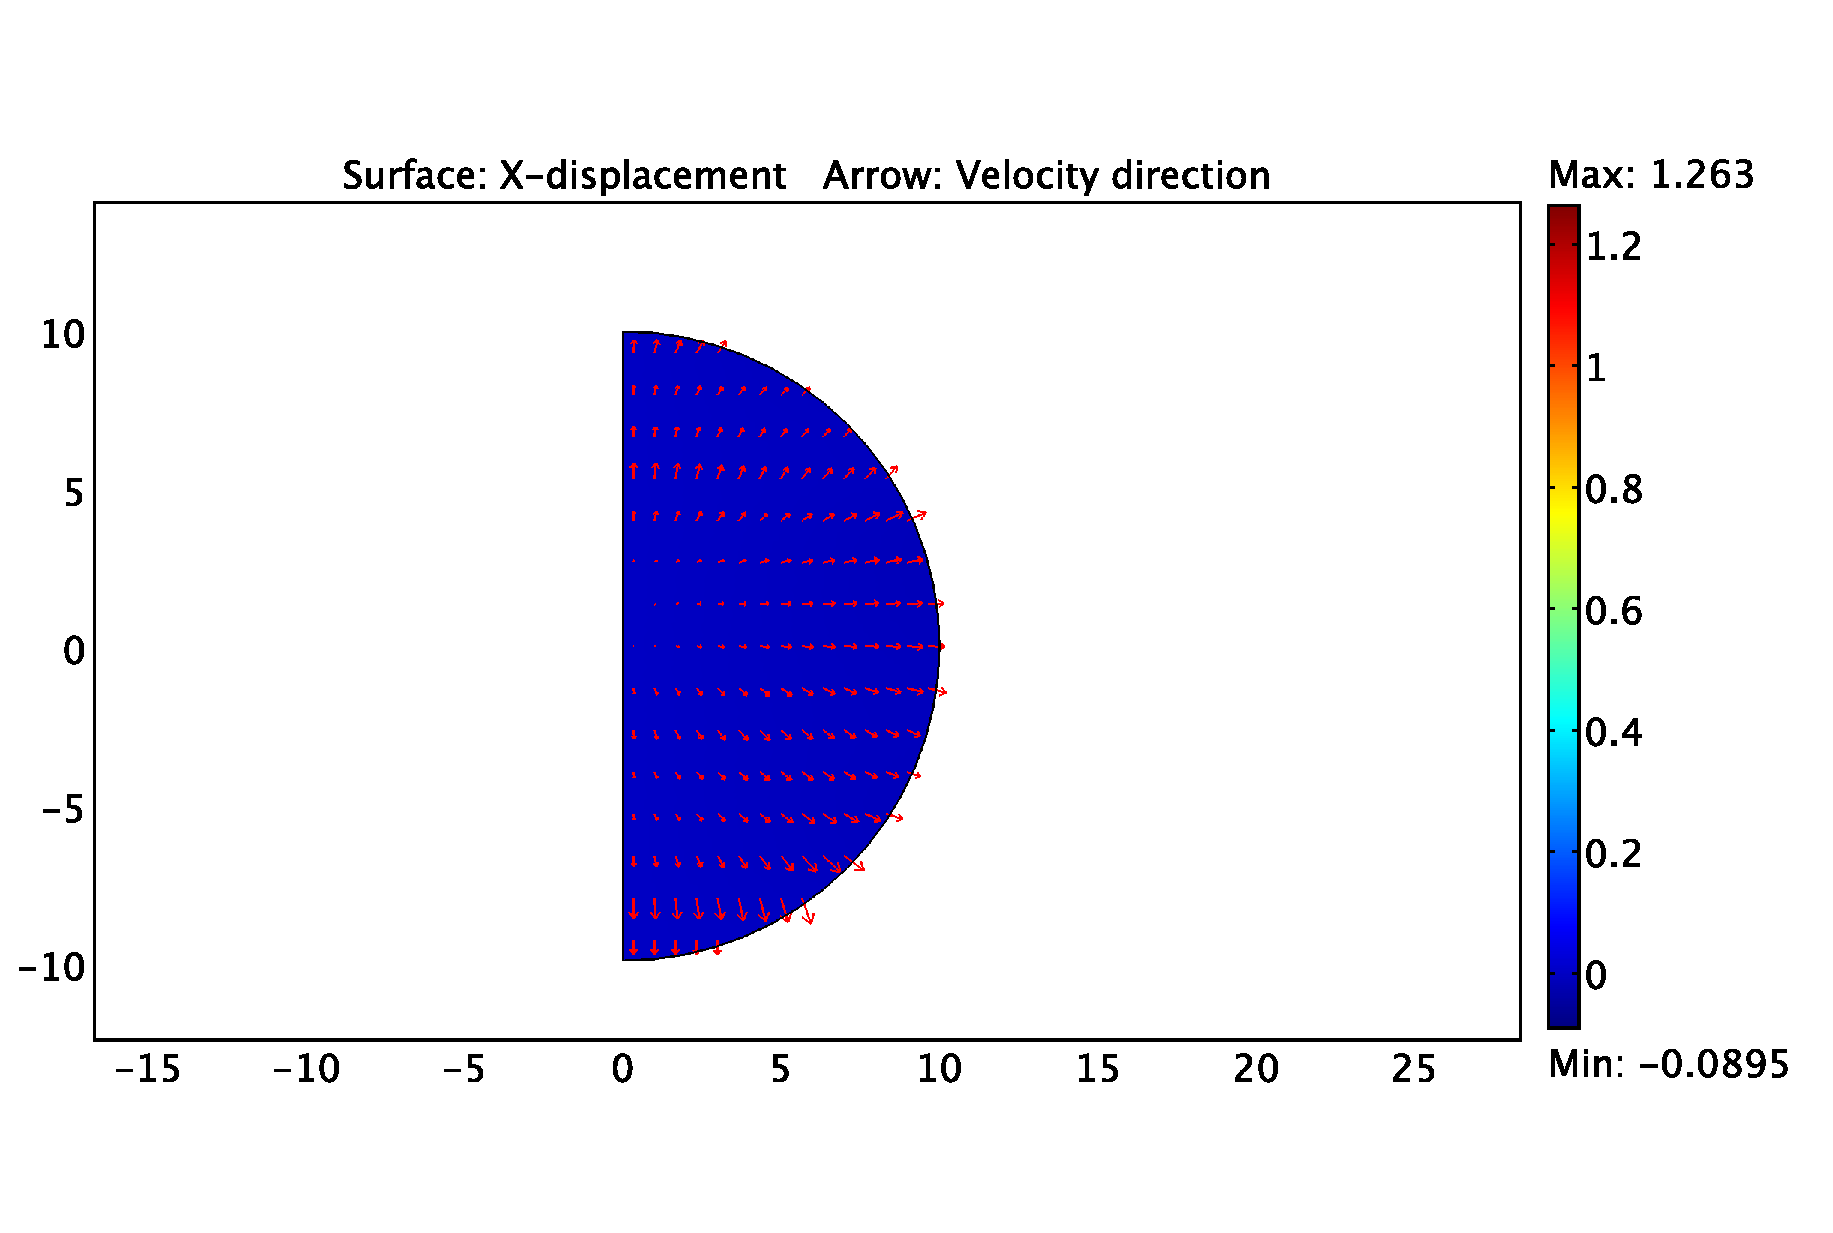
\includegraphics[width=0.8\textwidth]{images/examples/%
eulerian/cancer/growing-tumour-0.eps}
\caption{A constrained growing tumour at $t=0$ months.}
\label{tumour-growth-constrained-0}
\end{figure}

\begin{figure}[!hptb]
\centering
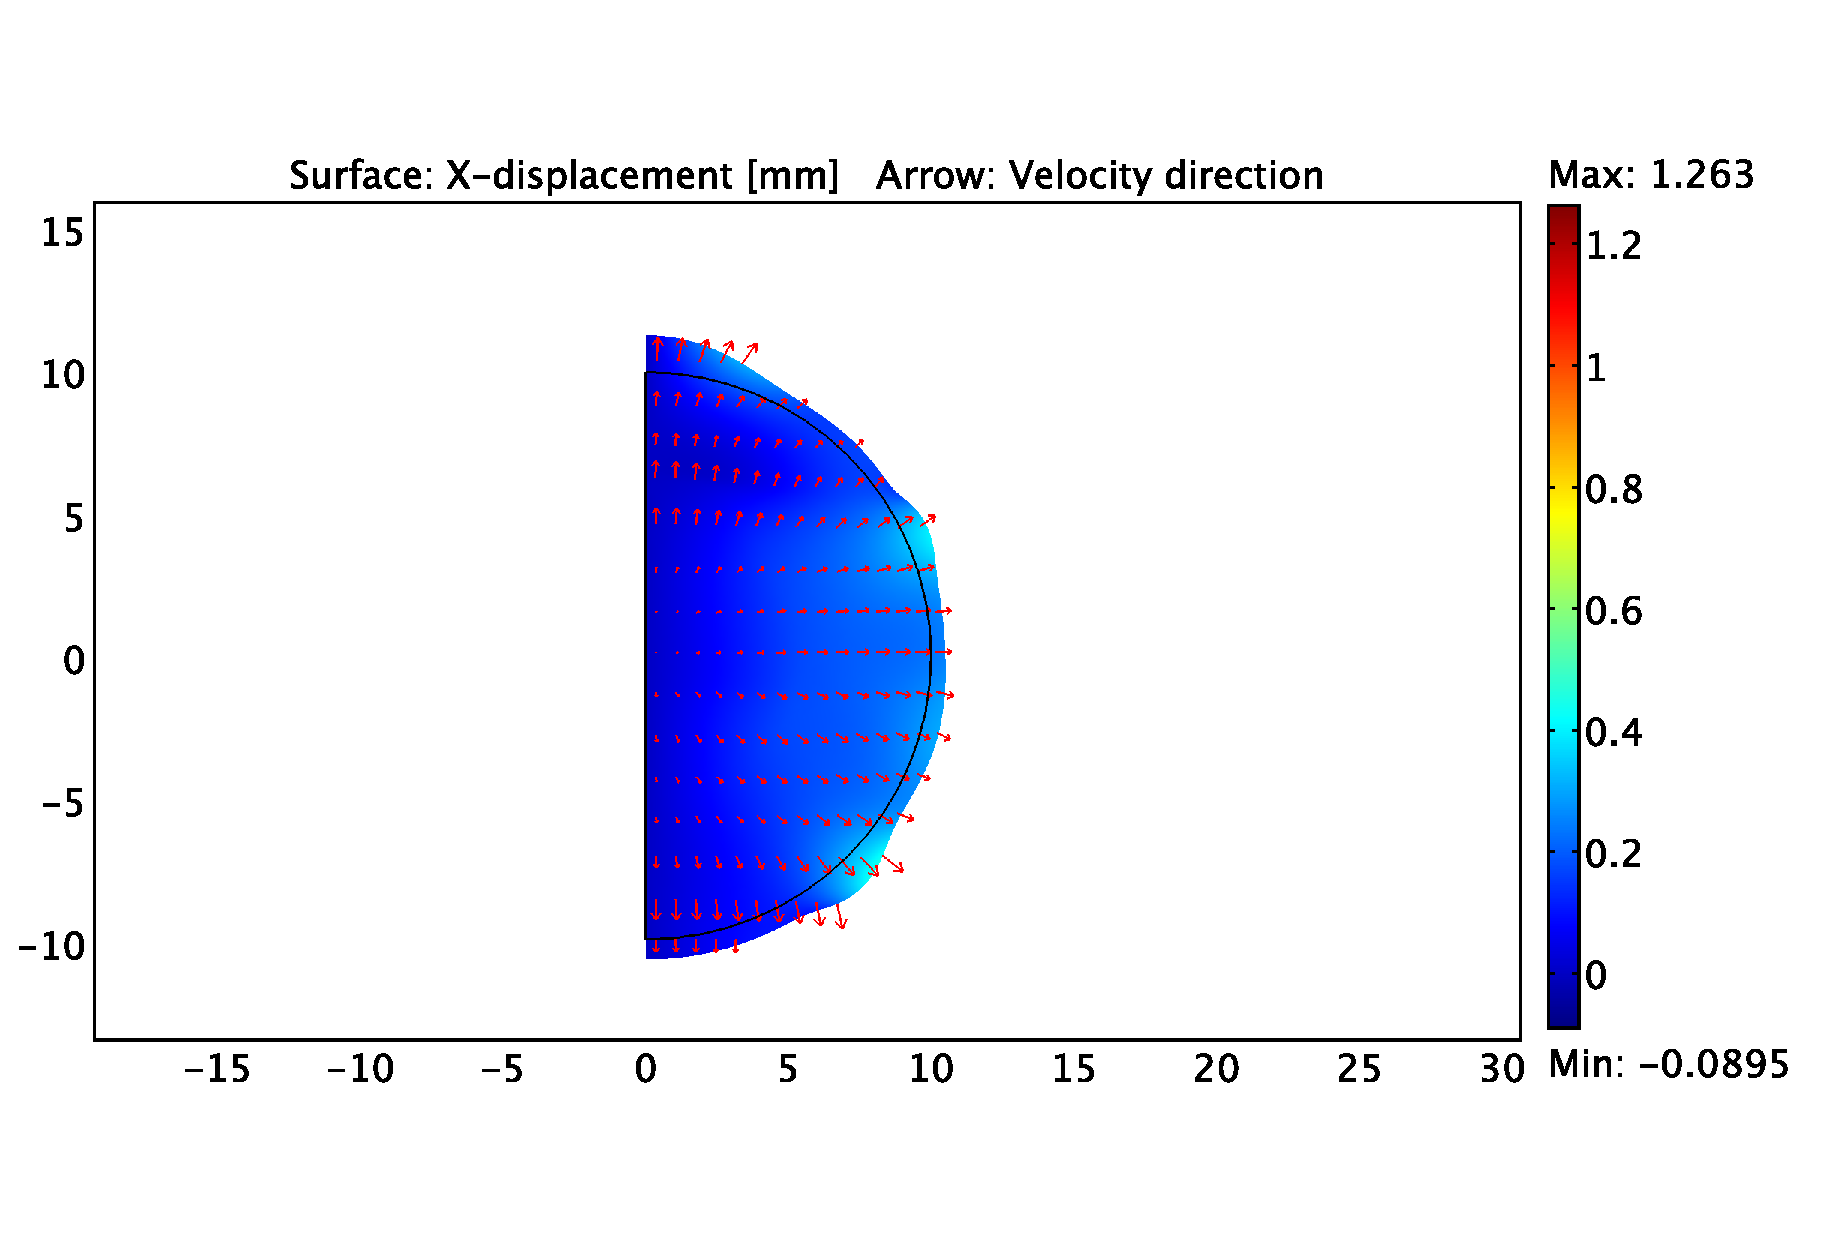
\includegraphics[width=0.8\textwidth]{images/examples/%
eulerian/cancer/growing-tumour-1.eps}
\caption{A constrained growing tumour at $t=1$ months.}
\label{tumour-growth-constrained-1}
\end{figure}

\begin{figure}[!hptb]
\centering
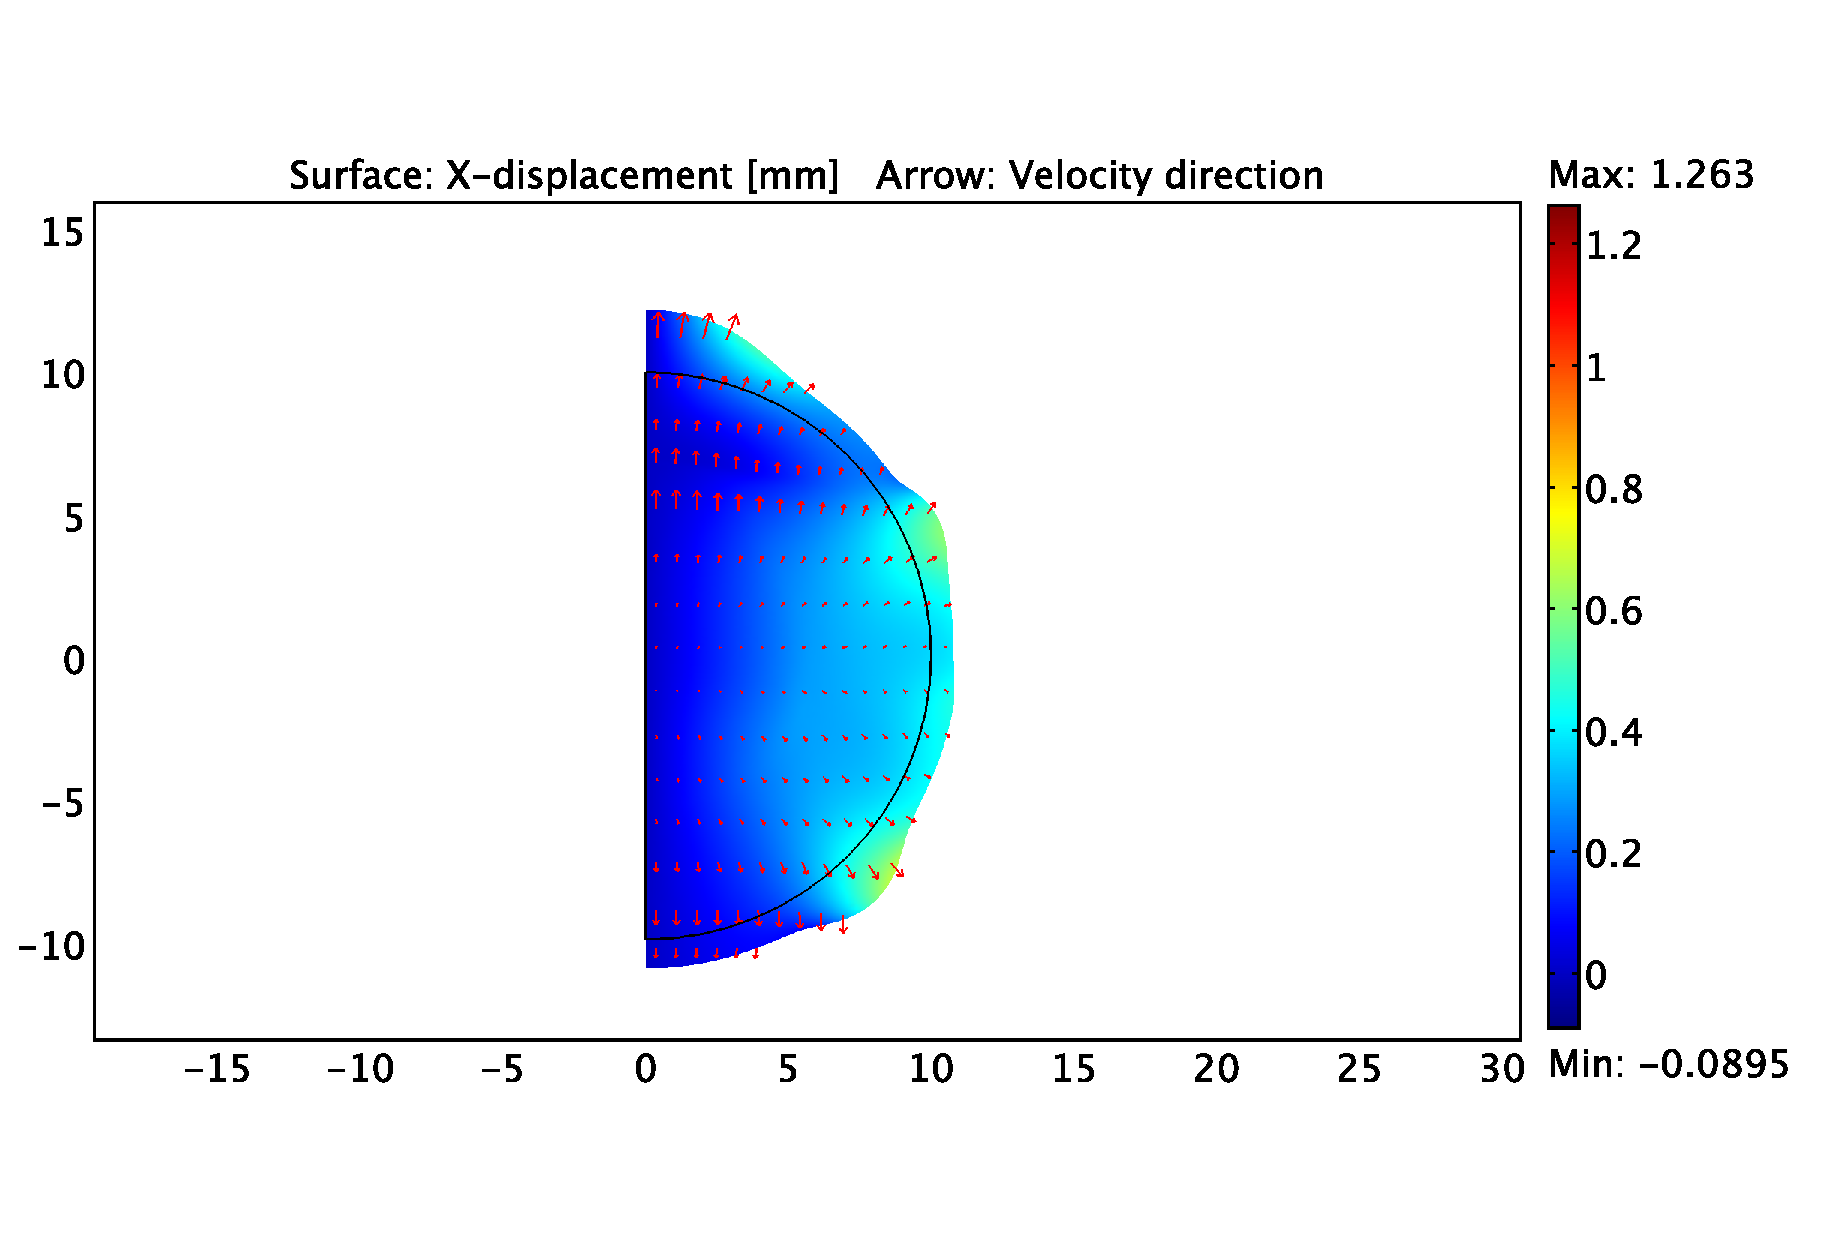
\includegraphics[width=0.8\textwidth]{images/examples/%
eulerian/cancer/growing-tumour-2.eps}
\caption{A constrained growing tumour at $t=2$ months.}
\label{tumour-growth-constrained-2}
\end{figure}

\begin{figure}[!hptb]
\centering
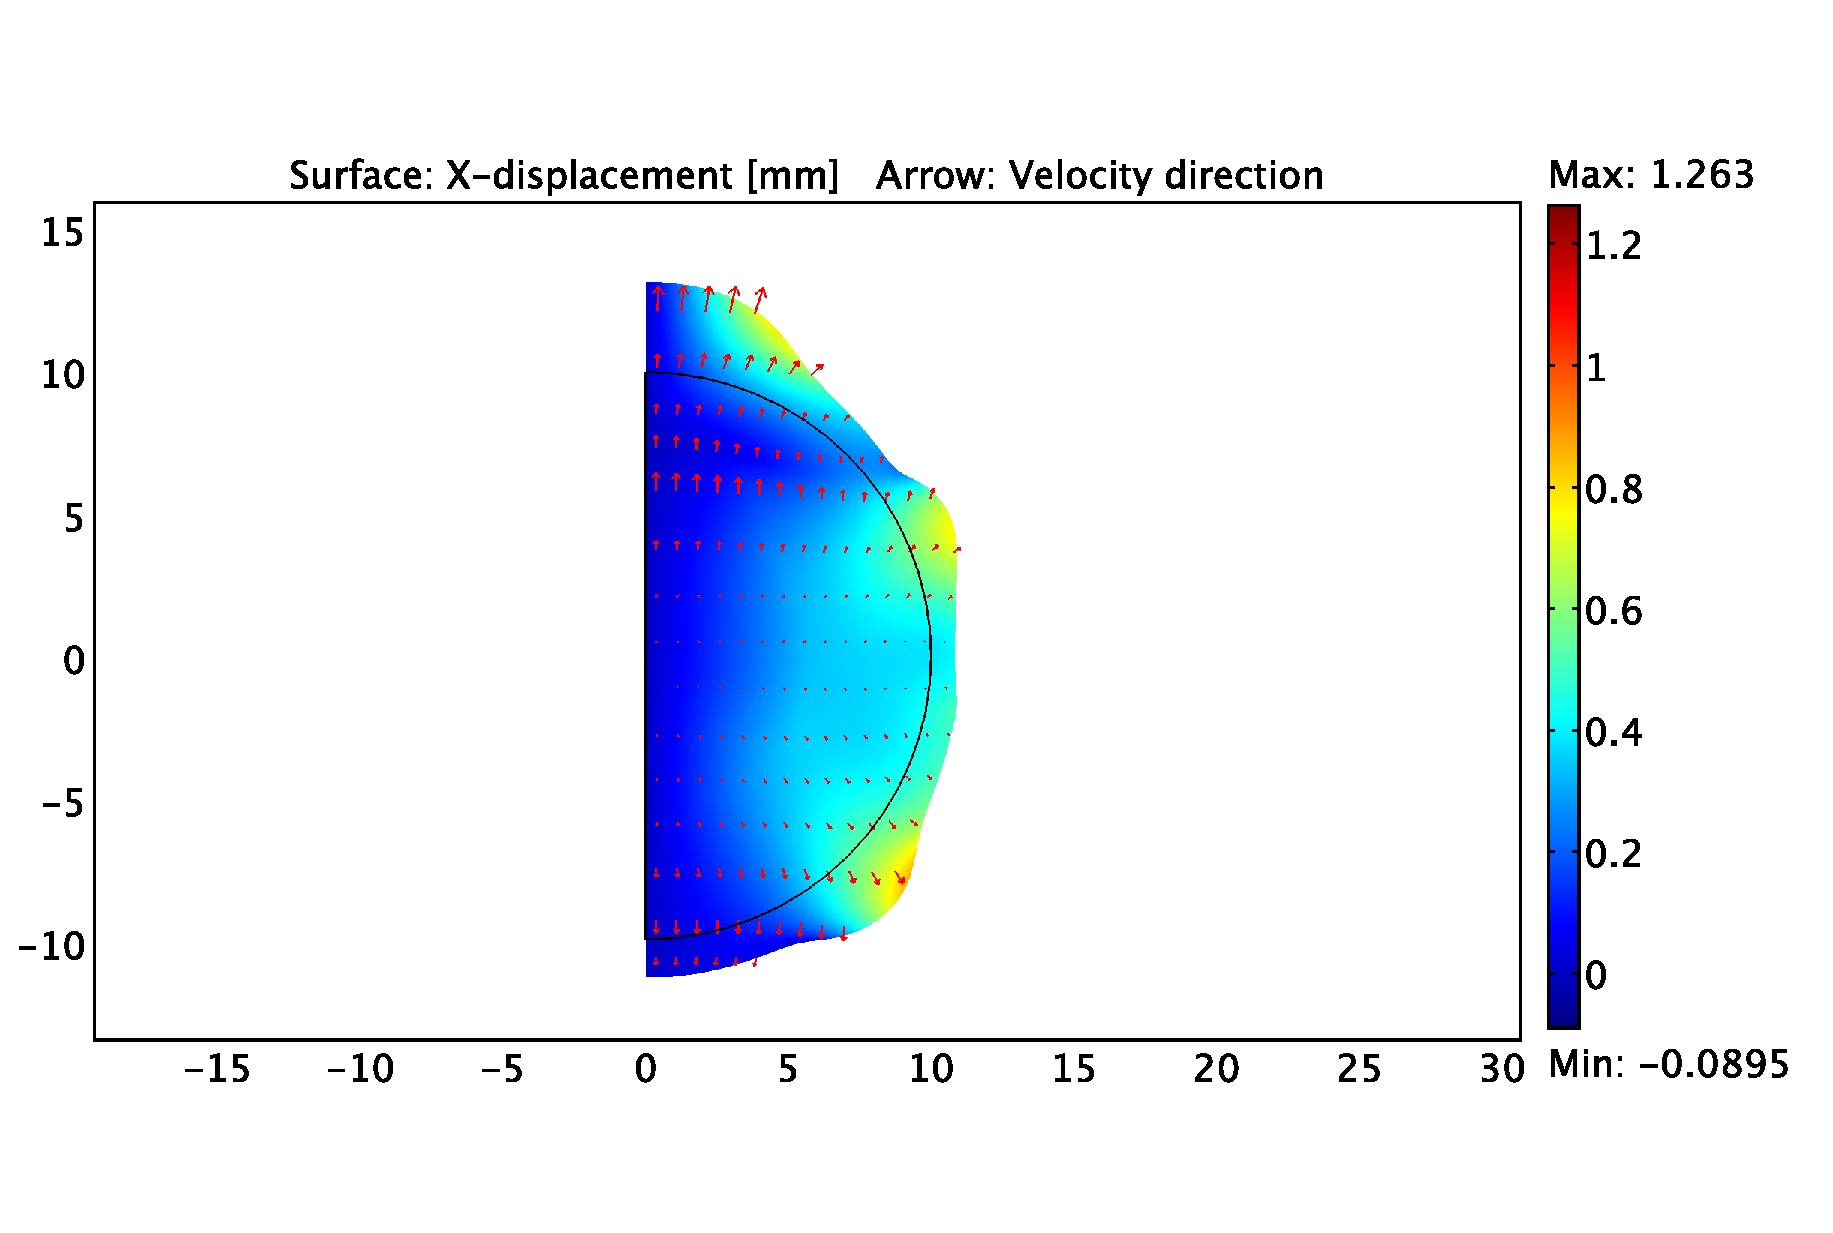
\includegraphics[width=0.8\textwidth]{images/examples/%
eulerian/cancer/growing-tumour-3.eps}
\caption{A constrained growing tumour at $t=3$ months.}
\label{tumour-growth-constrained-3}
\end{figure}

\begin{figure}[!hptb]
\centering
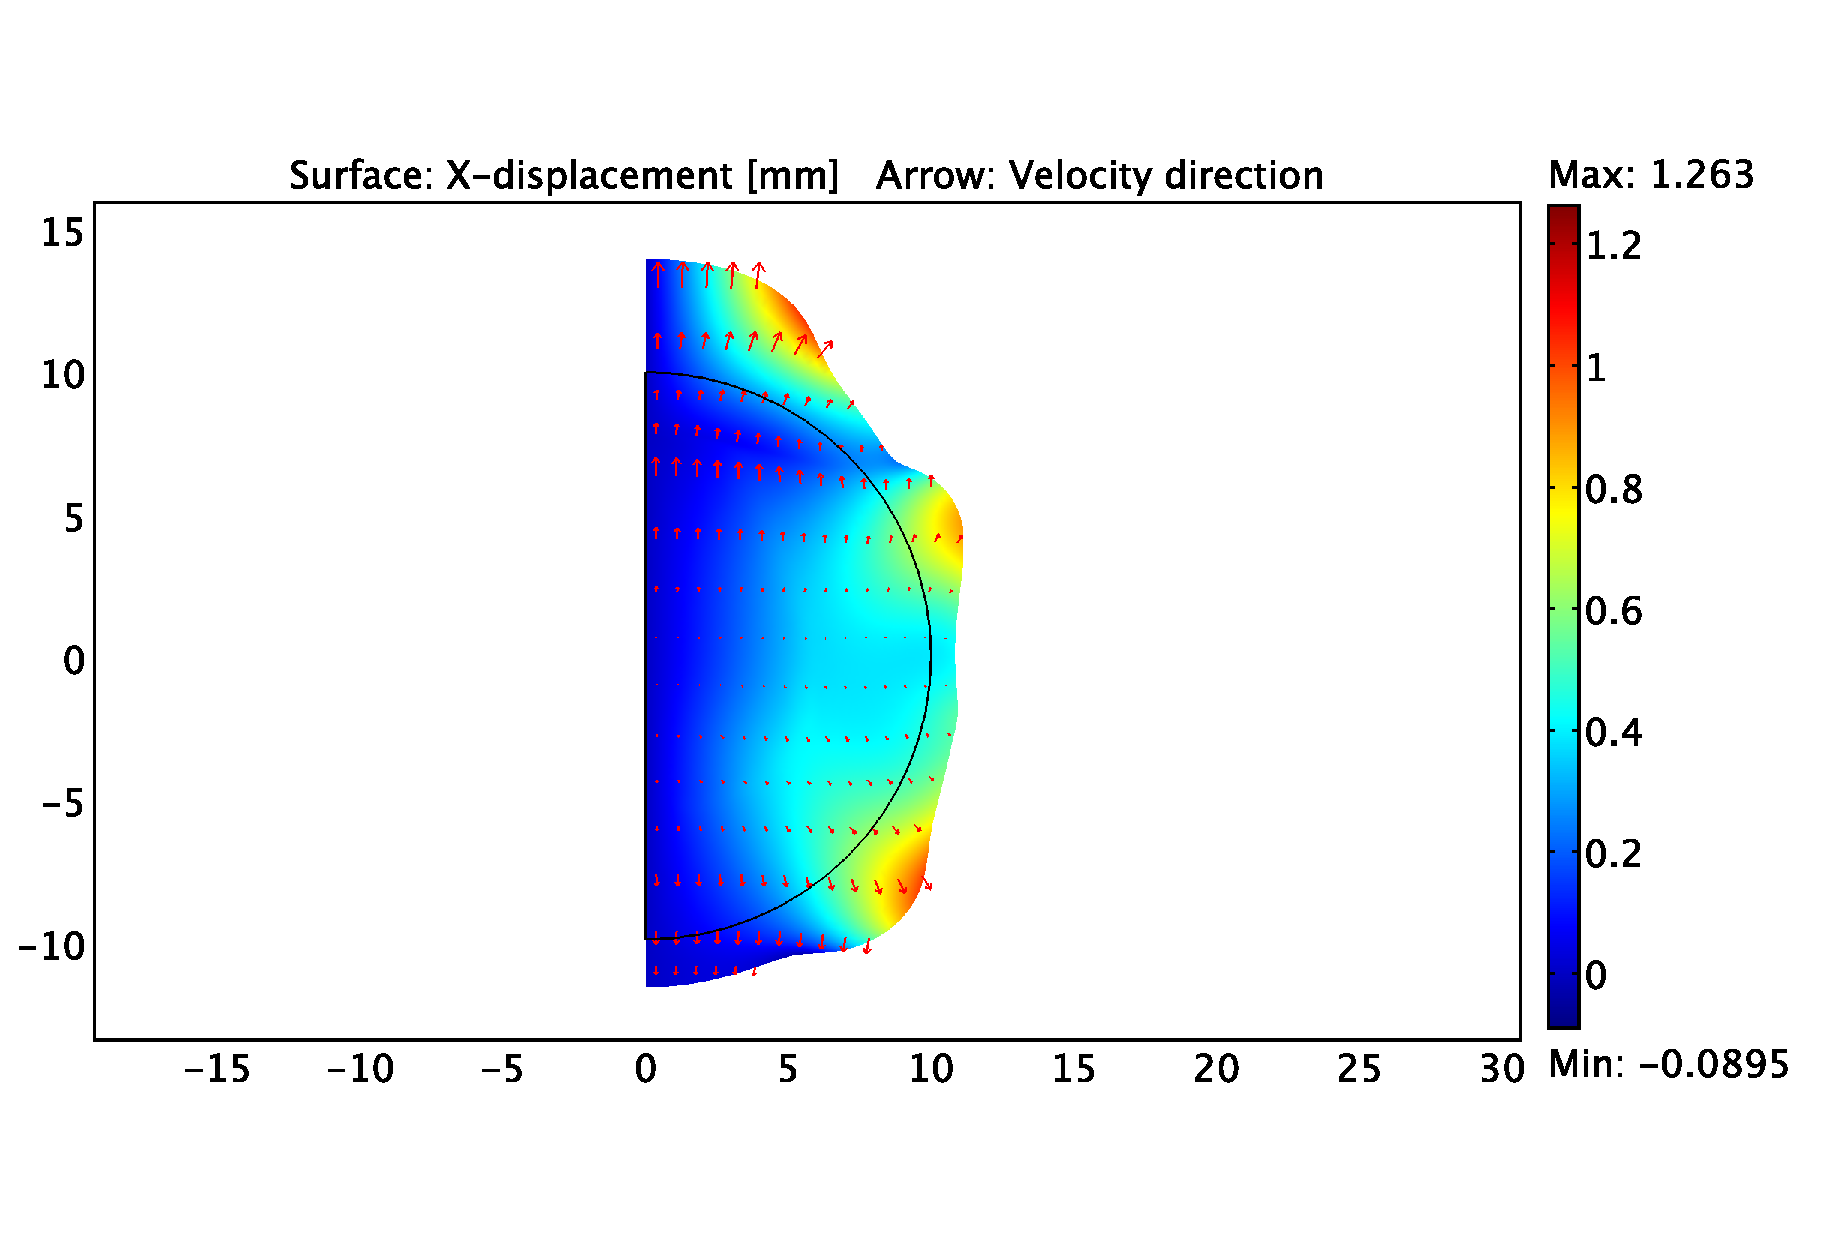
\includegraphics[width=0.8\textwidth]{images/examples/%
eulerian/cancer/growing-tumour-4.eps}
\caption{A constrained growing tumour at $t=4$ months.}
\label{tumour-growth-constrained-4}
\end{figure}

\begin{figure}[!hptb]
\centering
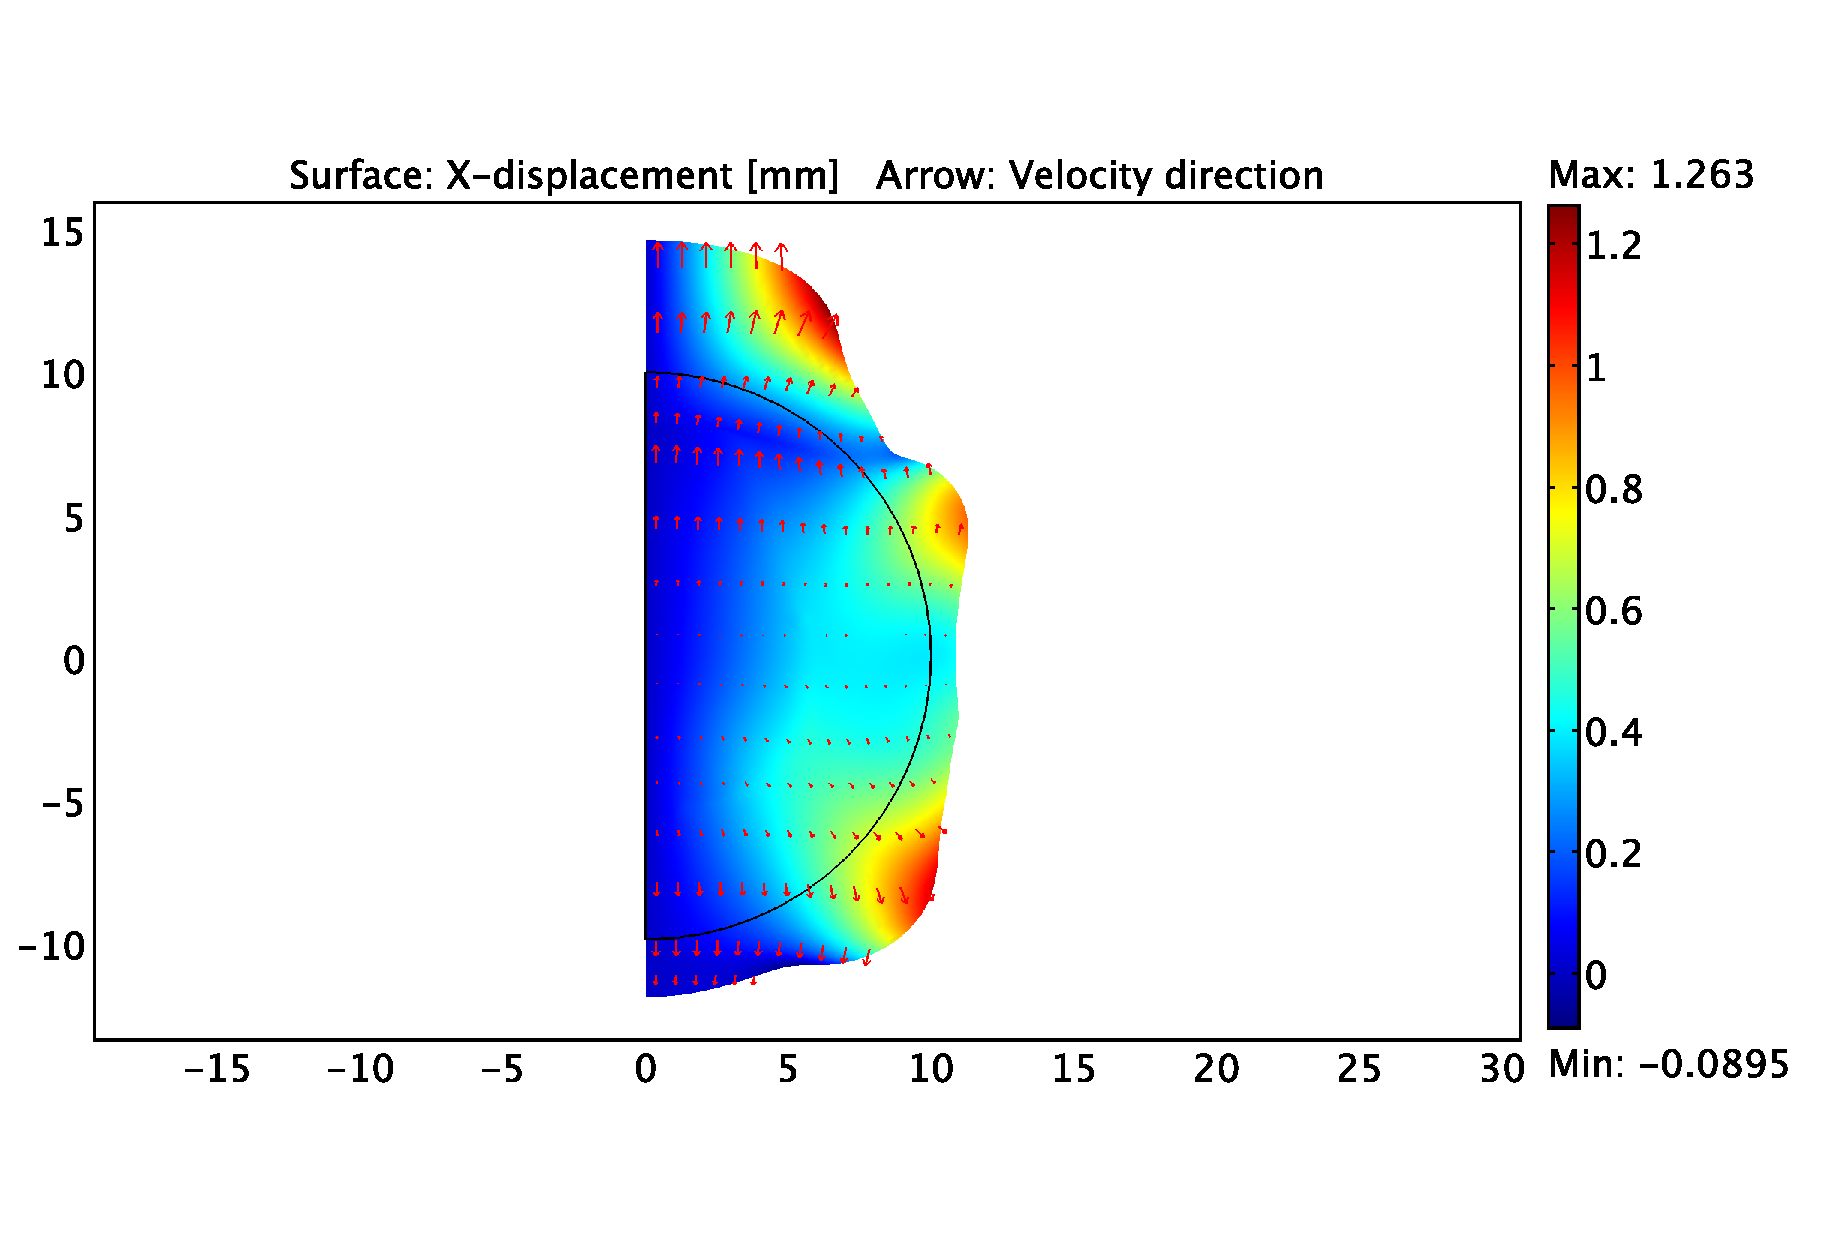
\includegraphics[width=0.8\textwidth]{images/examples/%
eulerian/cancer/growing-tumour-5.eps}
\caption{A constrained growing tumour at $t=5$ months.}
\label{tumour-growth-constrained-5}
\end{figure}


%

% Local Variables:
% TeX-master: "thesis"
% mode: latex
% mode: flyspell
% End:
